% !TEX encoding = UTF-8
\documentclass[a4paper,oneside,titlepage]{book}
\usepackage[italian]{babel}

\usepackage{amsmath}
\usepackage{amssymb}
\usepackage{enumitem}
\usepackage[nouppercase]{frontespizio}
\usepackage{galois}
\usepackage{graphicx}
\graphicspath{{./immagini/}}
\usepackage{hyperref}
\hypersetup{
    colorlinks=true,
    linkcolor=blue
}
\usepackage{multirow}
\usepackage{stmaryrd} % doppie parentesi quadre e simboli squadrati
\usepackage{subcaption}
\usepackage{xcolor}

% Tabelle:
\usepackage{array}
\usepackage{booktabs}
\usepackage{adjustbox}
\usepackage{makecell}

% Comandi:
%\newcommand{\rulesep}{\unskip\ \vrule\ }
\newcommand{\mail}[1]{\href{mailto:#1}{\texttt{#1}}}


\begin{document}
	
\begin{frontespizio}
	\Universita {Verona}
	\Dipartimento {Informatica}
	\Scuola {CdLM in Ingegneria e scienze informatiche}
	\Titolo {Fondamenti di analisi e verifica del software}
	\Sottotitolo {Riassunto del corso}
	\NCandidato {Creato da}
	\Candidato {Davide Zampieri}
	\Annoaccademico {2020-2021}
\end{frontespizio}

\frontmatter
{
  \hypersetup{linkcolor=black}
  \tableofcontents
}

\mainmatter
\chapter{Introduzione}

\section{Soddisfazione delle proprietà} % sezione 1 - slide 30/31,33,35,21,19
Le \textit{strategie} per la stima della soddisfazione di una certa proprietà sono:
\begin{itemize}
    \item \textit{Completeness} (inaccuratezza ottimistica), in cui si accettano anche alcuni programmi che non possiedono la proprietà (come nel caso del \textit{testing}).
    \item \textit{Soundness} (inaccuratezza pessimistica), in cui si suppone che il sistema non rispetti le specifiche (come nel caso dell'\textit{analisi statica} dove se non si riesce a dare una risposta allora si suppone che non valga la proprietà).
    \item \textit{Proprietà semplificate}, in cui si semplifica una proprietà troppo difficile (non verificabile) in una proprietà più semplice che può essere verificata (il problema sta nel fatto che non verifico la proprietà originale).
\end{itemize}
\begin{figure}[htp]
	\begin{subfigure}{0.49\textwidth}
	    \centering
		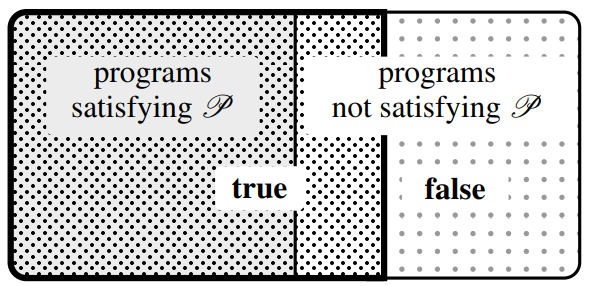
\includegraphics[width=\textwidth, height=\textheight, keepaspectratio]{completeness.png}
		\caption{Completeness}
	\end{subfigure}
	\hfill
	\begin{subfigure}{0.49\textwidth}
	    \centering
		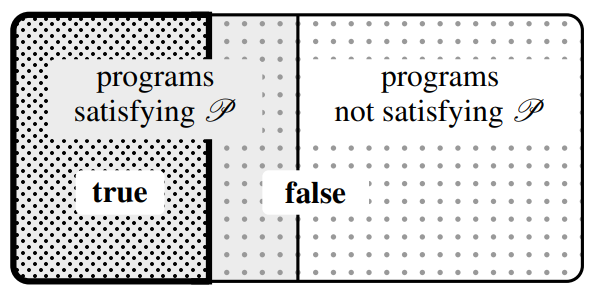
\includegraphics[width=\textwidth, height=\textheight, keepaspectratio]{soundness.png}
		\caption{Soundness}
	\end{subfigure}
\end{figure}


\section{Esempi} % sezione 1 - slide 36/37,46/47
\subsection{Buffer overflow}
Consiste nel far straripare un buffer, dal momento che in C non c'è il controllo sulle dimensioni degli array. Siccome nello stack si scrive verso il basso, se si arriva a sovrascrivere il \textit{return pointer} si può aprire una shell per poi andare ad eseguire codice malevolo.

\subsection{Pointer analysis}
Consiste nel guardare quando i puntatori sono legati alla stessa locazione di memoria. Questo in \textit{Java} può essere difficile dal momento che ogni variabile è considerata come un puntatore nascosto.

\begin{figure}[htp]
	\begin{subfigure}{0.49\textwidth}
	    \centering
		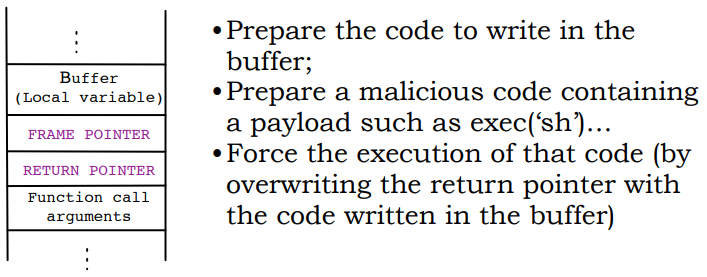
\includegraphics[width=\textwidth, height=\textheight, keepaspectratio]{buffer_overflow.png}
		\caption{Buffer overflow}
	\end{subfigure}
	\hfill
	\begin{subfigure}{0.49\textwidth}
	    \centering
		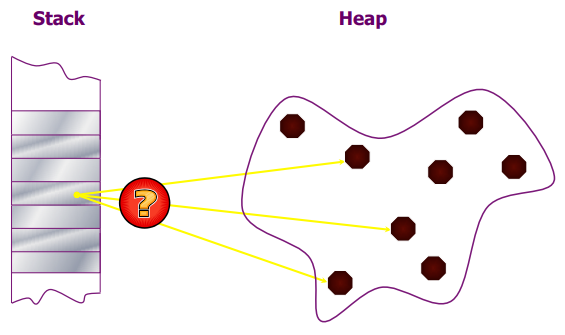
\includegraphics[width=\textwidth, height=\textheight, keepaspectratio]{java_pointers.png}
		\caption{Puntatori in Java}
	\end{subfigure}
\end{figure}


\section{Alcuni ingredienti} % sezione 1 - slide 49/50,51,53,60,62
\subsection{Astrazione matematica}
Consiste nello scartare i dettagli e nel creare un'interfaccia per manipolare meglio gli oggetti. Si possono quindi creare degli \textit{oggetti astratti} (ad es. grafi, matrici o relazioni) per cercare poi le \textit{soluzioni} di tali oggetti. Le proprietà verificate nell'astrazione dovranno valere anche nel codice. Ovviamente nel creare il modello matematico e nel definire le proprietà astratte perderò dei dettagli.
\begin{figure}[htp]
	\centering
	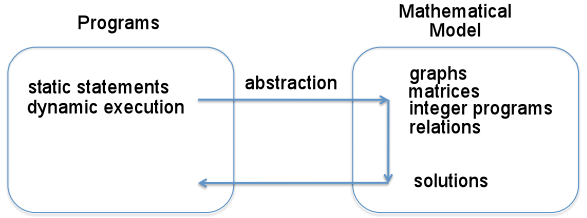
\includegraphics[width=\textwidth, height=\textheight, keepaspectratio]{absMat.png}
\end{figure}

\subsection{Semantica (vista come astrazione)}
\begin{itemize}
    \item \textit{Semantica operazionale}, in cui si descrivono le operazioni come sequenza di sotto-operazioni (operazioni diverse possono confluire nello stesso output).
    \item \textit{Semantica denotazionale}, in cui si associa con delle sequenze ogni input  al relativo output togliendo le sotto-operazioni (ad ogni input/output vengono associate tutte le tracce che hanno quell'input e quell'output).
\end{itemize}
\begin{figure}[htp]
	\begin{subfigure}{0.49\textwidth}
	    \centering
		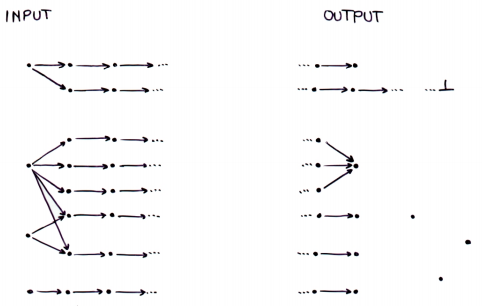
\includegraphics[width=\textwidth, height=\textheight, keepaspectratio]{semOp.png} 
		\caption{Semantica operazionale}
	\end{subfigure}
	\hfill
	\begin{subfigure}{0.49\textwidth}
	    \centering
		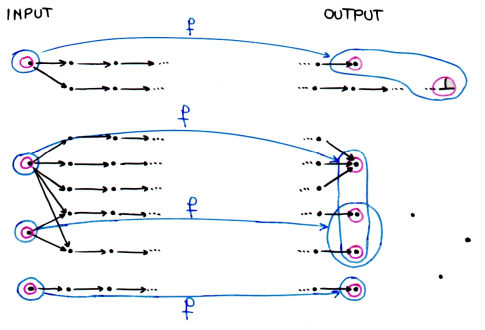
\includegraphics[width=\textwidth, height=\textheight, keepaspectratio]{semDen.png} 
		\caption{Semantica denotazionale}
	\end{subfigure}
\end{figure}

\subsection{Interpretazione astratta}
Quando, ad esempio, voglio verificare che in un programma si manipolino solo numeri interi, la proprietà che deve essere soddisfatta è quella dell'insieme delle parti. Nella \textit{figura (a)} sottostante viene mostrato come si può costruire un grafo che controlla che il programma abbia solo numeri interi: si può lavorare solo sui segni ma non si è in grado di valutare il dominio (non sembra essere quindi un'astrazione corretta).

\subsection{Control Flow Graph}
Rappresenta il \textit{flusso di controllo} di un programma, separando le informazioni di controllo dalla modifica della memoria. In sintesi, si divide il codice in base alle tipologie di operazioni che si fanno (ad es. branch o join).

\begin{figure}[htp]
	\begin{subfigure}{0.49\textwidth}
	    \centering
		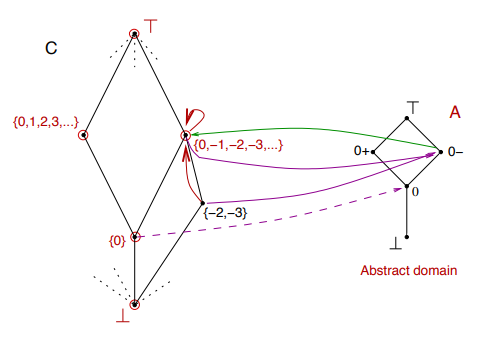
\includegraphics[width=\textwidth, height=\textheight, keepaspectratio]{absInt.png} 
		\caption{Interpretazione astratta}
	\end{subfigure}
	\hfill
	\begin{subfigure}{0.49\textwidth}
	    \centering
		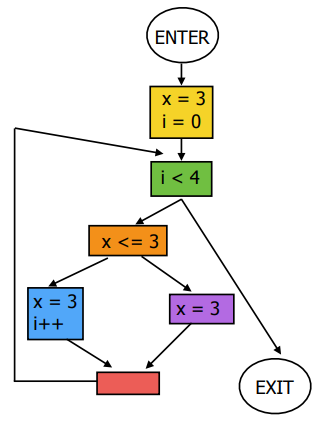
\includegraphics[width=\textwidth, height=\textheight, keepaspectratio]{cfg.png} 
		\caption{Control Flow Graph}
	\end{subfigure}
\end{figure}


\chapter{Modellare i programmi}

\section{Semantica delle tracce} % sezione 2a - slide 1-24
La \textit{semantica delle tracce}, o semantica delle esecuzioni, è l'insieme di tutte le possibili esecuzioni di un programma. Tali esecuzioni potrebbero essere infinite e generalmente sono deterministiche (per ogni istante di tempo si avrà un solo valore possibile). Inoltre, le tracce sono discretizzate ma è bene ricordare che sono anche potenzialmente infinite (i possibili stati iniziali per la sola variabile intera sono infatti infiniti). Infine, nella \textit{figura (b)} si può notare che la semantica delle tracce è formata da: stati iniziali, stati intermedi e stati finali (nel caso di tracce finite). In ogni caso, potrebbero esserci tracce infinite che non terminano.
\begin{figure}[htp]
	\begin{subfigure}{0.49\textwidth}
	    \centering
		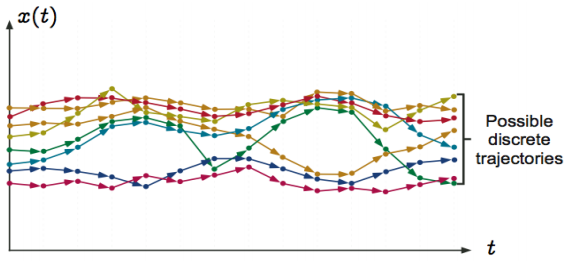
\includegraphics[width=\textwidth, height=\textheight, keepaspectratio]{semTracce1.png}
		\caption{Semantica delle tracce}
	\end{subfigure}
	\hfill
	\begin{subfigure}{0.49\textwidth}
	    \centering
		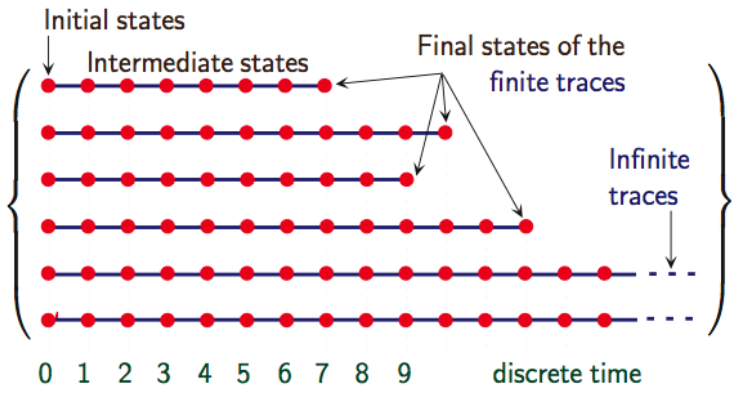
\includegraphics[width=\textwidth, height=\textheight, keepaspectratio]{semTracce2.png}
		\caption{Tipi di stato}
	\end{subfigure}
\end{figure}


\section{Semantica del punto fisso}
La \textit{semantica del punto fisso} è specificata da una coppia $<D,f>$ dove:
\begin{itemize}
    \item $D$ è il \textit{dominio semantico}, ovvero quello che ci interessa osservare della macchina.
    \item $f$ è la \textit{funzione di mapping}, ovvero una funzione totale, monotona (per preservare l'ordine) e iterabile (per poterla applicare a sé stessa continuamente) anche detta trasformatore semantico.
\end{itemize}

\subsection{Sistema di transizione}
La semantica operazionale di un linguaggio di programmazione associa ad ogni programma (scritto in quel linguaggio) un \textit{sistema di transizione}, ovvero una coppia $<\Sigma,\tau>$ dove:
\begin{itemize}
    \item $\Sigma$ è un insieme non vuoto di stati.
    \item $\tau \subseteq \Sigma \times \Sigma$ è la regola di transizione che permette di capire come passare allo stato successivo.
\end{itemize}


\section{Come costruire il punto fisso}
Se le tracce sono \textit{finite}, parto dal calcolo di tutte le possibili tracce che terminano:
\begin{itemize}
    \item Al passo zero non ho ancora nessuna traccia.
    \item Al primo passo prendo tutte le tracce di lunghezza 1 (stati terminali).
    \item Al secondo passo prendo gli stati terminali e tutti gli stati che terminano con un passo.
    \item Al terzo passo prenderò anche tutti gli stati che terminano con due passi, e così via.
\end{itemize}
Nelle figure sottostanti un pallino rosso rappresenta uno stato terminale, mentre un pallino blu rappresenta uno stato non terminale.
\begin{figure}[htp]
	\begin{subfigure}{0.49\textwidth}
	    \centering
		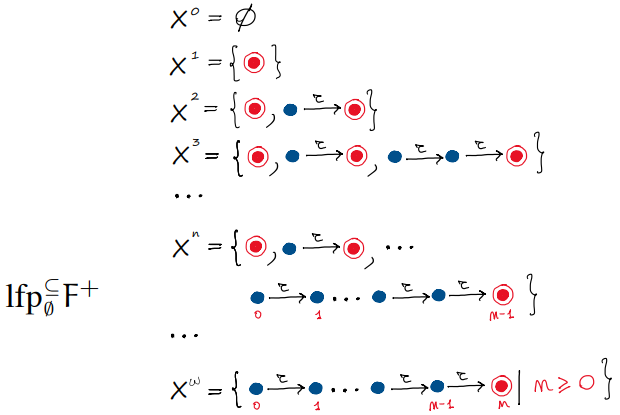
\includegraphics[width=0.8\textwidth]{fp1.png} 
		\caption{Per minimo punto fisso (lfp)}
	\end{subfigure}
	\hfill
	\begin{subfigure}{0.49\textwidth}
	    \centering
		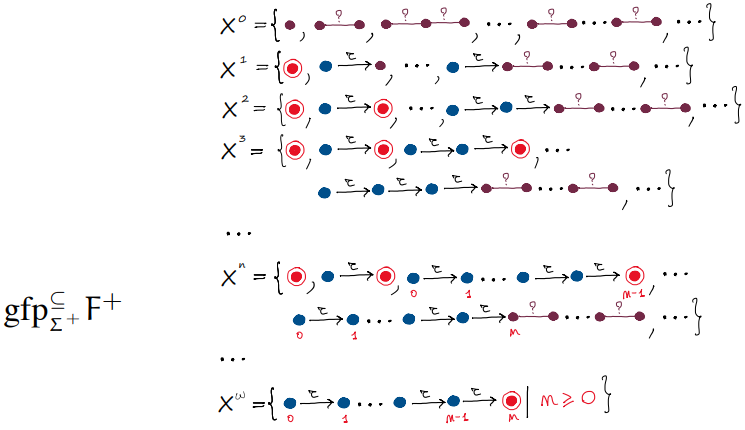
\includegraphics[width=0.9\textwidth]{fp2.png} 
		\caption{Per massimo punto fisso (gfp)}
	\end{subfigure}
\end{figure}

\noindent
Invece, se le tracce sono \textit{infinite}, si può costruire per minimo punto fisso scartando le tracce che ad ogni passo non rispettano la regola $\tau$:
\begin{figure}[htp]
	\centering
	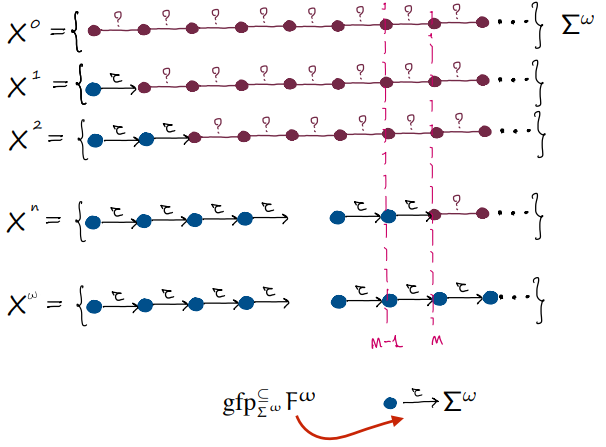
\includegraphics[width=0.4\textwidth]{fp3.png}
\end{figure}


\section{Control-Flow-Graph (CFG)} % sezione 2a - slide 25-40
Il \textit{Control Flow Graph} è generato dalla sintassi del programma e permette di capire la struttura del codice. Viene utilizzato per effettuare testing, debugging e per individuare codice morto. Un CFG è un \textit{grafo diretto} $G = <N,E>$ dove:
\begin{itemize}
	\item $n \in N$ sono i nodi che corrispondono ai punti di programma (basic blocks).
	\item $e = (n_i, n_j) \in E = N \times N$ sono gli archi, ovvero i passi di computazione (passaggi di controllo).
\end{itemize}

\subsection{Basic blocks}
I \textit{basic blocks} sono una sequenza massimale di comandi aventi un singolo entry point, un singolo exit point e nessun branch interno. Essi si costruiscono individuando i blocchi \textit{leader}:
\begin{itemize}
	\item Il primo statement del programma (entry point) è leader.
	\item Ogni statement che è target di un punto di branch è leader.
	\item Ogni statement che segue immediatamente un punto di branch è leader.
\end{itemize}
Quindi, un basic block è la sequenza di comandi che si trova tra un leader (incluso) e un altro leader (escluso).

\subsection{Generazione del CFG}
Dopo aver diviso il codice in basic blocks, essi verranno collegati dagli archi in corrispondenza di:
\begin{itemize}
	\item Salti (\textit{goto}) non condizionali.
	\item \textit{Branch condizionali} (che produrranno archi multipli).
	\item \textit{Flussi di programma} (quando non ci sono branch alla fine dei blocchi).
\end{itemize}
\begin{figure}[htp]
	\centering
	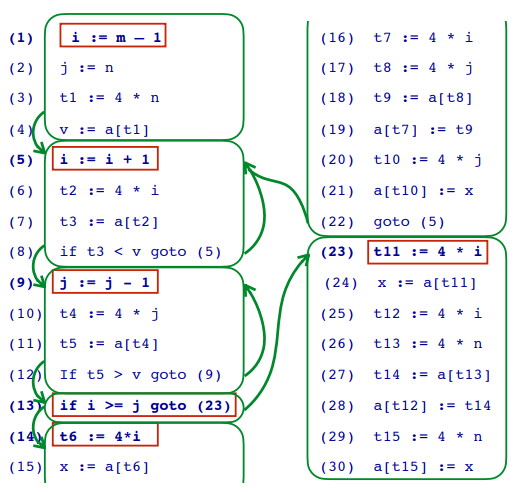
\includegraphics[width=0.5\textwidth]{cfgEx.png}
\end{figure}

\subsection{Notazione dei CFG}
Dato un CFG $G = <N,E>$ e un arco $(n_i, n_j) \in E$:
\begin{itemize}
	\item $n_i$ è detto \textit{predecessore} di $n_j$.
	\item $n_j$ è detto \textit{successore} di $n_i$.
\end{itemize}	
Inoltre, per ogni nodo $n\in N$:
\begin{itemize}
	\item $Pred(n)$ è l'insieme dei predecessori del nodo $n$.
	\item $Succ(n)$ è l'insieme dei successori del nodo $n$.
	\item \`{E} detto \textit{branch node} un nodo che ha più di un successore.
	\item \`{E} detto \textit{join node} un nodo che ha più di un predecessore.
\end{itemize}

\subsection{Linguaggio e semantica di IMP-CFG}
In questo linguaggio (leggermente diverso da IMP) gli \textit{archi} vengono etichettati con l'\textit{effetto del comando} e sono della forma $k = (u, lab, v)$ dove $u$ è il nodo sorgente, $v$ è il nodo di destinazione e $lab$ è l'etichetta. Una \textit{computazione} è quindi un percorso (insieme di archi del CFG) che va da un nodo di partenza $u$ a un nodo terminale $v$:
\[
    \pi = k_1 ... k_n, k_i = (u_i, lab_i, u_{i+1}), i = 1 ... n-1, u = u_1, v = u_n
\]
La \textit{trasformazione dello stato} è data invece dalla composizione degli effetti degli archi:
\[
	\llbracket \pi \rrbracket = \llbracket k_n \rrbracket \circ ... \circ \llbracket k_1 \rrbracket
\]
\begin{figure}[htp]
	\begin{subfigure}{0.49\textwidth}
	    \centering
		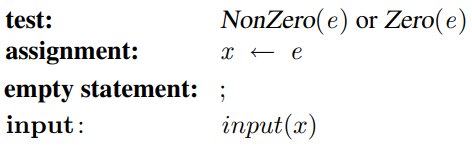
\includegraphics[width=\textwidth, height=\textheight, keepaspectratio]{impCfgLang.png}
		\caption{Linguaggio IMP-CFG}
	\end{subfigure}
	\hfill
	\begin{subfigure}{0.49\textwidth}
	    \centering
		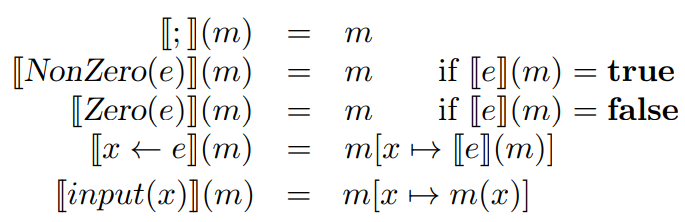
\includegraphics[width=\textwidth, height=\textheight, keepaspectratio]{impCfgSem.png} 
		\caption{Semantica di IMP-CFG}
	\end{subfigure}
\end{figure}


\chapter{Approssimare il significato dei programmi}

\section{Interpretazione astratta} % sezione 2b - slide 2-4
Data una proprietà $Q$, voglio renderla decidibile (ma ho una semantica concreta che non è decidibile). L'\textit{idea} di base è quella di trovare un'approssimazione $\llbracket P \rrbracket^{\#}$ della semantica $\llbracket P \rrbracket$ tale per cui valgano:
\begin{itemize}
	\item \textit{Correttezza}: $\llbracket P \rrbracket \subseteq \llbracket P \rrbracket^{\#}$.
	\item \textit{Decidibilità}: $\llbracket P \rrbracket^{\#} \subseteq Q$.
\end{itemize}
Se entrambe le proprietà sono soddisfatte (la semantica concreta deve essere contenuta in quella astratta la quale deve essere decidibile), allora vale che $\llbracket P \rrbracket^{\#} \subseteq Q \Rightarrow \llbracket P \rrbracket \subseteq Q$; altrimenti non so dire nulla. La \textit{semantica} sarà specificata da una coppia $<D,f>$ dove $D$ è un dominio semantico ordinato e $f$ è una funzione con una soluzione a punto fisso. Quello che dobbiamo studiare sarà quindi:
\begin{itemize}
    \item L'astrazione degli oggetti e la relazione tra rappresentazione astratta e concreta.
    \item L'astrazione del calcolo del punto fisso nel caso della rappresentazione astratta.
\end{itemize}


\section{Un esempio di oggetto: il fiore} % sezione 2b - slide 5-25
Un oggetto può essere rappresentato come una coppia formata da un'\textit{origine} e un \textit{insieme finito di pixel neri} (su sfondo bianco).
\begin{figure}[htp]
	\centering
	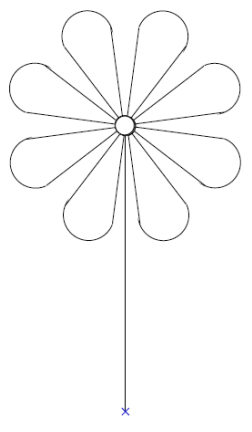
\includegraphics[width=0.1\textwidth]{fiore.png}
\end{figure}

\subsection{Operazioni}
\begin{itemize}
    \item \textit{Costante} $petal$: l'oggetto è formato solo dall'origine e dai pixel del petalo.
    \item \textit{Rotazione} $r[a](o)$: l'oggetto $o$ viene ruotato di $a$ gradi lasciando l'origine fissa.
    \item \textit{Unione} $o_1 \cup o_2$: giustappone gli oggetti unendo le origini.
    \item \textit{Funzione} $stem$: aggiunge uno stelo nell'origine e sposta l'origine alla radice.
\end{itemize}
\begin{figure}[htp]
	\begin{subfigure}{0.49\textwidth}
	    \centering
		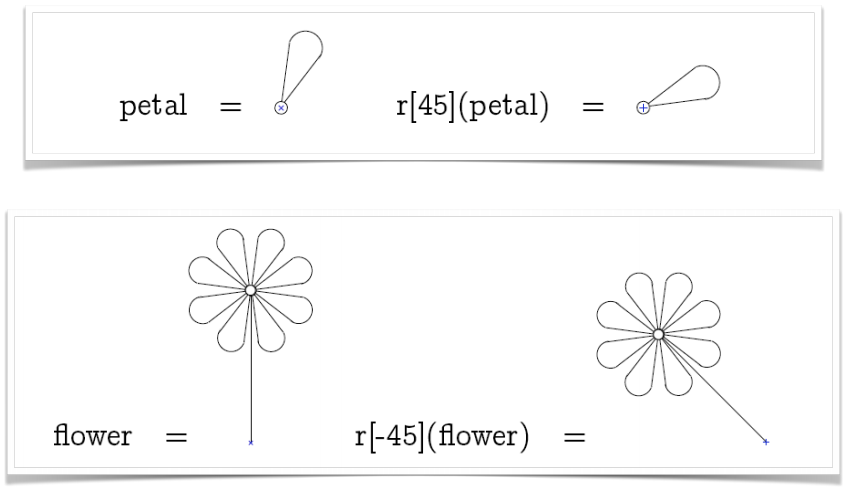
\includegraphics[width=0.8\textwidth]{fioriOp1.png}
		\caption{Petalo e rotazione}
	\end{subfigure}
	\hfill
	\begin{subfigure}{0.49\textwidth}
		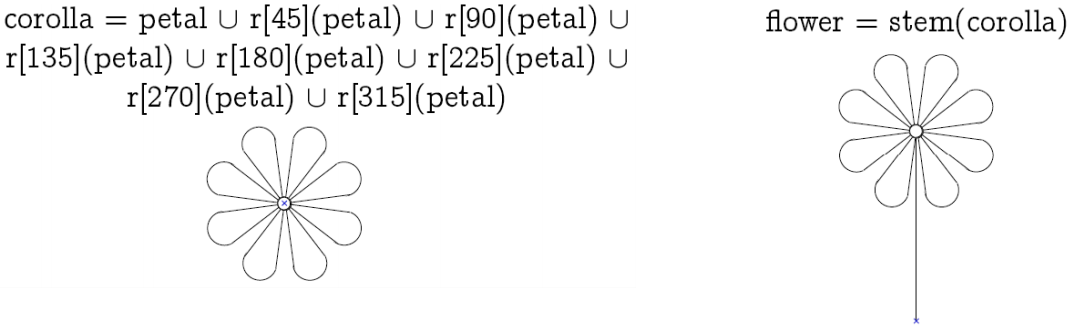
\includegraphics[width=\textwidth, height=\textheight, keepaspectratio]{fioriOp2.png}
		\caption{Unione e stelo}
	\end{subfigure}
\end{figure}

\subsection{Sovra-approssimazione}
La \textit{sovra-approssimazione} di un oggetto è un oggetto avente la stessa origine ma un insieme di pixel più ampio. Ad esempio, un fiore lo posso descrivere come un poligono (aggiungo del rumore). Possiamo però notare che c'è una \textit{relazione d'ordine} tra il fiore e il poligono, ovvero che il mondo astratto (poligono) ha meno dettagli ma contiene l'oggetto concreto (fiore).
\begin{figure}[htp]
	\begin{subfigure}{0.49\textwidth}
	    \centering
		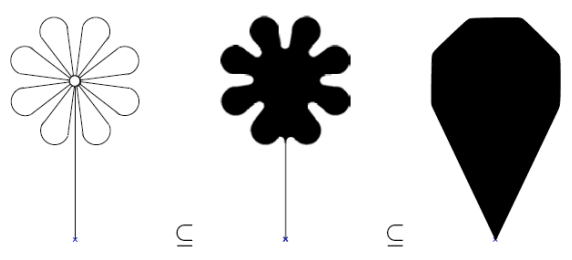
\includegraphics[width=0.7\textwidth]{uppApp1.png}
		\caption{Sovra-approssimazione di un fiore}
	\end{subfigure}
	\hfill
	\begin{subfigure}{0.49\textwidth}
	    \centering
		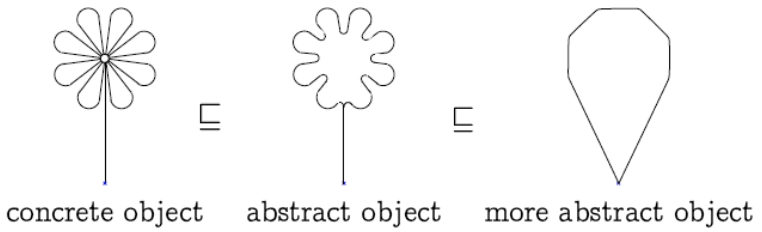
\includegraphics[width=\textwidth, height=\textheight, keepaspectratio]{uppApp2.png} 
		\caption{Relazione d'ordine tra fiore e poligono}
	\end{subfigure}
\end{figure}

\subsection{Oggetti e domini astratti}
Un \textit{oggetto astratto} è una rappresentazione matematica dell'approssimazione di un oggetto concreto (il concreto è contenuto nell'astratto). Un \textit{dominio astratto}, invece, è l'insieme degli oggetti astratti e delle funzioni astratte che rappresentano le operazioni concrete.

\subsection{Funzioni di astrazione e concretizzazione}
L'\textit{astrazione} avviene per mezzo di una funzione $\alpha$ che mappa ogni oggetto concreto $o$ nella sua rappresentazione astratta $\alpha(o)$. La \textit{concretizzazione}, invece, avviene per mezzo di una funzione $\gamma$ che mappa ogni oggetto astratto $\bar{o}$ nell'oggetto concreto $\gamma(\bar{o})$ che rappresenta.

\subsection{Connessioni di Galois}
Le funzioni $\alpha$ e $\gamma$ sono \textit{monotone}, ovvero se due oggetti concreti (o astratti) sono in relazione tra loro allora lo devono essere anche nella rispettiva rappresentazione astratta (o concreta). Ciò significa che se parto dal concreto, astraggo e poi ri-concretizzo devo ottenere qualcosa di più grande rispetto al concreto (fare $\gamma(\alpha(x))$ cambia il risultato rispetto all'inizio). Viceversa, nell'astrarre dopo una concretizzazione non perdo nulla perché avevo già scartato tutti i dettagli (fare $\alpha(\gamma(y))$ lascia invariato il risultato rispetto all'inizio).
\begin{figure}[htp]
	\begin{subfigure}{0.49\textwidth}
	    \centering
		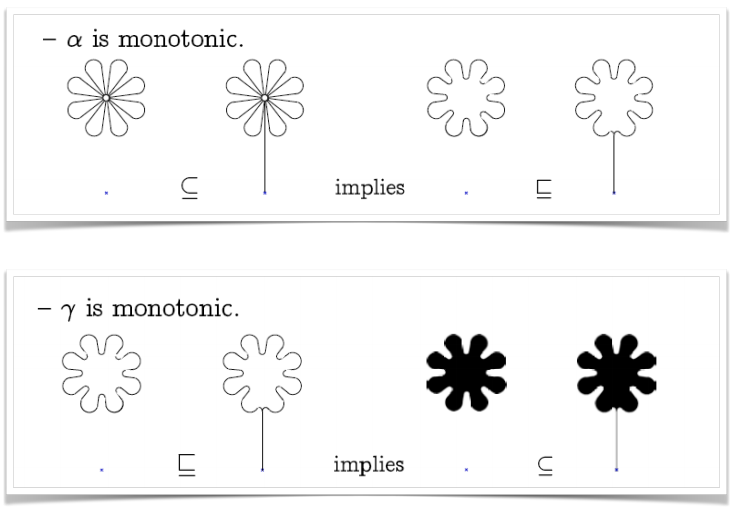
\includegraphics[width=\textwidth, height=\textheight, keepaspectratio]{galConn1.png}
		\caption{Relazioni tra oggetti concreti/astratti}
	\end{subfigure}
	\hfill
	\begin{subfigure}{0.49\textwidth}
	    \centering
		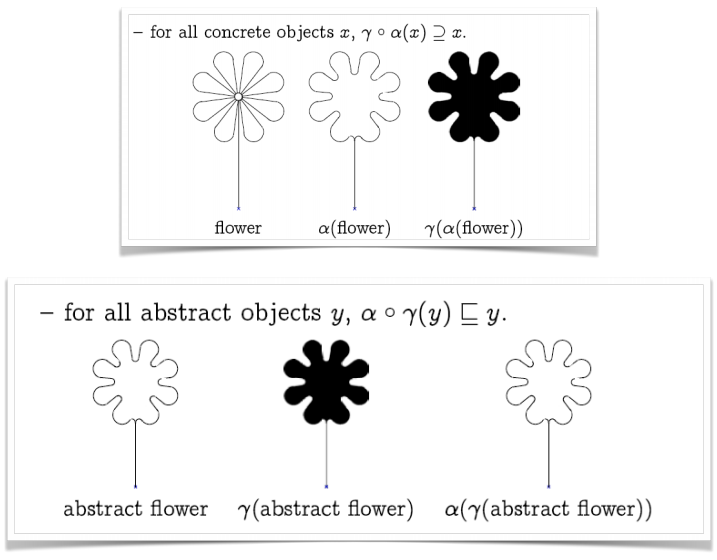
\includegraphics[width=0.9\textwidth]{galConn2.png} 
		\caption{Monotonia}
	\end{subfigure}
\end{figure}

\subsection{Ordinamento e operazioni nel mondo astratto}
Un oggetto astratto è più piccolo ($\sqsubseteq$) di un altro oggetto astratto se ha meno errore. La rappresentazione astratta sarà quindi più precisa e contenuta ($\subseteq$) in quella meno precisa. Con l'aggiunta di questo \textit{ordinamento} posso trasferire le \textit{operazioni} nel mondo astratto. Ad esempio, per l'aggiunta dello stelo (funzione $stem$) prendo l'oggetto astratto, lo concretizzo, applico l'operazione concreta e poi astraggo di nuovo. Per le altre operazioni la tecnica è analoga.
\begin{figure}[htp]
	\begin{subfigure}{0.49\textwidth}
	    \centering
		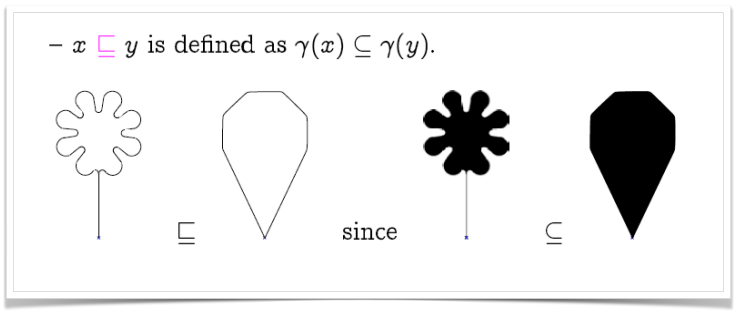
\includegraphics[width=\textwidth, height=\textheight, keepaspectratio]{absOp1.png}
		\caption{Ordinamento nell'astratto}
	\end{subfigure}
	\hfill
	\begin{subfigure}{0.49\textwidth}
	    \centering
		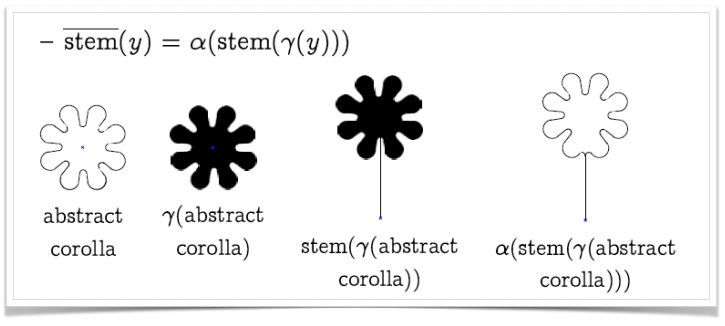
\includegraphics[width=\textwidth, height=\textheight, keepaspectratio]{absOp2.png} 
		\caption{Aggiunta dello stelo nell'astratto}
	\end{subfigure}
\end{figure}


\section{Astrazione delle semantiche} % sezione 2b - slide 26-52
Finora abbiamo definito la \textit{semantica delle tracce}, nel caso discreto, come l'insieme di tutte le possibili esecuzioni di un programma. Siccome tali esecuzioni sono potenzialmente infinite, quello che ci serve è una semantica ancora più astratta che useremo per approssimare la realtà concreta (non decidibile per definizione).

\subsection{Collecting semantics}
Nella collecting semantics, la semantica delle tracce (insieme di tracce) è vista come una \textit{collezione} di tutte le possibili esecuzioni (traccia di insiemi). L'\textit{idea} alla base della collecting semantics è quella di rimuovere la sequenza temporale e mantenere solo le informazioni date dal punto di programma considerato. In sostanza, si tratta di una collezione degli stati che possono apparire su alcune tracce nei diversi punti di programma. Trattandosi di un'\textit{astrazione}, non è più possibile risalire alle tracce di esecuzione del programma. Ad esempio, nella \textit{figura} sottostante, se voglio controllare l'esistenza della traccia rossa, nella semantica delle tracce so che tale evoluzione temporale non è possibile mentre nella collecting semantics non posso saperlo.
\begin{figure}[htp]
	\centering
	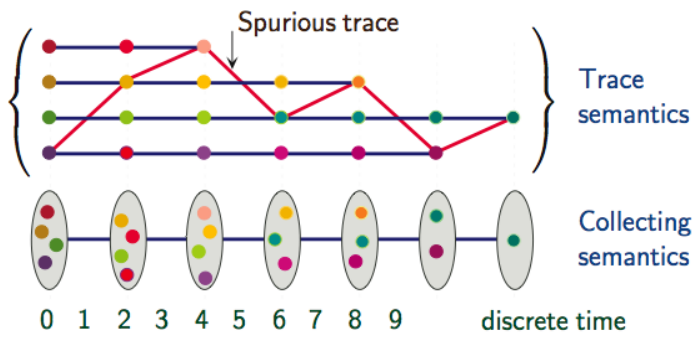
\includegraphics[width=0.9\textwidth]{tr_vs_cs.png}
\end{figure}

\subsection{Esempio di funzionamento}
La collecting semantics differisce dalla semantica delle tracce se nel codice sono presenti dei \textit{cicli}, in quanto per iterazioni successive di tali cicli avrò che la collecting semantics porrà i relativi stati nello stesso insieme (si perde l'ordine temporale degli stati). In sostanza si collezionano gli stati in base a \textit{proprietà simili}. Se paradossalmente avessi degli stati che differiscono tutti gli uni dagli altri, allora raggiungerei un'equivalenza con la semantica delle tracce. Vediamo ora un \textit{esempio di funzionamento}:
\begin{itemize}
    \item Al punto di programma 1 (tempo 0), corrispondente al primo insieme di sinistra, si raggruppano tutti gli stati che compaiono (anche per input differenti).
    \item Al punto di programma 2 comincia un ciclo, perciò il secondo insieme raggrupperà stati con proprietà uguali ad ogni iterazione.
    \item Dal punto di programma 4 si torna a collezionare oggetti nell'insieme creato al punto di programma 2.
    \item Nel quinto insieme si raggruppano gli stati terminali.
\end{itemize}
\begin{figure}[htp]
	\begin{subfigure}{0.49\textwidth}
	    \centering
		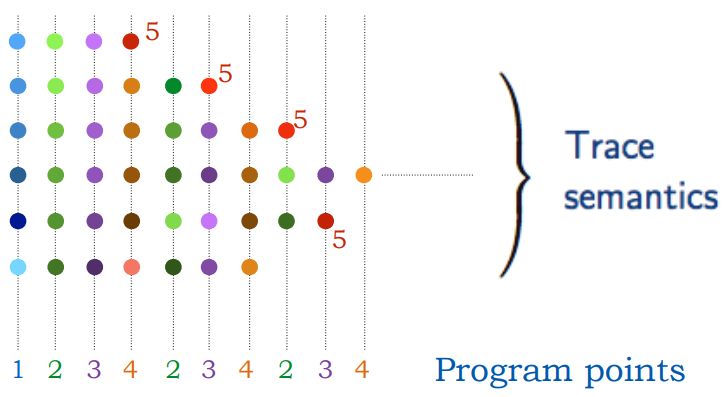
\includegraphics[width=\textwidth, height=\textheight, keepaspectratio]{cs1.png}
		\caption{Punti di programma}
	\end{subfigure}
	\hfill
	\begin{subfigure}{0.49\textwidth}
	    \centering
		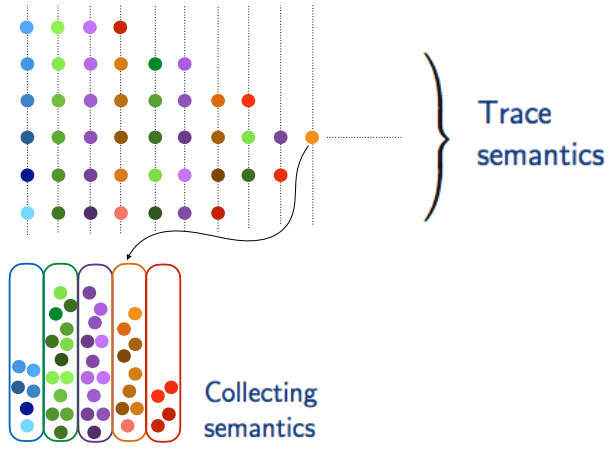
\includegraphics[width=\textwidth, height=\textheight, keepaspectratio]{cs2.png} 
		\caption{Insiemi della collecting semantics}
	\end{subfigure}
\end{figure}

\subsection{Altre notazioni}
Nella \textit{notazione ad intervalli} si applica l'idea di osservare per ogni punto di programma quali sono gli stati che vi ci passano con l'obiettivo di osservare una proprietà che si mantiene nel tempo. Nell'osservazione degli \textit{stati raggiungibili}, invece, non si modella più quando e dove uno stato compare, ma solo se esso viene raggiunto dall'assegnamento di una certa variabile che si sta analizzando.
\begin{figure}[htp]
	\begin{subfigure}{0.49\textwidth}
	    \centering
		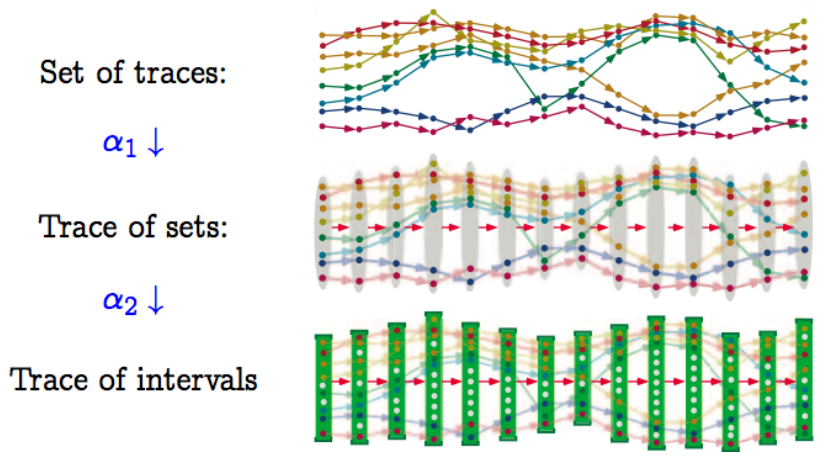
\includegraphics[width=\textwidth, height=\textheight, keepaspectratio]{not1.png}
		\caption{Tracce di intervalli}
	\end{subfigure}
	\hfill
	\begin{subfigure}{0.49\textwidth}
	    \centering
		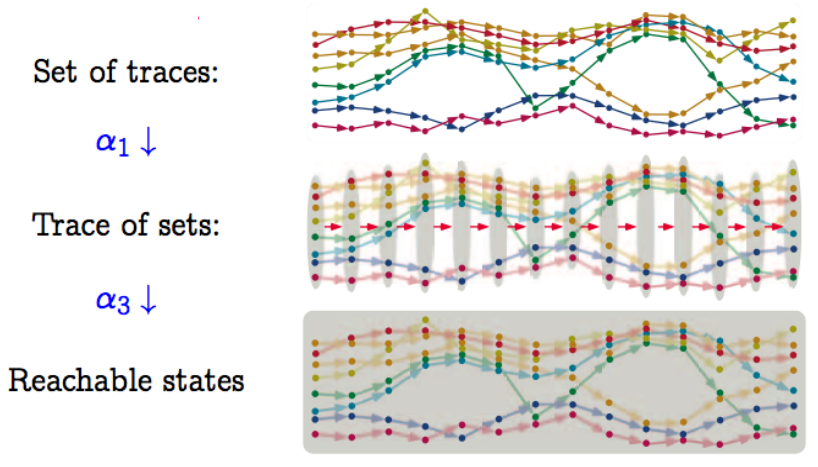
\includegraphics[width=\textwidth, height=\textheight, keepaspectratio]{not2.png} 
		\caption{Stati raggiungibili}
	\end{subfigure}
\end{figure}


\chapter{Interpretazione astratta}

\section{Introduzione} % sezione 2c - slide 2-19
\subsection{Astrazione in base ad una proprietà}
Come abbiamo già detto, l'\textit{astrazione} è un processo molto comune in informatica e consiste nel rappresentare oggetti concreti con descrizioni in cui si considerano solo alcune \textit{proprietà comuni}. Infatti, se considerassimo tutte le proprietà avremmo indecidibilità poiché saremmo ancora nel piano concreto. Definiremo quindi un insieme $A \subseteq \wp(\Sigma)$ come l'insieme degli elementi che vogliamo descrivere in modo preciso con l'astrazione (senza perdita di precisione). Gli elementi al di fuori di $A$ dovranno però essere rappresentati da altri elementi di $A$ (perdita di precisione).

\subsection{Oggetti e proprietà dei programmi}
Quando si analizza un programma, si devono considerare degli \textit{oggetti} che rappresentano gli stati del nostro programma. Tali oggetti possono essere:
\begin{itemize}
    \item Valori (booleani, interi) $\mathcal{V}$.
    \item Nomi delle variabili $\mathbb{X}$.
    \item Ambienti $\mathbb{X} \mapsto \mathcal{V}$.
    \item Stacks.
\end{itemize}
Abbiamo parlato di \textit{proprietà} invarianti come di oggetti in $A$ che hanno tali proprietà. Ora dobbiamo passare da oggetti singoli ad un insieme di oggetti. Possiamo anche vedere un insieme di proprietà $\wp(\Sigma)$ di oggetti in $\Sigma$ (insieme di tutti gli stati) come un \textit{reticolo completo}.
\begin{figure}[htp]
	\begin{subfigure}{0.49\textwidth}
	    \centering
		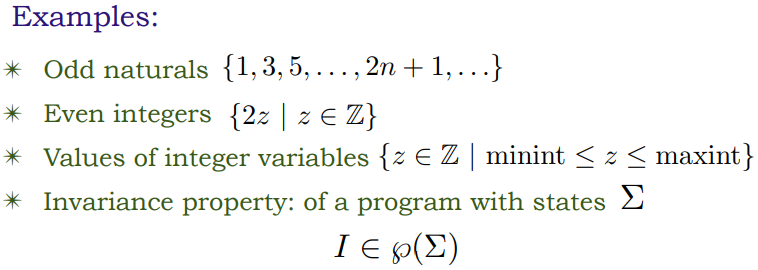
\includegraphics[width=\textwidth, height=\textheight, keepaspectratio]{prop1.png}
		\caption{Esempi di proprietà}
	\end{subfigure}
	\hfill
	\begin{subfigure}{0.49\textwidth}
	    \centering
		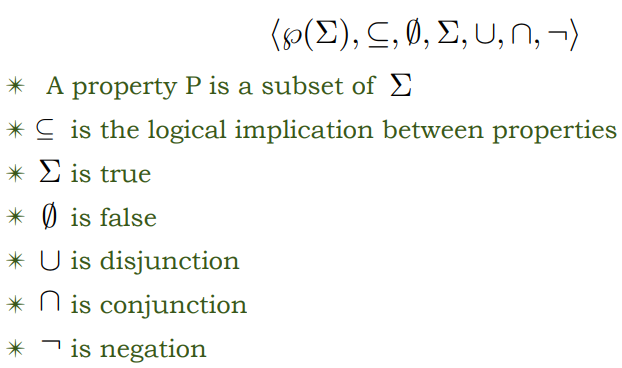
\includegraphics[width=\textwidth, height=\textheight, keepaspectratio]{prop2.png} 
		\caption{Reticolo delle proprietà}
	\end{subfigure}
\end{figure}
\newpage

\subsection{Direzione dell'astrazione}
Quando approssimo una proprietà concreta $P$ in una proprietà astratta $\overline{P}$ posso avere due casi: approssimazione per difetto $\overline{P} \subseteq P$ o approssimazione per eccesso $\overline{P} \supseteq P$ (in cui aggiungo del rumore). Nel caso dell'\textit{approssimazione per difetto}, per stimare se un oggetto ha una proprietà $P$ non decidibile devo stimare un sottoinsieme della proprietà originale $\overline{P}$:
\begin{itemize}
    \item Se $\overline{P}$ non vale per un generico punto, allora non so dire nulla.
    \item Se $\overline{P}$ vale, allora vale anche $P$.
\end{itemize}
Nel caso dell'\textit{approssimazione per eccesso}, invece, ho una proprietà $\overline{P}$ che sovrastima $P$ e quindi posso solo dire se un generico punto non ha la proprietà:
\begin{itemize}
    \item Se $\overline{P}$ non vale, allora sicuramente non vale nemmeno $P$.
    \item Se $\overline{P}$ vale, allora non so dire nulla.
\end{itemize}
Infine ricordiamo che quando si approssima attraverso una rappresentazione astratta si crea un insieme di oggetti \textit{più grande}.
\begin{figure}[htp]
	\begin{subfigure}{0.49\textwidth}
	    \centering
		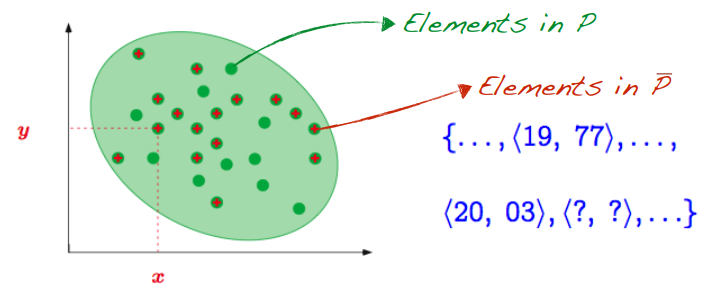
\includegraphics[width=\textwidth, height=\textheight, keepaspectratio]{below.png}
		\caption{Approssimazione per difetto}
	\end{subfigure}
	\hfill
	\begin{subfigure}{0.49\textwidth}
	    \centering
		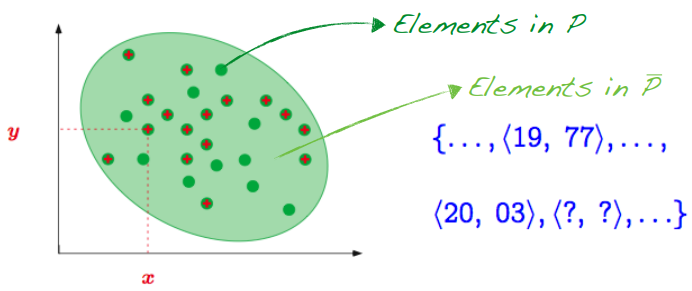
\includegraphics[width=\textwidth, height=\textheight, keepaspectratio]{above.png} 
		\caption{Approssimazione per eccesso}
	\end{subfigure}
\end{figure}

\subsection{Approssimazione minima}
Assumiamo che una proprietà concreta $P$ debba essere approssimata per eccesso da una proprietà $\overline{P}$ tale che $\overline{P} \supseteq P$. L'\textit{approssimazione minima} sarà l'approssimazione ottimale per $P$. Notiamo infatti che non è detto che esista una sola approssimazione per $P$. Inoltre, tali proprietà astratte potrebbero anche essere confrontabili, e quindi si dovrà scegliere quella che aggiunge la minor quantità di rumore.

\subsection{Migliore approssimazione}
Una buona scelta per l'astrazione di una proprietà $P \in A$ consiste nella \textit{migliore approssimazione} delle sue sovra-approssimazioni $\overline{P} \supseteq P$.
\[
    \forall \overline{P}' \in A. \, (P \subseteq \overline{P}') \Rightarrow (\overline{P} \subseteq \overline{P}')
\]
Si può dimostrare che la migliore approssimazione è il \textit{glb} (greatest lower bound) di tutte le approssimazioni, ovvero l'intersezione tra tutte le diverse rappresentazioni astratte.
\[
    \overline{P} = \bigcap \{ \overline{P}' \in A \, | \, P \subseteq \overline{P}' \} \in A
\]

\subsection{Esempio sulla rappresentazione del segno}
Quello che vogliamo rappresentare sono le proprietà delle moltiplicazioni e delle addizioni tra interi. In particolare, la proprietà che dobbiamo studiare è il \textit{segno}. Quindi gli oggetti del dominio astratto saranno:
\begin{itemize}
    \item Gli interi positivi, zero compreso (notazione $+$).
    \item Gli interi negativi, zero compreso (notazione $-$).
    \item Il singoletto $\{ 0 \}$ (notazione $0$).
\end{itemize}
Si può dimostrare che il dominio astratto del segno è \textit{isomorfo} all'insieme delle parti di $\mathbb{Z}$. Da ciò deriviamo che ogni oggetto può essere approssimato come appartenenza ad un insieme in cui si tiene solo il segno (ma si perde il valore). Nella \textit{figura (b)} sottostante viene mostrata l'interpretazione dell'addizione e della moltiplicazione nel nuovo dominio astratto (la notazione $\mathbb{Z}$ indica che non so dire nulla).
\begin{figure}[htp]
	\begin{subfigure}{0.49\textwidth}
	    \centering
		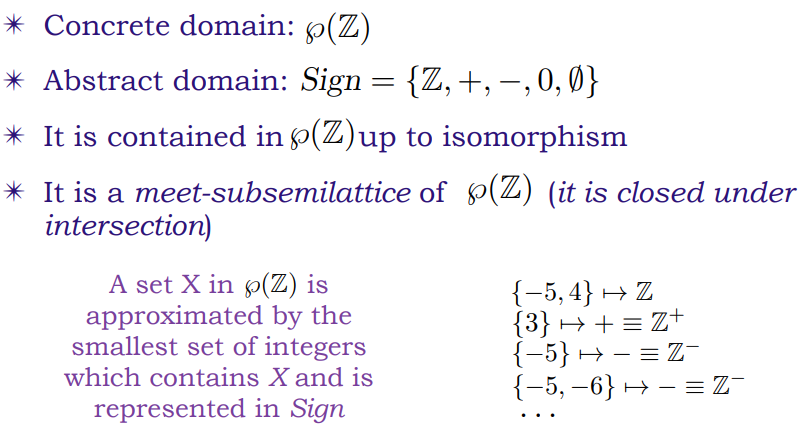
\includegraphics[width=\textwidth, height=\textheight, keepaspectratio]{sign1.png}
		\caption{Dominio concreto e astratto}
	\end{subfigure}
	\hfill
	\begin{subfigure}{0.49\textwidth}
	    \centering
		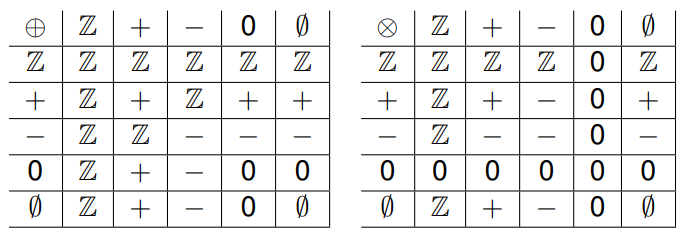
\includegraphics[width=\textwidth, height=\textheight, keepaspectratio]{sign2.png} 
		\caption{Approssimazione degli operatori}
	\end{subfigure}
\end{figure}

\noindent
Infine, possiamo avere anche \textit{altri tipi} di rappresentazioni astratte come per esempio: rettangoli (o intervalli), ottagoni, poliedri, studio delle congruenze.
\begin{figure}[htp]
	\centering
	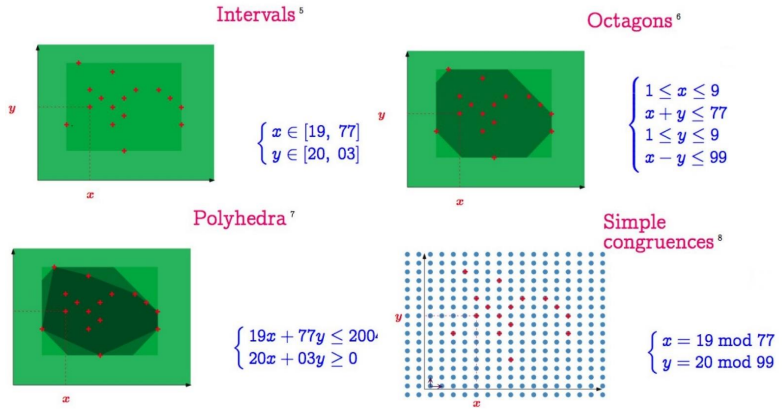
\includegraphics[width=0.5\textwidth]{sign3.png}
\end{figure}


\section{Connessioni di Galois} % sezione 2c - slide 20-34
Per garantire l'esistenza della migliore approssimazione, occorre descrivere matematicamente la \textit{relazione} tra il mondo concreto e quello astratto. Abbiamo già visto che esistono due funzioni $\alpha$ e $\gamma$, dette funzioni di astrazione e concretizzazione, che garantiscono l'esistenza della migliore approssimazione (sugli insiemi ordinati $A$ e $C$). Possiamo dire che esse formano una \textit{connessione di Galois} se:
\begin{itemize}
    \item $\alpha$ e $\gamma$ stesse sono monotone.
    \item $\forall a \in A , c \in C. \, \alpha(c) \leq_A a \iff c \leq_C \gamma(a)$.
\end{itemize}
Una connessione di Galois (GC) si scrive come:
\[
    (C, \leq_C) \galois{\alpha}{\gamma} (A, \leq_A)
\]
dove la funzione $\alpha$ è detta \textit{aggiunta sinistra}, mentre la funzione $\gamma$ è detta \textit{aggiunta destra}. Inoltre, la connessione di Galois tra due domini è \textit{univoca} (se due oggetti hanno la stessa $\alpha$ allora hanno anche la stessa $\gamma$ e viceversa) e quindi le funzioni $\alpha$ e $\gamma$ sono identificabili attraverso:
\[
    \alpha(c) = \bigwedge \{ a \in A \, | \, c \leq_C \gamma(a) \}
\]
\[
    \gamma(a) = \bigvee \{ c \in C \, | \, \alpha(c) \leq_A a \}
\]

\subsection{Esempio}
Supponiamo di avere due insiemi $A$ e $B$ in relazione tra loro mediante $R \subseteq A \times B$. Indichiamo con $A'$ l'approssimazione di $A$, cioè l'astrazione che contiene tutti gli elementi di $B$ che sono in relazione con tutti gli elementi di $A'$. Analogamente, indichiamo con $B'$ l'approssimazione di $B$, cioè l'astrazione che contiene tutti gli elementi di $A$ che sono in relazione con tutti gli elementi di $B'$. Nella \textit{figura} sottostante viene mostrata una rappresentazione grafica in cui si utilizzano gli insiemi $A = \{ 1,3,5 \}$ e $B = \{ 2,4,6 \}$ e come relazione l'essere \textit{minore di}.
\begin{figure}[htp]
	\centering
	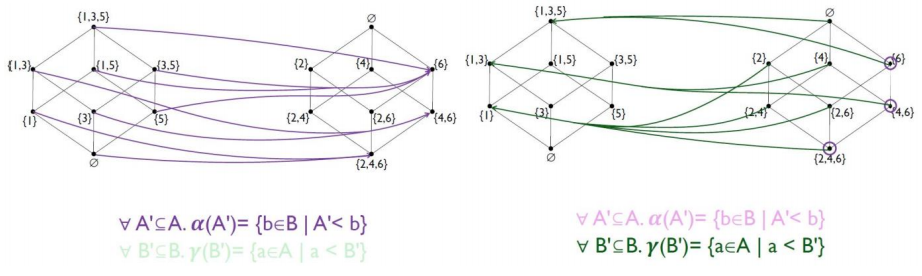
\includegraphics[width=\textwidth, height=\textheight, keepaspectratio]{galConn3.png}
\end{figure}


\section{Inserzioni di Galois} % sezione 2c - slide 35-39
Una connessione di Galois in cui vale che $\alpha \gamma(a) = a$ (identità) si dice \textit{inserzione di Galois}. In questo caso l'astrazione è \textit{suriettiva} per cui ho che più elementi vanno nello stesso valore concreto; e inoltre, la concretizzazione è
\textit{iniettiva} perché un valore concreto è anche la sua concretizzazione. Una inserzione di Galois (GI) si scrive come:
\[
    (C, \leq_C) \galoiS{\alpha}{\gamma} (A, \leq_A)
\]

\subsection{Esempio}
Se nella concretizzazione di un valore astratto ho un solo valore concreto rappresentato, posso rimuovere i valori astratti ridondanti (per la suriettività) e unirli insieme in gruppi creando le inserzioni di Galois.
\begin{figure}[htp]
	\begin{subfigure}{0.49\textwidth}
	    \centering
		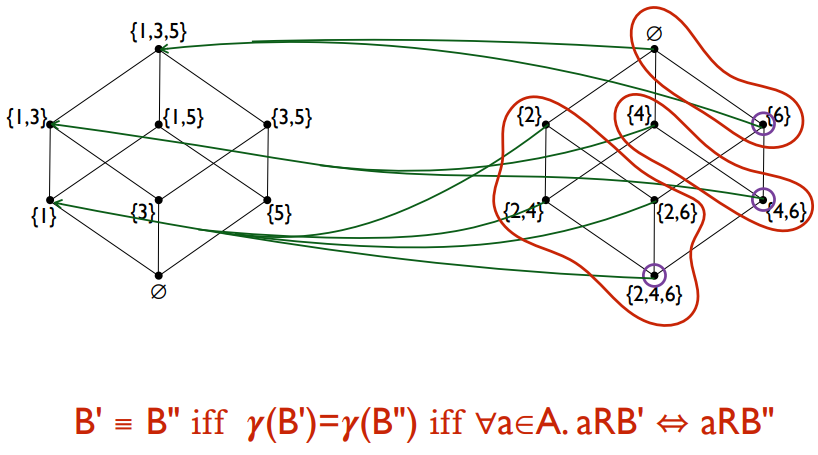
\includegraphics[width=\textwidth, height=\textheight, keepaspectratio]{GCvsGI.png}
		\caption{GC vs GI}
	\end{subfigure}
	\hfill
	\begin{subfigure}{0.49\textwidth}
	    \centering
		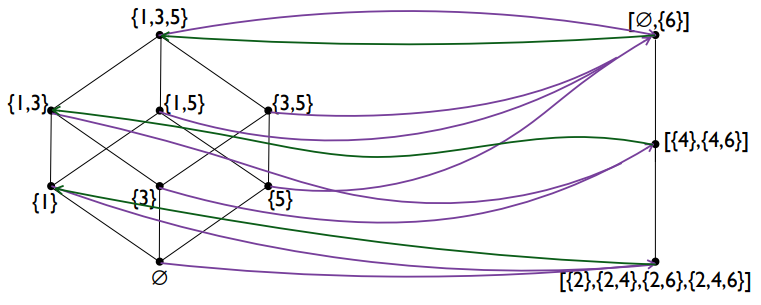
\includegraphics[width=\textwidth, height=\textheight, keepaspectratio]{GI.png} 
		\caption{GI (dominio astratto)}
	\end{subfigure}
\end{figure}


\section{Operatori di chiusura superiore (uco)} % sezione 2c - slide 40-44
Rappresentano un'ulteriore modalità di rappresentazione astratta. Una funzione $\rho: C \rightarrow C$ è un upper closure operator (\textit{uco}) se soddisfa le seguenti proprietà:
\begin{itemize}
	\item Estensività, $\forall x \in C. \, \rho(x) \geq x$
	\item Monotonia, $\forall x,y \in C. \, x \leq y \Rightarrow \rho(x) \leq \rho(y)$
	\item Idempotenza, $\forall x \in C. \, \rho \rho(x) = \rho(x)$
\end{itemize}
Nelle connessioni di Galois (o nelle inserzioni di Galois) $\gamma \alpha$ è un uco.

\subsection{Esempio}
Le \textit{GI} associano ad ogni elemento concreto la proprietà astratta rappresentata fuori dal concreto, mentre gli \textit{uco} associano ad ogni elemento concreto la proprietà astratta come suo significato dentro il concreto. Nella \textit{figura} sottostante viene mostrato un esempio di uco (a sinistra) ottenuto partendo da una GI (a destra).
\begin{figure}[htp]
	\centering
	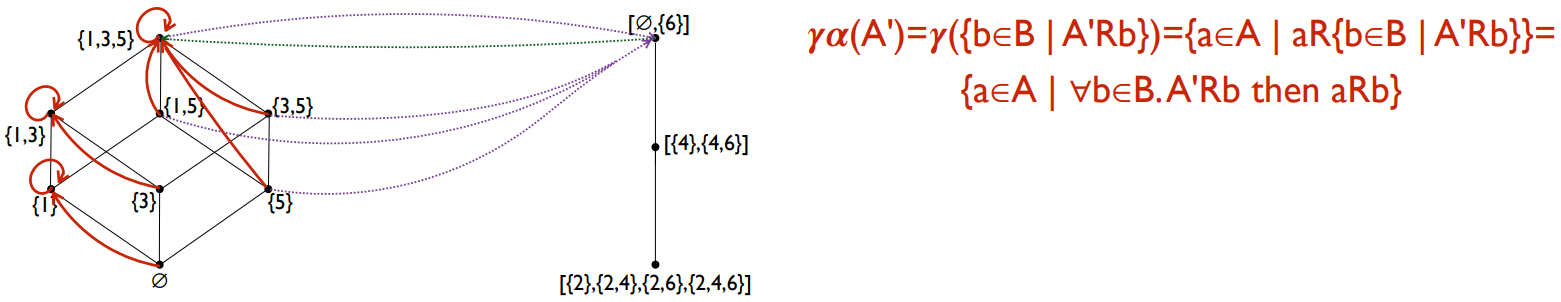
\includegraphics[width=\textwidth, height=\textheight, keepaspectratio]{uco.png}
\end{figure}


\section{Famiglie di Moore} % sezione 2c - slide 45-50
Sia $L$ un reticolo completo. $X \subseteq L$ è una \textit{famiglia di Moore} di $L$ se:
\[
    X = \mathcal{M}(X) = \left\{ \bigwedge S \, | \, S \subseteq X \right\}
\]
dove $\bigwedge \varnothing = \top \in \mathcal{M}(X)$. Da questa definizione segue che essere una famiglia di Moore garantisce l'esistenza della \textit{migliore approssimazione}.

\subsection{Esempio}
\`{E} possibile ricavare le seguenti relazioni:
\begin{itemize}
    \item $C \galoiS{\alpha}{\gamma} A$ è una \textit{GI} se $A$ è isomorfo ad una \textit{Moore family} di $C$ (c'è dipendenza dalla rappresentazione degli elementi).
    \item Se $(C, \leq_C) \galoiS{\alpha}{\gamma} (A, \leq_A)$ è una \textit{GI}, allora $\rho = \gamma \alpha$ è un \textit{uco} (c'è indipendenza dalla rappresentazione degli elementi).
    \item I punti fissi di un \textit{uco} $\rho$ sono una \textit{Moore family} di $C$ (ogni elemento concreto viene astratto nel punto fisso più vicino).
\end{itemize}
\begin{figure}[htp]
	\begin{subfigure}{0.49\textwidth}
	    \centering
		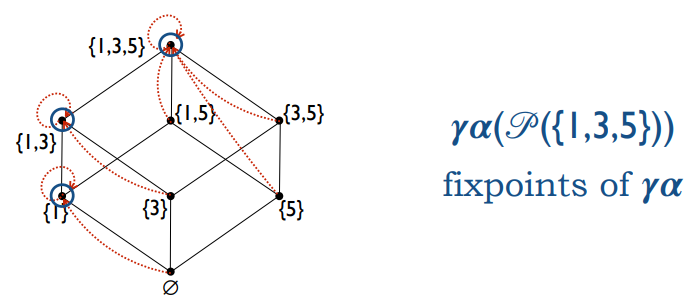
\includegraphics[width=\textwidth, height=\textheight, keepaspectratio]{UCOvsMF.png}
		\caption{Uco vs Moore Families}
	\end{subfigure}
	\hfill
	\begin{subfigure}{0.49\textwidth}
	    \centering
		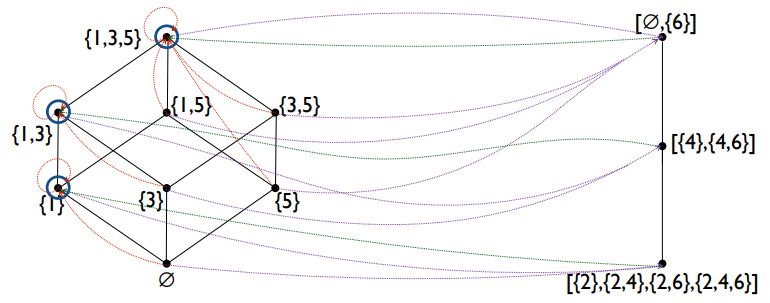
\includegraphics[width=\textwidth, height=\textheight, keepaspectratio]{all.png} 
		\caption{Esempio di riepilogo}
	\end{subfigure}
\end{figure}


\section{Esempio grafico} % sezione 2c - slide 51-55
Facciamo ora un esempio di astrazione e concretizzazione di punti sui numeri reali. Nelle figure i $+$ rappresentano i punti concreti. L'\textit{astrazione} crea quindi degli intervalli in cui ho che $x = [1,99]$ e $y = [2,77]$. Il \textit{significato concreto} è rappresentato dal rettangolo verde in cui considero tutti i possibili punti posti in quegli intervalli. In pratica dagli intervalli, avendo perso la posizione esatta dei punti, passo ad un'area.
\begin{figure}[htp]
	\begin{subfigure}{0.49\textwidth}
	    \centering
		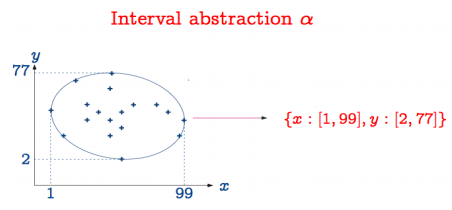
\includegraphics[width=\textwidth, height=\textheight, keepaspectratio]{esAstr.png}
		\caption{Astrazione}
	\end{subfigure}
	\hfill
	\begin{subfigure}{0.49\textwidth}
	    \centering
		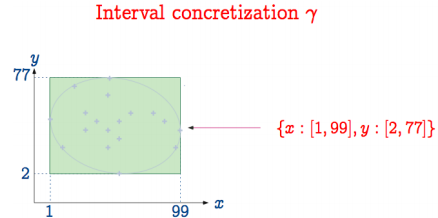
\includegraphics[width=\textwidth, height=\textheight, keepaspectratio]{esConcr.png} 
		\caption{Concretizzazione}
	\end{subfigure}
\end{figure}

\noindent
L'astrazione è \textit{monotona}, ovvero gli intervalli più piccoli sono contenuti in quelli più grandi. La stessa cosa vale anche per la concretizzazione.

Inoltre, la composizione $\gamma \alpha$ è \textit{estensiva} (uco), ovvero mi dice che i punti $+$ sono contenuti nel più piccolo rettangolo che li contiene. Se inverto gli operatori ottengo invece l'\textit{identità}, ovvero se applico l’astrazione dopo la concretizzazione ($\alpha \gamma$) rimango negli intervalli e quindi non ricavo informazione.
\begin{figure}[htp]
    \begin{subfigure}{0.49\textwidth}
        \centering
		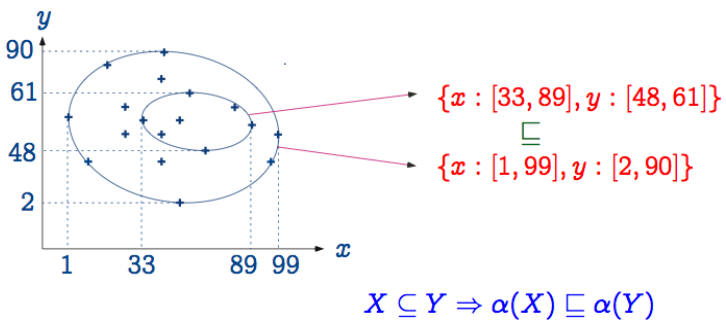
\includegraphics[width=\textwidth, height=\textheight, keepaspectratio]{esMonAstr.png}
		\caption{Monotonia dell'astrazione}
	\end{subfigure}
	\hfill
	\begin{subfigure}{0.49\textwidth}
	    \centering
		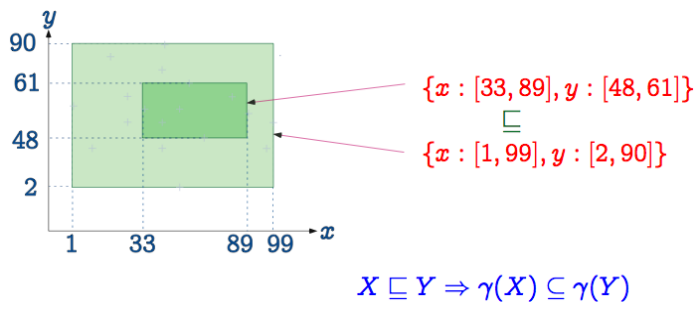
\includegraphics[width=\textwidth, height=\textheight, keepaspectratio]{esMonConcr.png} 
		\caption{Monotonia della concretizzazione}
	\end{subfigure}
	\begin{subfigure}{0.49\textwidth}
	    \centering
		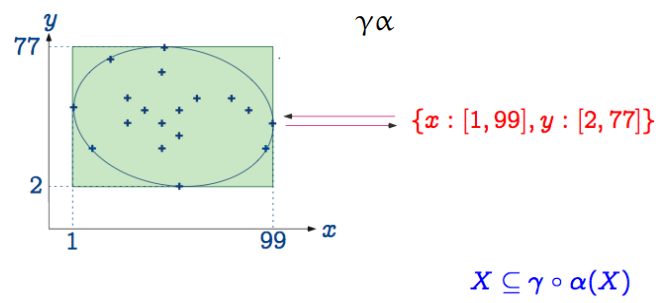
\includegraphics[width=\textwidth, height=\textheight, keepaspectratio]{esEst.png}
		\caption{Estensività}
	\end{subfigure}
	\hfill
	\begin{subfigure}{0.49\textwidth}
	    \centering
		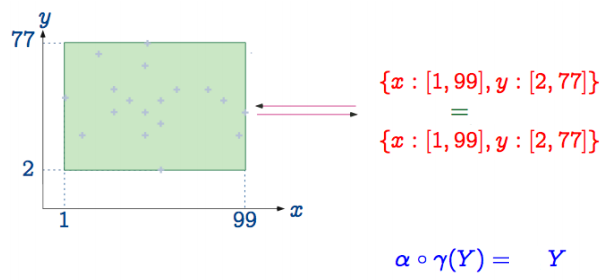
\includegraphics[width=\textwidth, height=\textheight, keepaspectratio]{esId.png} 
		\caption{Identità}
	\end{subfigure}
\end{figure}


\section{Reticolo delle astrazioni} % sezione 2c - slide 56-60
Se $< C, \leq, \wedge, \vee, \bot, \top >$ è un reticolo completo, allora
\[
    < uco(C), \sqsubseteq, \sqcap, \sqcup, \lambda x.\top, \lambda x.x >
\]
è un reticolo completo in cui vengono soddisfatte le seguenti proprietà:
\begin{itemize}
	\item \textit{Confronto} tra domini astratti (grado di precisione) $A_1 \sqsubseteq A_2$
	\[
	    \rho \sqsubseteq \eta \Leftrightarrow \forall y \in C. \, \rho(y) \leq \eta(y) \Leftrightarrow \eta(C) \subseteq \rho(C)
	\]
	\item \textit{GLB} di astrazioni $\bigsqcap_i A_i$
	\[
	    \left( \bigsqcap_{i \in I} \rho_i \right) (x) = \bigwedge_{i \in I} \rho_i (x)
    \]
	\item \textit{LUB} di astrazioni $\bigsqcup_i A_i$
	\[
        \left( \bigsqcup_{i \in I} \rho_i \right) (x) = x \Leftrightarrow \forall i \in I. \, \rho_i (x) = x
    \]
	\item Astrazione \textit{più astratta} (imprecisa), ovvero il dominio $\{ \top \}$
	\[
	    \lambda x.\top
    \]
	\item Astrazione \textit{più concreta} (precisa), ovvero il dominio identità $C$
	\[
	    \lambda x.x
    \]
\end{itemize}


\section{Computazioni astratte e concrete} % sezione 2c - slide 61-71
Finora abbiamo visto come costruire i domini astratti, ma il nostro obiettivo è quello di spostare la \textit{computazione} da un mondo concreto non decidibile ad un mondo astratto decidibile.

\subsection{Correttezza (soundness)}
Consideriamo una GI $C \galoiS{\alpha}{\gamma} A$, una funzione concreta $f: C \rightarrow C$ e una funzione astratta $f^{\sharp}: A \rightarrow A$. Possiamo dire che $f^{\sharp}$ è un'\textit{approssimazione corretta} (sound) di $f$ in $A$ se:
\[
	\forall x \in C. \, \alpha(f(x)) \leq f^{\sharp}(\alpha(x))
    \Leftrightarrow
	\forall x \in A. \, f(\gamma(x)) \leq \gamma(f^{\sharp}(x))
\]
Come conseguenza abbiamo che:
\[
	\forall x \in C. \, \alpha(f(x)) \leq f^{\sharp}(\alpha(x))
    \Leftrightarrow
	\forall x \in A. \, \alpha(f(\gamma(x))) \leq f^{\sharp}(x)
\]
e quindi $\alpha \circ f \circ \gamma: A \rightarrow A$ è la \textit{best correct approximation} (bca) di $f$ in $A$.
\begin{figure}[htp]
	\begin{subfigure}{0.49\textwidth}
	    \centering
		\includegraphics[width=\textwidth, height=\textheight, keepaspectratio]{sound1.png}
		\caption{Correttezza (nelle astrazioni)}
	\end{subfigure}
	\hfill
	\begin{subfigure}{0.49\textwidth}
	    \centering
		\includegraphics[width=\textwidth, height=\textheight, keepaspectratio]{sound2.png} 
		\caption{Correttezza (nelle chiusure)}
	\end{subfigure}
\end{figure}

\subsection{Completezza (precision)}
Quando rafforziamo le condizioni di correttezza richiedendo l'uguaglianza otteniamo due nozioni di \textit{completezza} incomparabili. Infatti, se consideriamo una GI $C \galoiS{\alpha}{\gamma} A$, una funzione concreta $f: C \rightarrow C$ e una funzione astratta $f^{\sharp}: A \rightarrow A$, allora potremo dire che:
\begin{itemize}
	\item $f^{\sharp}$ è \textit{backward-complete} se $\forall x \in C. \, \alpha(f(x)) = f^{\sharp}(\alpha(x))$.
	\item $f^{\sharp}$ è \textit{forward-complete} se $\forall x \in A. \, f(\gamma(x)) = \gamma(f^{\sharp}(x))$.
\end{itemize}
Le definizioni di completezza possono essere date anche usando gli \textit{uco}:
\begin{itemize}
	\item $\rho \in uco(C)$ è \textit{backward-complete} se $\rho \circ f = \rho \circ f \circ \rho$.
	\item $\rho \in uco(C)$ è \textit{forward-complete} se $f \circ \rho = \rho \circ f \circ \rho$.
\end{itemize}
\begin{figure}[htp]
	\begin{subfigure}{0.49\textwidth}
	    \centering
		\includegraphics[width=\textwidth, height=\textheight, keepaspectratio]{complete1.png}
		\caption{Completezza (nelle astrazioni)}
	\end{subfigure}
	\hfill
	\begin{subfigure}{0.49\textwidth}
	    \centering
		\includegraphics[width=\textwidth, height=\textheight, keepaspectratio]{complete2.png} 
		\caption{Completezza (nelle chiusure)}
	\end{subfigure}
\end{figure}

\subsection{Forward vs Backward}
I due tipi di completezza rappresentano una situazione ideale in cui non si verifica alcuna perdita di precisione durante l'astrazione. In particolare:
\begin{itemize}
	\item La \textit{Backward-completezza} considera l'astrazione sull'output delle operazioni (non si accumula alcuna perdita di precisione astraendo in $\rho$ gli argomenti di $f$).
	\item La \textit{Forward-completezza} considera l'astrazione sull'input delle operazioni (non si accumula alcuna perdita di precisione approssimando il risultato della funzione $f$ calcolata in $\rho$).
\end{itemize}

\subsection{Esempio su intervalli di interi} % sezione 2c - slide 72-74
Consideriamo un dominio composto da certi \textit{intervalli di interi} (con distinzione tra positivi e negativi). I pallini rossi sono gli intervalli che formano la \textit{rappresentazione astratta} degli intervalli concreti. La funzione $f$ che dovremo calcolare è il quadrato. La \textit{proprietà astratta} sarà quindi rappresentata da tutti i valori positivi, poiché i valori negativi al quadrato confluiscono in quelli positivi. Il \textit{primo insieme} di pallini rossi considerato $\{ \mathbb{Z}, [0,+\infty], [0,10] \}$ è Forward ma non Backward completo, in particolare:
\begin{itemize}
    \item \`{E} \textit{forward-complete} perché per ogni elemento vale che $f \circ \rho = \rho \circ f \circ \rho$, ovvero se seguo $f$ in avanti cado sempre dentro l'insieme.
    \item Non è \textit{backward-complete} perché $\rho \circ f ([0,2]) \neq \rho \circ f \circ \rho ([0,2])$, ovvero esiste almeno un elemento che entra dentro ma che si trova fuori dall'insieme (se seguo $f$ all'indietro cado fuori dall'insieme).
\end{itemize}
Il \textit{secondo insieme} di pallini rossi considerato $\{ \mathbb{Z}, [0,2], [0,0] \}$ è Backward ma non Forward completo, in particolare:
\begin{itemize}
    \item \`{E} \textit{backward-complete} perché se seguo $f$ all'indietro dai pallini rossi non esco mai dall'insieme (in questo insieme solo $[0,0]$ può seguire $f$ all'indietro e infatti rimane dentro).
    \item Non è \textit{forward-complete} perché esiste almeno un elemento tale per cui se seguo $f$ in avanti da esso esco dall'insieme.
\end{itemize}
\begin{figure}[htp]
	\begin{subfigure}{0.49\textwidth}
	    \centering
		\includegraphics[width=\textwidth, height=\textheight, keepaspectratio]{intervals1.png}
		\caption{Primo insieme}
	\end{subfigure}
	\hfill
	\begin{subfigure}{0.49\textwidth}
	    \centering
		\includegraphics[width=\textwidth, height=\textheight, keepaspectratio]{intervals2.png} 
		\caption{Secondo insieme}
	\end{subfigure}
\end{figure}


\section{Estrapolazione del punto fisso} % sezione 2c - slide 75-79
In generale, è impossibile calcolare la \textit{semantica del punto fisso} mediante astrazione $\alpha(\text{lfp} F)$ senza calcolare $\text{lfp} F$. La cosa più semplice da fare sarebbe definire $\overline{F}$, sul dominio astratto, tale che $\alpha(\text{lfp} F) = \text{lfp} \overline{F}$. Sfortunatamente però, $\overline{F}$ non è in genere stimabile nel concreto. Inoltre, anche se siamo nel dominio astratto, non è garantita la \textit{convergenza} in quanto l'astrazione cerca di risolvere il problema della decidibilità ma non è detto che risolva quello della convergenza. Nella \textit{figura (a)} sottostante notiamo infatti la presenza di catene ascendenti divergenti a valori infiniti. Ciò significa che non esiste un punto fisso (non è calcolabile). Analizziamo infine la \textit{figura (b)}:
\begin{itemize}
    \item L'insieme di sinistra (in verde) corrisponde ai \textit{punti pre-fissi}.
    \item L'insieme di destra (in azzurro) corrisponde ai \textit{punti post-fissi}.
    \item Con il \textit{widening} si accelera il calcolo del punto fisso spostandosi nel calcolo dei punti post-fissi.
    \item Con il \textit{narrowing} si cerca la migliore approssimazione del punto fisso raffinando i punti post-fissi.
\end{itemize}
\begin{figure}[htp]
	\begin{subfigure}{0.49\textwidth}
	    \centering
		\includegraphics[width=\textwidth, height=\textheight, keepaspectratio]{fpEx1.png}
		\caption{Catene ascendenti infinite}
	\end{subfigure}
	\hfill
	\begin{subfigure}{0.49\textwidth}
	    \centering
		\includegraphics[width=\textwidth, height=\textheight, keepaspectratio]{fpEx2.png} 
		\caption{Immagine riassuntiva}
	\end{subfigure}
\end{figure}


\chapter{Analisi statica}

\section{Introduzione} % sezione 3 - slide 1-7
L'\textit{analisi statica} studia le proprietà del programma (senza eseguirlo). Tali \textit{proprietà} devono però essere astratte, per poter far rispondere l'analizzatore in modo decidibile. L'obiettivo sarà quindi quello di dire se una certa \textit{semantica} soddisfa o meno una proprietà astratta. L'analisi statica può essere utile per cercare di prevedere il comportamento di un programma a livello di esecuzione o per ottimizzare il programma stesso (riduzione della lunghezza, eliminazione di parti non raggiungibili).

\subsection{Analisi sul CFG} % sezione 3 - slide 8-27
L'analisi statica si basa sull'analisi della semantica. Un possibile approccio è quello di analizzare il \textit{flusso di controllo} servendosi del CFG. Per l'\textit{analisi sul CFG} viene quindi generato un grafo per ogni procedura. Poi, le analisi che vengono eseguite sono localizzate su tre livelli:
\begin{enumerate}
    \item \textit{Locali} al blocco, cioè eseguite all'interno di uno stesso basic block.
    \item \textit{Intra-procedurali}, che considerano il flusso di informazioni in un singolo CFG.
    \item \textit{Inter-procedurali}, che considerano il flusso di informazioni in un programma visto come un insieme di vari CFG.
\end{enumerate}
Nell'analisi sul CFG si studia come l'informazione viene modificata all'interno di un blocco di istruzioni. L'informazione è caratterizzata dalla soluzione dell'\textit{equazione di punto fisso} che viene definita per ogni blocco. In alcuni casi questa equazione si ottiene dai seguenti tre passaggi:
\begin{enumerate}
    \item Caratterizzare l'\textit{informazione entrante} in un blocco come la combinazione di tutto ciò che esce dai blocchi precedenti.
    \item Caratterizzare l'\textit{informazione uscente} dal blocco come l'informazione entrante modificata dalle operazioni eseguite nel blocco.
    \item \textit{Combinazione} delle definizioni precedenti nell'equazione di punto fisso.
\end{enumerate}


\section{Available Expressions}
\label{avail1}
Potremmo essere interessati a controllare se un'espressione di un assegnamento non cambia nel tempo. In questo modo si potrebbe evitare di \textit{ricalcolare} l'espressione successivamente, ovvero quando essa viene assegnata ad un'altra variabile. Dovremo quindi verificare se l'espressione $e$ è disponibile (\textit{available}) nella variabile $x$ al punto di programma $p$. Per fare questo bisogna controllare che:
\begin{itemize}
    \item $e$ sia stata valutata in un punto di programma precedente a $p$.
    \item Il risultato di $e$ sia stato assegnato a $x$.
    \item Sia $x$ che le variabili in $e$ non devono essere state modificate tra la valutazione e $p$.
\end{itemize}
\begin{figure}[htp]
	\begin{subfigure}{0.49\textwidth}
	    \centering
		\includegraphics[width=0.55\textwidth]{availExp1.png}
		\caption{Ricalcolo di un'espressione}
	\end{subfigure}
	\hfill
	\begin{subfigure}{0.49\textwidth}
	    \centering
		\includegraphics[width=\textwidth, height=\textheight, keepaspectratio]{availExp2.png} 
		\caption{Available expression su un cammino}
	\end{subfigure}
\end{figure}

\subsection{Costruire le equazioni}
\label{avail2}
Le \textit{equazioni} da costruire sono:
\begin{align*}
    AvailOut(n) &= Gen(n) \cup (AvailIn(n) \setminus Kill(n)) \\
    AvailIn(n) &= 
    	\begin{cases}
    		\varnothing & se \, n=entry \\
    		\bigcap_{p \in pred(n)} AvailOut(p) & altrimenti
    	\end{cases} \\
    Gen(p) &= \{ x \leftarrow e \in p \, | \, x \notin Var(e) \} \\
    Kill(p) &= \{ x \leftarrow e \, | \, \exists y \leftarrow e' \in p. \, y \in Var(e) \cup \{ x \} \}
\end{align*}
Manipolandole possiamo ottenere la seguente \textit{equazione di punto fisso}:
\[ AvailIn(n) = \bigcap_{p \in pred(n)} Gen(p) \cup (AvailIn(p) \setminus Kill(p)) \]
$AvailIn$ rappresenta le espressioni disponibili all'ingresso del blocco e viene calcolato come intersezione sui predecessori di quello che generano i predecessori unito a quello che viene tramandato invariato tra predecessori meno l'informazione ridotta man mano dai vari blocchi. 

\subsection{Risolvere il problema}
Per calcolare $AvailIn$ l'analizzatore usa un algoritmo formato da tre passaggi:
\begin{enumerate}
    \item Costruire il CFG.
    \item Raccogliere l'informazione iniziale ($Gen$ e $Kill$).
    \item Risolvere l'equazione di punto fisso.
\end{enumerate}
\begin{figure}[htp]
	\begin{subfigure}{0.49\textwidth}
	    \centering
		\includegraphics[width=\textwidth, height=\textheight, keepaspectratio]{availExp3.png}
		\caption{Raccolta dell'informazione iniziale}
	\end{subfigure}
	\hfill
	\begin{subfigure}{0.49\textwidth}
	    \centering
		\includegraphics[width=\textwidth, height=\textheight, keepaspectratio]{availExp4.png} 
		\caption{Risoluzione dell'equazione}
	\end{subfigure}
\end{figure}

\subsection{Esempio}
\label{avail4}
\begin{figure}[htp]
	\centering
	\includegraphics[width=\textwidth, height=\textheight, keepaspectratio]{availExp5.png}
\end{figure}


\section{Framework monotono} % sezione 3 - slide 28-70
Dobbiamo formalizzare l'\textit{informazione astratta} che vogliamo analizzare. Inoltre, dobbiamo anche definire la funzione di trasferimento astratta (\textit{abstract edge effect}) che rappresenta la semantica operazionale astratta. Dobbiamo poi costruire un \textit{sistema di equazioni} la cui soluzione ci darà l'informazione astratta per ogni punto di programma.

\subsection{Abstract edge effect}
\label{avail3}
Definiamo la semantica astratta nel caso dell'analisi di \textit{available expressions} per ogni etichetta del CFG:
\begin{align*}
    \llbracket ; \rrbracket^\# A &= A \\
    \llbracket NonZero(e) \rrbracket^\# A &= \llbracket Zero(e) \rrbracket^\# A = A \\
    \llbracket input(x) \rrbracket^\# A &= A \\
    \llbracket x \leftarrow e \rrbracket^\# A &=
        \begin{cases}
    		(A \setminus Occ(x)) \cup \{ x \leftarrow e \} & se \, x \notin Var(e) \\
    		A \setminus Occ(x) & altrimenti
    	\end{cases}
\end{align*}
dove $Occ(x) = \{ y \leftarrow e \, | \, x \in Var(e) \cup \{ y \} \}$.

\subsection{Fonti di imprecisione}
Un assegnamento è \textit{disponibile definitivamente} al punto di programma $v$ se è disponibile su tutti i cammini che portano dall'entry a $v$. In sostanza, si intersecano tutte le semantiche dei cammini che arrivano a $v$ partendo dall'entry. La monotonia della funzione di trasferimento garantisce la \textit{terminazione} e quindi il raggiungimento del punto fisso (soundness). Abbiamo però un'\textit{imprecisione} che nasce dal fatto che approssimiamo il programma usando il CFG, il quale rende possibili dei cammini che semanticamente non lo sarebbero. Inoltre, siccome si guarda alla sintassi e non al valore interno, se ho due assegnamenti allo stesso valore (ma con espressioni diverse), non riuscirò a catturare tutte le espressioni disponibili.
\begin{figure}[htp]
	\begin{subfigure}{0.49\textwidth}
	    \centering
		\includegraphics[width=0.9\textwidth]{availExp6.png}
		\caption{Disponibile definitivamente}
	\end{subfigure}
	\hfill
	\begin{subfigure}{0.49\textwidth}
	    \centering
		\includegraphics[width=\textwidth, height=\textheight, keepaspectratio]{availExp7.png} 
		\caption{Imprecisione}
	\end{subfigure}
\end{figure}

\subsection{Esempio}
\label{avail5}
Il \textit{calcolo della soluzione} consiste nel costruire un sistema di disequazioni (una per ogni punto di programma):
\begin{align*}
    \mathcal{A}[entry] &\subseteq \varnothing \\
    \mathcal{A}[v] &\subseteq \llbracket k \rrbracket^\# (\mathcal{A}[u])
\end{align*}
dove $k=(u,lab,v)$. $\mathcal{A}$ rappresenta quindi l'informazione disponibile localmente:
\begin{itemize}
    \item All'entry non ho nulla.
    \item Al punto $v$ ho quello che avevo prima più quello che sopravvive dopo l'esecuzione dell'arco $k$.
\end{itemize}
Per risolvere il sistema di disequazioni si può usare l'algoritmo \textit{Naive} o l'algoritmo \textit{Round-robin}. Nel caso del Round-robin la computazione di un valore utilizza tutti i valori calcolati precedentemente, e quindi anche quelli dell'iterazione corrente, poiché viene mantenuta una struttura dati a cui si accede sia in lettura che in scrittura.
\begin{figure}[htp]
	\begin{subfigure}{0.49\textwidth}
	    \centering
		\includegraphics[width=\textwidth, height=\textheight, keepaspectratio]{availExp8.png}
		\caption{Algoritmo Naive}
	\end{subfigure}
	\hfill
	\begin{subfigure}{0.49\textwidth}
	    \centering
		\includegraphics[width=\textwidth, height=\textheight, keepaspectratio]{availExp9.png} 
		\caption{Algoritmo Round-robin}
	\end{subfigure}
\end{figure}

\subsection{MOP vs MFP}
La \textit{MFP} (Maximum Fixed Point) è la soluzione che combina i valori dell'analisi quando il CFG ha dei nodi in cui convergono due o più percorsi. La soluzione MFP \textit{approssima} la soluzione MOP. Infatti, la \textit{MOP} (Merge Over all Paths) è una soluzione più precisa rispetto alla MFP ($MOP \sqsupseteq MFP$) poiché combina i valori dell'analisi di \textit{tutti i percorsi} del CFG (dopo averli attraversati tutti). La soluzione MOP è quella che vorremmo ma, in generale, essa \textit{non è computabile} in quanto ci possono essere un numero infinito di percorsi. Le soluzioni MOP e MFP coincidono quando tutte le funzioni di trasferimento (abstract edge effect) sono \textit{distributive} ($MOP = MFP$). Dunque se le funzioni di trasferimento sono distributive, è possibile calcolare la soluzione MOP attraverso l'algoritmo iterativo del \textit{punto fisso}.
\begin{figure}[htp]
	\centering
	\includegraphics[width=\textwidth, height=\textheight, keepaspectratio]{MOPvsMFP.png}
\end{figure}

\subsection{Problemi distributivi e non distributivi}
I \textit{problemi distributivi} sono i cosiddetti problemi "semplici", ovvero tutte quelle proprietà che ci dicono \textit{come} un programma viene eseguito. Sono distributive le analisi di:
\begin{itemize}
    \item \textit{Available expressions}.
    \item \textit{Live variables}.
    \item \textit{Reaching definitions}.
    \item \textit{Very busy expressions}.
\end{itemize}
I \textit{problemi non distributivi}, invece, sono quelli che ci dicono \textit{cosa} calcola un programma (ad esempio che l'output è una costante, è un valore positivo, appartiene ad un intervallo eccetera). \`{E} non distributiva l'analisi di \textit{constant propagation}.

\subsection{Sommario}
La \textit{funzione di trasferimento} trasforma ad ogni passo di computazione l'informazione raccolta fino a quel momento. Essa ha due proprietà:
\begin{enumerate}
    \item Include la funzione identità $\forall x \in V. \, I(x) = x$.
    \item \`{E} chiusa rispetto alla composizione.
\end{enumerate}
Per garantire che un algoritmo iterativo abbia una soluzione, bisogna avere funzioni di trasferimento monotone (\textit{framework monotono}). Tale condizione è formalizzata come:
\[ \forall x,y \in V. \, \forall f \in F. \, x \leq y \Rightarrow f(x) \leq f(y) \]
\[ \forall x,y \in V. \, \forall f \in F. \, f(x \wedge y) \leq f(x) \wedge f(y) \]
Tuttavia, alcune volte un framework soddisfa condizioni più restrittive. Infatti, un framework è detto \textit{distributivo} se:
\[ \forall x,y \in V. \, \forall f \in F. \, f(x \wedge y) = f(x) \wedge f(y) \]
L'\textit{algoritmo iterativo} per il calcolo di un'analisi di data-flow è il seguente:
\begin{itemize}
    \item \textit{Input}, un data-flow framework composto da:
    \begin{enumerate}
        \item Un \textit{CFG} (con entry ed exit point).
        \item Un \textit{insieme di valori} $V$ (dominio).
        \item Un'\textit{operazione di combinazione} $\wedge$ (possible/definite).
        \item Un \textit{insieme di funzioni di trasferimento} $F$ tale che $f_B \in F$.
        \item Un \textit{valore costante} di ingresso per entry o exit (forward/backward).
    \end{enumerate}
    \item \textit{Output}, valori in $V$ per $IN[B]$ e $OUT[B]$ per ogni blocco $B$ del CFG (cioè le informazioni in ingresso a $B$ e in uscita da $B$).
\end{itemize}
\begin{figure}[htp]
	\begin{subfigure}{0.49\textwidth}
	    \centering
		\includegraphics[width=\textwidth, height=\textheight, keepaspectratio]{fwAlg.png}
		\caption{Forward data-flow algorithm}
	\end{subfigure}
	\hfill
	\begin{subfigure}{0.49\textwidth}
	    \centering
		\includegraphics[width=\textwidth, height=\textheight, keepaspectratio]{bwAlg.png} 
		\caption{Backward data-flow algorithm}
	\end{subfigure}
\end{figure}
Le \textit{proprietà} dell'algoritmo sono:
\begin{itemize}
    \item Se l'algoritmo converge, il risultato è una possibile soluzione al sistema di equazioni.
    \item Se il framework è monotono, il risultato è la soluzione MFP del sistema di equazioni (ogni altra soluzione del problema sarà sicuramente meno precisa).
    \item Se il framework monotono è un reticolo ACC (ad altezza finita), la convergenza è garantita.
\end{itemize}

\subsection{Soluzione IDEAL}
La \textit{soluzione IDEAL} è la soluzione migliore, ma non è computabile. Infatti a differenza della MOP, la IDEAL prende in considerazione solamente i \textit{percorsi possibili}, ossia quelli che verranno sicuramente attraversati da qualche esecuzione. La soluzione IDEAL calcola quindi i valori alla fine di ogni possibile percorso di esecuzione e ne fa la combinazione. Il problema della non computabilità sta nel fatto che non è possibile conoscere i cammini eseguibili in maniera statica. Qualsiasi soluzione più \textit{piccola} della IDEAL sarà quindi \textit{meno precisa} (safe), anche se convergente, in quanto avrà considerato un numero di vincoli maggiore di quello necessario. Qualsiasi soluzione più \textit{grande} della IDEAL sarà invece \textit{scorretta} (unsound).

\subsection{MOP vs MFP vs IDEAL}
La soluzione MOP prende in considerazione tutti i cammini che dall'entry vanno in un determinato blocco $B$. La \textit{perdita di precisione} sta nel fatto che possono essere considerati anche cammini che non verranno mai eseguiti. Nella MOP avrò quindi i cammini della IDEAL più alcuni cammini spuri ($MOP \sqsubseteq IDEAL$). Combinando queste informazioni con quanto già osservato nel confronto tra MOP e MFP si ottiene la seguente relazione:
\[ MFP \sqsubseteq MOP \sqsubseteq IDEAL \]


\section{Analisi di data-flow} % sezione 3 - slide 71-72
Le \textit{analisi di data-flow} sono analisi che parlano di \textit{come} il programma calcola i valori, ovvero di come i dati evolvono attraverso gli elementi del programma a tempo di esecuzione.


\section{Analisi delle variabili live} % sezione 3 - slide 73-111
\label{live1}
L'analisi delle variabili live è essenziale per l'\textit{allocazione dei registri}. Infatti, due variabili diverse non possono essere salvate nel medesimo registro se sono entrambe in uso. L'\textit{obiettivo} dell'analisi sarà quindi quello di individuare gli intervalli di liveness delle variabili per dire, ad esempio, se nel programma ci sono delle definizioni a vuoto che possono essere rimosse.

\subsection{Variabile live}
Una variabile $x$ è \textit{live} all'uscita del blocco $C$ se verrà usata successivamente. Una variabile $x$ è invece non-live (o \textit{dead}) dopo il blocco $C$ se viene ridefinita prima di un successivo utilizzo. Una variabile $x$ è \textit{live in un cammino} $\pi$ ($v \rightarrow exit$) se:
\begin{itemize}
    \item $\pi$ non contiene definizioni di $x$.
    \item Esiste almeno un uso di $x$ in $\pi$ senza precedenti ridefinizioni di $x$.
\end{itemize}
Possiamo quindi dire che una variabile $x$ è live se si trova tra una definizione ed un uso. Infatti, se decomponiamo il cammino $\pi$ in $\pi = \pi_1 k \pi_2$ abbiamo che: $k$ contiene un uso di $x$; e $\pi_1$ non contiene definizioni di $x$.

\subsection{Esempio su un programma}
Per dire se una variabile è live oppure no bisogna guardare tutto il \textit{programma}. Ad esempio, nel nodo di uscita non ci saranno mai variabili live in quanto esse non verranno più utilizzate. Nelle \textit{figure} sottostanti è mostrato un esempio in cui:
\begin{itemize}
    \item La variabile $b$ è live negli archi $2 \rightarrow 3$ e $3 \rightarrow 4$.
    \item La variabile $a$ è live negli archi $4 \rightarrow 5$, $5 \rightarrow 2$ e $1 \rightarrow 2$.
    \item La variabile $c$ è live in tutti gli archi.
\end{itemize}
Saranno quindi sufficienti due registri per memorizzare tutte le variabili, in quanto $a$ e $b$ possono essere considerate come un'unica variabile $ab$.
\begin{figure}[htp]
	\centering
	\includegraphics[width=\textwidth, height=\textheight, keepaspectratio]{liveEx.png}
\end{figure}

\subsection{Notazione di base}
\begin{itemize}
    \item \textit{Definizione}: un assegnamento ad una variabile definisce quella variabile.
    \item \textit{Uso}: ogni occorrenza che accede al valore di una variabile è un uso di quella variabile.
    \item $Kill(n)$: è l'insieme delle variabili definite nel nodo $n$.
    \item $Gen(n)$: è l'insieme delle variabili usate nel nodo $n$.
\end{itemize}
\begin{figure}[htp]
	\centering
	\includegraphics[width=0.8\textwidth]{useDefCfg.png}
\end{figure}

\subsection{Liveness su archi e su blocchi}
Una variabile $x$ è \textit{live su un arco} $e \rightarrow f$ se esiste un cammino $\pi$ ($e \rightarrow m$) tale che:
\begin{itemize}
    \item $e \rightarrow f$ è il primo arco di $\pi$.
    \item $x \in Gen(m)$.
    \item $\forall n \in \pi \wedge n \neq e \wedge n \neq m. \, x \notin Kill(m)$.
\end{itemize}
La stessa informazione può essere calcolata anche sui \textit{blocchi}:
\begin{enumerate}[label=(\alph*)]
    \item Se $x$ è usata in $n$, allora $x$ è \textit{live-in} in $n$ (cioè live in tutti gli archi in ingresso).
    \item Se $x$ è \textit{live-out} in $n$ (cioè live su un arco che esce da $n$) e se $x$ non è definita in $n$, allora $x$ è \textit{live-in} in $n$.
    \item Se $x$ è \textit{live-in} in almeno un arco uscente da $m$, allora $x$ è \textit{live-out} in $m$ (si propaga per unione).
\end{enumerate}
\begin{figure}[htp]
	\begin{subfigure}{0.3\textwidth}
        \centering
        \includegraphics[width=\textwidth, height=\textheight, keepaspectratio]{compLiv1.png}
        \caption{}
    \end{subfigure}
    \hfill
    \begin{subfigure}{0.3\textwidth}
        \centering
        \includegraphics[width=\textwidth, height=\textheight, keepaspectratio]{compLiv2.png}
        \caption{}
    \end{subfigure}
    \hfill
    \begin{subfigure}{0.3\textwidth}
        \centering
        \includegraphics[width=\textwidth, height=\textheight, keepaspectratio]{compLiv3.png}
        \caption{}
    \end{subfigure}
\end{figure}

\subsection{Proprietà dell'analisi}
L'analisi dipende dalla \textit{continuazione} (futuro della computazione) perché se trovo una definizione non posso sapere se esiste un uso futuro (e quindi se la variabile è live). Questo ci dice che l'analisi è di tipo \textit{backward}. Inoltre, il fatto che l'informazione si propaga per unione ci dice che l'analisi è di tipo \textit{possible}.
\begin{figure}[htp]
	\centering
	\includegraphics[width=0.6\textwidth]{liveProp.png}
\end{figure}

\subsection{Costruire le equazioni}
\label{live2}
Le \textit{equazioni} da costruire sono:
\begin{align*}
	LiveOut(n) &=
	\begin{cases}
		\varnothing & se \, n=exit \\
		\bigcup_{p \in succ(n)} LiveIn(p) & altrimenti
	\end{cases} \\
	LiveIn(n) &= Gen(n) \cup (LiveOut(n) \setminus Kill(n)) \\
	Gen(p) &= \{ x \, | \, \exists e \in p. \, x \in Var(e) \} \\
    Kill(p) &= \{ x \, | \, x \leftarrow e \in p \}
\end{align*}
Manipolandole possiamo ottenere la seguente \textit{equazione di punto fisso}:
\[ LiveOut(n) = \bigcup_{p\in succ(n)} Gen(p) \cup (LiveOut(p) \setminus Kill(p)) \]
$LiveIn(n)$ sarà quindi l'insieme delle variabili live in ingresso ad un nodo, mentre $LiveOut(n)$ sarà l'insieme delle variabili live in uscita da un nodo.

\subsection{Risolvere il problema}
Per calcolare $LiveOut$ l'analizzatore usa un algoritmo formato da tre passaggi:
\begin{enumerate}
    \item Costruire il CFG.
    \item Raccogliere le informazioni iniziali ($Gen$ e $Kill$) per ogni blocco.
    \item Risolvere l'equazione di punto fisso.
\end{enumerate}
\begin{figure}[htp]
	\begin{subfigure}{0.49\textwidth}
	    \centering
		\includegraphics[width=\textwidth, height=\textheight, keepaspectratio]{liveness1.png}
		\caption{Raccolta dell'informazione iniziale}
	\end{subfigure}
	\hfill
	\begin{subfigure}{0.49\textwidth}
	    \centering
		\includegraphics[width=\textwidth, height=\textheight, keepaspectratio]{liveness2.png} 
		\caption{Risoluzione dell'equazione}
	\end{subfigure}
\end{figure}

\subsection{Esempio}
\label{live4}
\begin{figure}[htp]
	\centering
	\includegraphics[width=\textwidth, height=\textheight, keepaspectratio]{liveness3.png}
\end{figure}

\subsection{Fonti di imprecisione}
\begin{itemize}
    \item Se x è accessibile attraverso altri nomi, l'analisi di liveness fallisce.
    \item L'analisi di liveness potrebbe trovare un cammino che porta ad un uso di una variabile su cui però la variabile non è definita (anche se tale cammino non verrà mai percorso a tempo di esecuzione).
\end{itemize}

\subsection{Abstract edge effect}
\label{live3}
Dato un arco $k=(u,lab,v)$ del CFG, dobbiamo costruire l'informazione su $u$ utilizzando l'informazione ricevuta su $v$ (backward). Definiamo quindi la semantica astratta nel caso dell'analisi di \textit{liveness} per ogni etichetta $lab$:
\begin{align*}
    \llbracket ; \rrbracket^\# L &= L \\
    \llbracket NonZero(e) \rrbracket^\# L &= \llbracket Zero(e) \rrbracket^\# L = L \cup Var(e) \\
    \llbracket input(x) \rrbracket^\# L &= L \setminus \{ x \} \\
    \llbracket x \leftarrow e \rrbracket^\# L &= (L \setminus \{ x \}) \cup Var(e)
\end{align*}

\subsection{Esempio}
\label{live5}
Il \textit{calcolo della soluzione} consiste nel costruire un sistema di disequazioni (una per ogni punto di programma):
\begin{align*}
    \mathcal{L}[exit] &\supseteq X \\
    \mathcal{L}[u] &\supseteq \llbracket k \rrbracket^\# (\mathcal{L}[v])
\end{align*}
dove $k=(u,lab,v)$. Il calcolo della liveness prevede quindi che:
\begin{itemize}
    \item Si parte da un'informazione iniziale $X$ (insieme di tutte le variabili live in uscita).
    \item La liveness in un generico punto $u$ è data dall'unione di tutti gli archi $v$ che escono da $u$.
\end{itemize}
\begin{figure}[htp]
	\centering
	\includegraphics[width=\textwidth, height=\textheight, keepaspectratio]{liveness4.png}
\end{figure}

\subsection{Rafforzare l'analisi}
Quando sfruttiamo l'analisi per rimuovere assegnamenti a variabili non-live potremmo in realtà rendere non-live altre variabili. Nella \textit{figura (a)} sottostante possiamo infatti notare che la rimozione delle definizioni di $z$ e $x$ (perché non-live) non permettono poi la definizione di $y$. In questi casi è utile definire delle condizioni più restrittive per la liveness:
\begin{itemize}
    \item L'uso di una variabile in un assegnamento ad una variabile non-live non è un vero uso (\textit{true use}).
    \item Una variabile che si trova tra una definizione e un vero uso è detta \textit{true live}.
\end{itemize}
\begin{figure}[htp]
	\begin{subfigure}{0.49\textwidth}
	    \centering
		\includegraphics[width=\textwidth, height=\textheight, keepaspectratio]{liveness5.png}
		\caption{Debolezza dell'analisi}
	\end{subfigure}
	\hfill
	\begin{subfigure}{0.49\textwidth}
	    \centering
		\includegraphics[width=\textwidth, height=\textheight, keepaspectratio]{liveness6.png} 
		\caption{Vero uso di una variabile}
	\end{subfigure}
\end{figure}
Se analizziamo l'esempio di prima con le nuove informazioni, possiamo dire che $x$ non è truly used perché $z$ è una variabile non-live. Di conseguenza $x$ non sarà true live e ciò permetterà la definizione di $y$.
\begin{figure}[htp]
	\centering
	\includegraphics[width=0.35\textwidth]{liveness9.png}
\end{figure}

\subsection{Modificare le equazioni}
Le \textit{equazioni} dovranno essere modificate in questo modo:
\begin{align*}
	TLiveOut(n) &=
	\begin{cases}
		\varnothing & se \, n=exit \\
		\bigcup_{p \in succ(n)} TLiveIn(p) & altrimenti
	\end{cases} \\
	TLiveIn(n) &= Gen(n) \cup (TLiveOut(n) \setminus Kill(n))
\end{align*}
\begin{align*}
	Gen(p) &= \{ x \, | \, (\exists y := e \in p. \, x \in Var(e) \wedge y \,\, true \,\, live) \vee \exists e \in p. \, x \in Var(e) \} \\
    Kill(p) &= \{ x \, | \, \exists x := e \in p \}
\end{align*}
Manipolandole possiamo ottenere la seguente \textit{equazione di punto fisso}:
\[ TLiveOut(n) = \bigcup_{p\in succ(n)} Gen(p) \cup (TLiveOut(p) \setminus Kill(p)) \]
$TLiveIn(n)$ sarà quindi l'insieme delle variabili truly live all'entrata di un nodo, mentre $TLiveOut(n)$ sarà l'insieme delle variabili truly live all'uscita di un nodo.

\subsection{Esempio (con le modifiche)}
\begin{figure}[htp]
	\centering
	\includegraphics[width=0.8\textwidth]{liveness7.png}
\end{figure}

\subsection{Modificare l'abstract edge effect}
Definiamo la semantica astratta nel caso dell'analisi di \textit{true liveness} per ogni etichetta del CFG:
\begin{align*}
    \llbracket ; \rrbracket^\# L &= L \\
    \llbracket NonZero(e) \rrbracket^\# L &= \llbracket Zero(e) \rrbracket^\# L = L \cup Var(e) \\
    \llbracket input(x) \rrbracket^\# L &= L \setminus \{ x \} \\
    \llbracket x \leftarrow e \rrbracket^\# L &= (L \setminus \{ x \}) \cup ((x \in L)?Var(e):\varnothing)
\end{align*}

\subsection{Esempio (con le modifiche)}
\begin{figure}[htp]
	\centering
	\includegraphics[width=0.8\textwidth]{liveness8.png}
\end{figure}


\section{Propagazione delle copie} % sezione 3 - slide 112-121
\label{copy1}
In un programma ci possono essere degli assegnamenti che \textit{copiano} semplicemente il valore di altre variabili. Potremo quindi eliminare tali assegnamenti e \textit{propagare} l'informazione della variabile copiata. Nella \textit{figura} sottostante, la variabile $y$ fa solo da placeholder per la variabile $T$ e quindi è possibile eliminarla propagando l'uso di $T$ invece che l'uso di $y$.
\begin{figure}[htp]
	\centering
	\includegraphics[width=0.5\textwidth]{copy1.png}
\end{figure}

\subsection{Analisi di copy propagation}
L'\textit{analizzatore} tiene traccia, ad ogni punto di programma e per una certa variabile $x$, dell'insieme di variabili che contengono il valore di $x$ (copie), per poterle rimpiazzarle tutte con un uso di $x$. Più grande è questo insieme, maggiori sono le chance di ottimizzare il codice.

\subsection{Costruire le equazioni}
\label{copy2}
Le \textit{equazioni} da costruire sono:
\begin{align*}
	CopyIn(n) &=
	\begin{cases}
		\{ (x,x) \, | \, x \in Var \} & se \, n=entry \\
		\bigcap_{p \in pred(n)} CopyOut(p) & altrimenti
	\end{cases} \\
	CopyOut(m) &= Gen(m) \cup (CopyIn(m) \setminus Kill(m)) \\
	Gen(m) &= \{ (x,y) \, | \, \exists x := y \in m \} \\
    Kill(m) &= \{ (x,y) \, | \, \exists x := e \in m. \, x \neq y \}
\end{align*}
$CopyIn(n)$ sarà quindi l'insieme delle copie che valgono in entrata ad un nodo, mentre $CopyOut(n)$ sarà l'insieme delle copie che valgono in uscita da un nodo. Entrambi sono sottoinsiemi dell'insieme delle copie definito come:
\[ Copy(x) = \{ (x,y) \, | \, x,y \,\, sono \,\, copie \wedge x \neq y \} \]
Inoltre, il fatto che una copia è disponibile prima di un blocco $p$ se è disponibile dopo ogni predecessore di $p$ ci dice che l'analisi è \textit{forward} e \textit{definite} (l'informazione si propaga per intersezione).

\newpage
\subsection{Esempio}
\label{copy4}
\begin{figure}[htp]
	\centering
	\includegraphics[width=\textwidth, height=\textheight, keepaspectratio]{copy2.png}
\end{figure}

\subsection{Abstract edge effect}
\label{copy3}
Definiamo la semantica astratta nel caso dell'analisi di \textit{copy propagation} per ogni etichetta del CFG:
\begin{align*}
    \llbracket ; \rrbracket^\# C &= C \\
    \llbracket NonZero(e) \rrbracket^\# C &= \llbracket Zero(e) \rrbracket^\# C = C \\
    \llbracket input(x) \rrbracket^\# C &= C \setminus Copy(x) \\
    \llbracket x \leftarrow e \rrbracket^\# C &= C \setminus Copy(x) \\
    \llbracket x \leftarrow y \rrbracket^\# C &= C \setminus \{ (z,x) \, | \, z \in Var \} \cup \{ (z,x) \, | \, (z,y) \in C \}
\end{align*}

\subsection{Esempio e fonti di imprecisione}
\label{copy5}
\begin{figure}[htp]
	\begin{subfigure}{0.49\textwidth}
	    \centering
		\includegraphics[width=\textwidth, height=\textheight, keepaspectratio]{copy3.png}
		\caption{Applicazione della semantica astratta}
	\end{subfigure}
	\hfill
	\begin{subfigure}{0.49\textwidth}
	    \centering
		\includegraphics[width=\textwidth, height=\textheight, keepaspectratio]{copy4.png} 
		\caption{Approssimazioni dell'analisi}
	\end{subfigure}
\end{figure}


\section{Reaching definitions} % sezione 3 - slide 122-131
\label{rd1}
Dato un program point $n$ vogliamo identificare le \textit{definizioni} di variabili (assegnamenti) che \textit{raggiungono} $n$. Tale proprietà può essere \textit{formalizzata} come:
\[ \{ (x,p) \, | \, x \in Var, \, p \,\,program \,\, point \} \]
dove $(x,p)$ significa che $x$ è definita al punto di programma $p$. Inoltre, useremo il simbolo speciale $?$ per dire che una variabile non è stata definita.

\subsection{Costruire le equazioni}
\label{rd2}
L'analisi è specificata dalle seguenti \textit{equazioni}:
\begin{align*}
	RdIn(n) &=
	\begin{cases}
		\{ (x,?) \, | \, x \in Var \} & se \, n=entry \\
		\bigcup_{p \in pred(n)} RdOut(p) & altrimenti
	\end{cases} \\
	RdOut(m) &= Gen(m) \cup (RdIn(m) \setminus Kill(m)) \\
	Gen(m) &= \{ (x,m) \, | \, \exists x := e \in m \vee input(x) \in m \} \\
    Kill(m) &= \{ (x,m') \, | \, \exists x := e \in m \vee input(x) \in m \}
\end{align*}
Manipolandole possiamo ottenere la seguente \textit{equazione di punto fisso}:
\[ RdIn(n) = \bigcup_{m \in pred(n)} Gen(m) \cup (RdIn(m) \setminus Kill(m)) \]
Si può notare come l'informazione iniziale sia che all'entry nessuna variabile è stata definita. L'analisi è quindi \textit{forward} e \textit{possible} (l'informazione si propaga per unione).
\begin{figure}[htp]
	\centering
	\includegraphics[width=0.5\textwidth]{rd1.png}
\end{figure}

\subsection{Ottimizzazione code motion}
L'analisi di \textit{reaching definitions} viene usata in \textit{code motion}. In particolare so che se faccio un assegnamento dentro un ciclo senza però modificare le sue variabili all'interno del ciclo, allora posso spostarlo direttamente all'entrata del ciclo (\textit{invariante}).
\begin{figure}[htp]
	\centering
	\includegraphics[width=0.5\textwidth]{rd3.png}
\end{figure}

\subsection{Esempio}
\label{rd4}
\begin{figure}[htp]
	\centering
	\includegraphics[width=0.75\textwidth]{rd2.png}
\end{figure}

\subsection{Abstract edge effect}
\label{rd3}
Definiamo la semantica astratta nel caso dell'analisi di \textit{reaching definitions} per ogni etichetta del CFG:
\begin{align*}
    \llbracket ; \rrbracket^\# R &= R \\
    \llbracket NonZero(e) \rrbracket^\# R &= \llbracket Zero(e) \rrbracket^\# R = R \\
    \llbracket input(x) \rrbracket^\# R &= \{ (x,u) \, | \, (u,input(x),v) \,\, executed \,\, edge \} \cup (R \setminus def(x)) \\
    \llbracket x \leftarrow e \rrbracket^\# R &= \{ (x,u) \, | \, (u,x \leftarrow e,v) \,\, executed \,\, edge \} \cup (R \setminus def(x))
\end{align*}
dove $def(x) = \{ (x,p) \, | \, p \,\,program \,\, point \}$.

\subsection{Esempio}
\label{rd5}
\begin{figure}[htp]
	\centering
	\includegraphics[width=0.75\textwidth]{rd4.png}
\end{figure}


\section{Struttura delle analisi di data-flow} % sezione 3 - slide 132-135
Le analisi di data-flow possono essere:
\begin{itemize}
    \item \textit{Forward}, se le informazioni vengono costruite partendo dall'inizio del programma.
    \item \textit{Backward}, se le informazioni vengono costruite partendo dalla fine del programma.
\end{itemize}
Inoltre, a seconda di come viene propagata l'informazione, le analisi di data-flow si dividono ulteriormente in:
\begin{itemize}
    \item \textit{Possible}, se si propaga per unione.
    \item \textit{Definite}, se si propaga per intersezione.
\end{itemize}

\subsection{Riepilogo}
\begin{center}
\begin{tabular}{c|c|c}
	 & \textbf{POSSIBLE} & \textbf{DEFINITE} \\
	\hline
	\textbf{FORWARD} & Reaching definitions & \makecell{Available expressions \\ Copy propagation} \\
	\hline
    \textbf{BACKWARD} & Live variables & \makecell{~ \\ ~} \\
\end{tabular}
\end{center}

\subsection{Risoluzione degli esercizi}
Per risolvere un esercizio su una particolare analisi di data-flow è necessario:
\begin{enumerate}
    \item Fornire una \textit{descrizione} intuitiva dell'analisi richiesta.
    \item Fornire l'\textit{equazione di punto fisso} (assieme a tutti i suoi elementi).
    \item Fornire la \textit{semantica astratta}.
    \item Mostrare in forma tabellare il calcolo dell'analisi mediante \textit{punto fisso}.
    \item Mostrare in forma tabellare il calcolo dell'analisi mediante la \textit{semantica}.
\end{enumerate}
Per questioni di spazio, si riportano di seguito i collegamenti ai paragrafi di questo documento in cui si possono cercare le risposte ai passi appena descritti:
\begin{center}
\begin{tabular}{cl}
	\toprule
	\multirow{3}{*}{\textbf{Available expressions}} & \hyperref[avail1]{Descrizione}, \hyperref[avail2]{equazioni}, \hyperref[avail3]{semantica astratta} \\
	& \hyperref[avail4]{Esempio di calcolo mediante punto fisso} \\
	& \hyperref[avail5]{Esempio di calcolo mediante semantica} \\
	\midrule
	\multirow{3}{*}{\textbf{Live variables}} & \hyperref[live1]{Descrizione}, \hyperref[live2]{equazioni}, \hyperref[live3]{semantica astratta} \\
	& \hyperref[live4]{Esempio di calcolo mediante punto fisso} \\
	& \hyperref[live5]{Esempio di calcolo mediante semantica} \\
	\midrule
	\multirow{3}{*}{\textbf{Copy propagation}} & \hyperref[copy1]{Descrizione}, \hyperref[copy2]{equazioni}, \hyperref[copy3]{semantica astratta} \\
	& \hyperref[copy4]{Esempio di calcolo mediante punto fisso} \\
	& \hyperref[copy5]{Esempio di calcolo mediante semantica} \\
	\midrule
	\multirow{3}{*}{\textbf{Reaching definitions}} & \hyperref[rd1]{Descrizione}, \hyperref[rd2]{equazioni}, \hyperref[rd3]{semantica astratta} \\
	& \hyperref[rd4]{Esempio di calcolo mediante punto fisso} \\
	& \hyperref[rd5]{Esempio di calcolo mediante semantica} \\
	\bottomrule
\end{tabular}
\end{center}


\section{Analisi non distributive}
Le \textit{analisi non distributive} si occupano di \textit{cosa} calcola il programma, e quindi sono più vicine alla semantica e più distanti dalla sintassi.

\section{Propagazione delle costanti} % sezione 3 - slide 136-156
\label{const1}
L'analisi di \textit{constant propagation} ha come obiettivo quello di determinare in ogni punto di programma se una variabile ha valore costante ogni volta che durante l'esecuzione si ritorna al punto di programma. Questa analisi può quindi essere utile per l'ottimizzazione del codice. Ad esempio, nella \textit{figura} sottostante, il fatto che la variabile $x$ sia costante a $7$ rende sempre vero il test al punto 2, per cui si potrebbe eliminare direttamente tale test.
\begin{figure}[htp]
	\centering
	\includegraphics[width=0.8\textwidth]{const1.png}
\end{figure}

\noindent
Inoltre, questa analisi è un caso speciale di \textit{valutazione parziale} dei programmi. Infatti, per ogni punto di programma $v$ si calcolano le seguenti informazioni:
\begin{itemize}
    \item Quale valore ha una variabile quando il controllo raggiunge $v$?
    \item Il punto $v$ è potenzialmente raggiungibile?
\end{itemize}

\subsection{Esempio}
Siccome siamo nell'analisi delle costanti, dobbiamo verificare che i valori delle variabili rimangano sempre gli stessi. Quindi, se una variabile non è costante, metteremo un $?$ in quanto a priori non possiamo sapere se nel futuro essa sarà costante o meno.
\begin{figure}[htp]
	\centering
	\includegraphics[width=0.8\textwidth]{const2.png}
\end{figure}

\noindent
Dopo aver raggiunto il \textit{punto fisso} alla terza iterazione, facciamo alcune considerazioni. Le uniche variabili che mutano il loro valore sono $d$ (continua a crescere) ed $e$ (continua a decrescere). Ad esempio, $d$ all'iterazione 2 passa da valore $4$ a valore $5$ e quindi le abbiamo messo valore $?$. Abbiamo poi una perdita di precisione sulla variabile $c$ perché $e+d=?+?$ non so cosa fa, anche se in realtà so che $c$ è costante perché $d$ cresce sempre di $1$ ed $e$ decresce sempre di $1$.

\subsection{Costruzione dell'analisi}
Dobbiamo innanzitutto costruire un \textit{reticolo} fatto da tutti i singoletti uniti a $\top$. Il dominio astratto sarà quindi fatto dall'insieme di tutti i numeri interi unito $\top$. Dobbiamo poi astrarre il \textit{dominio delle memorie} (da cui si estraggono i valori delle variabili). Aggiungiamo quindi il $\bot$ per modellare le espressioni non raggiungibili. $D(x)$ sarà un singoletto se il valore di $x$ è costante nel punto di programma considerato, oppure sarà $\top$ nel caso in cui non si sa se è costante.
\begin{figure}[htp]
	\centering
	\includegraphics[width=\textwidth, height=\textheight, keepaspectratio]{const3.png}
\end{figure}

\subsection{Dominio astratto}
Il dominio astratto deve essere una \textit{famiglia di Moore}, ovvero devono esistere $\bot$, $\top$ e i singoletti dei valori che mi identificano un valore costante (non confrontabili gli uni con gli altri). Nel dominio astratto rappresentato nella \textit{figura} sottostante, $\alpha({0,1})=\top$ perché abbiamo una variabile non costante, mentre $\alpha({5})=5$ perché la variabile è costante.
\begin{figure}[htp]
	\centering
	\includegraphics[width=\textwidth, height=\textheight, keepaspectratio]{const4.png}
\end{figure}

\subsection{Insieme dei valori assunti}
Andiamo a definire il calcolo dei valori di una certa variabile $x$ servendoci dell'\textit{insieme dei valori assunti} $X$.
\begin{figure}[htp]
	\centering
	\includegraphics[width=\textwidth, height=\textheight, keepaspectratio]{const5.png}
\end{figure}

\noindent
Il dominio di ciò che vogliamo osservare viene quindi costruito in questo modo:
\begin{itemize}
    \item Se $X$ è vuoto, allora ho $\bot$ perché l'espressione non è raggiungibile.
    \item Se $X$ non è vuoto, allora il valore di $x$ è il least upper bound di tutti i suoi valori assunti; in particolare:
    \begin{itemize}
        \item Il valore di $x$ sarà $z$, se il valore assunto in ogni punto di programma è sempre lo stesso (variabile costante).
        \item Il valore di $x$ sarà $\top$, altrimenti (variabile non costante). 
    \end{itemize}
\end{itemize}

\subsection{Abstract edge effect}
\label{const2}
Andiamo ora a definire la \textit{semantica astratta} per ogni arco $k=(u,lab,v)$, dove $lab$ sono i comandi, del CFG che simula il programma. Un arco è $\bot$ se l'espressione non è raggiungibile. Mentre se una variabile definita nel dominio $D$ è raggiungibile, c'è bisogno di una \textit{funzione} di valutazione astratta per calcolare il suo valore. Tale funzione dovrà gestire il caso in cui il valore di un'espressione non può essere determinato in $D$ e quindi viene valutato a $\top$. Per garantire questo dobbiamo rimpiazzare gli \textit{operatori} concreti $op$ con una loro versione astratta $op^\#$ così definita:
\[
a \, op^\# \, b =
\begin{cases}
	\top & se \, a=\top \vee b=\top \\
	a \, op \, b & altrimenti
\end{cases}
\]
La semantica astratta delle \textit{espressioni} sarà quindi la seguente:
\begin{align*}
	\llbracket c \rrbracket^\# D &= c \\
	\llbracket op \, e \rrbracket^\# D &= op^\# \llbracket e \rrbracket^\# D \\
	\llbracket e_1 \, op \, e_2 \rrbracket^\# D &= \llbracket e_1 \rrbracket^\# D \, op^\# \, \llbracket e_2 \rrbracket^\# D \\
	\llbracket x \rrbracket^\# D &= D(x)
\end{align*}
La semantica astratta dei \textit{comandi}, invece, è la seguente:
\begin{align*}
	\llbracket ; \rrbracket^\# D &= D \\
	\llbracket NonZero(e) \rrbracket^\# D &=
	\begin{cases}
		\bot & se \, 0 = \llbracket e \rrbracket^\# D \\
		D & altrimenti
	\end{cases} \\
	\llbracket Zero(e) \rrbracket^\# D &=
	\begin{cases}
	    \bot & se \, 0 \not\sqsubseteq \llbracket e \rrbracket^\# D \\
		D & se \, 0 \sqsubseteq \llbracket e \rrbracket^\# D
	\end{cases} \\
	\llbracket input(x) \rrbracket^\# D &= D[x \mapsto \top] \\
	\llbracket x \leftarrow e \rrbracket^\# D &= D[x \mapsto \llbracket e \rrbracket^\# D]
\end{align*}
\begin{figure}[htp]
	\begin{subfigure}{0.49\textwidth}
	    \centering
		\includegraphics[width=0.65\textwidth]{const6.png}
		\caption{Esempio con le espressioni}
	\end{subfigure}
	\hfill
	\begin{subfigure}{0.49\textwidth}
	    \centering
		\includegraphics[width=\textwidth, height=\textheight, keepaspectratio]{const7.png} 
		\caption{Esempio con i comandi}
	\end{subfigure}
\end{figure}

\subsection{Esempio}
\label{const4}
\begin{figure}[htp]
	\centering
	\includegraphics[width=0.8\textwidth]{const8.png}
\end{figure}

\subsection{MOP vs MFP}
La \textit{soluzione MOP} in un certo punto di programma $v$ è data dal least upper bound ($\sqcup$) delle semantiche di tutti i cammini che vanno dall'entry a $v$ (calcolate partendo dall'informazione iniziale $D_\bot$ tale che $D_\bot(x) = \bot$).
\[ \mathcal{D}^* [v] = \bigsqcup \left\{ \llbracket \pi \rrbracket^\# D_\bot \, | \, \pi: entry \rightarrow^* v \right\} \]
Tuttavia possiamo calcolare solo la \textit{soluzione MFP}, ovvero un'approssimazione della MOP che risolve equazioni semantiche per ogni punto di programma. Nella \textit{figura} sottostante viene infatti costruito un controesempio per dimostrare che la semantica astratta \textit{non è distributiva} rispetto al least upper bound e quindi che $MFP \neq MOP$.
\begin{figure}[htp]
	\centering
	\includegraphics[width=0.7\textwidth]{const9.png}
\end{figure}

\subsection{Rafforzare l'analisi}
L'analisi di \textit{constant propagation} può essere migliorata propagando anche l'informazione che l'espressione di una guardia è vera. Infatti, anche non conoscendo il valore di una variabile prima di un branch, l'analisi può derivare che quella variabile è costante sul valore che rende vera la clausola $NonZero$ (a partire dal relativo arco). Per rendere effettivo questo rafforzamento, la \textit{semantica astratta} dei comandi va aggiornata con:
\[
\llbracket NonZero(x = e) \rrbracket^\# D =
	\begin{cases}
		\bot & se \, 0 = \llbracket x = e \rrbracket^\# D \\
		D \sqcup \left[ x \mapsto D(x) \cap \llbracket e \rrbracket^\# D \right] & altrimenti
	\end{cases}
\]
\begin{figure}[htp]
	\centering
	\includegraphics[width=0.7\textwidth]{const10.png}
\end{figure}


\section{Analisi degli intervalli} % sezione 3 - slide 157-184
\label{int1}
L'analisi della propagazione delle costanti non è altro che un'analisi di \textit{limiti} di variabili che si riferiscono ad intervalli. Si cerca infatti di trovare le variabili che sono ridotte ad un \textit{intervallo} di un singolo valore.
\begin{figure}[htp]
	\centering
	\includegraphics[width=0.7\textwidth]{int1.png}
\end{figure}

\noindent
Passeremo quindi all'\textit{analisi degli intervalli}, ovvero accetteremo il fatto che una variabile in certo punto di programma possa avere valori diversi (ma comunque entro i limiti di un intervallo) e cercheremo di calcolare il range di quella variabile.

\subsection{Dominio astratto degli intervalli}
Il dominio degli intervalli è un dominio \textit{non relazionale} perché non guarda a relazioni tra variabili diverse. Per questo motivo esso è più efficiente ma anche più impreciso in quanto, una volta decisi i limiti, si approssima il valore della variabile a quell'intervallo. Un \textit{intervallo} è un insieme (non vuoto) di interi formato da oggetti del tipo $[l,u]$ tali che $l \in \mathbb{Z} \cup \{ - \infty \}$, $u \in \mathbb{Z} \cup \{ + \infty \}$ e $l \leq u$. La \textit{relazione d'ordine} $\sqsubseteq$ dice che un intervallo è contenuto in un altro più grande se il suo estremo inferiore è maggiore di quello più grande e il suo estremo superiore è minore di quello più grande. Infine, il \textit{lub} tra due intervalli è l'intervallo più piccolo che contiene entrambi ($\sqcup \neq \cup$) mentre il \textit{glb} tra due intervalli è il più grande intervallo contenuto in entrambi ($\sqcap = \cap$). Inoltre, il dominio degli intervalli \textit{non è ACC} perché dato un intervallo si riesce sempre a trovare un intervallo più grande che non è $\top$.
\begin{figure}[htp]
	\begin{subfigure}{0.49\textwidth}
	    \centering
		\includegraphics[width=\textwidth, height=\textheight, keepaspectratio]{int2.png}
		\caption{Relazione d'ordine}
	\end{subfigure}
	\hfill
	\begin{subfigure}{0.49\textwidth}
	    \centering
		\includegraphics[width=\textwidth, height=\textheight, keepaspectratio]{int3.png} 
		\caption{LUB e GLB}
	\end{subfigure}
\end{figure}

\subsection{Astrarre gli stati concreti}
Un insieme di interi è approssimato dal più piccolo intervallo $[l,u]$ che lo contiene. La corrispondente concretizzazione, però, sarà $\{ n \, | \, l \leq n \leq u \}$ per cui viene persa l'informazione precisa di quali erano gli interi dell'insieme originale. Infine, nelle \textit{figure} sottostanti si mostra in che modo le \textit{operazioni} aritmetiche e booleane possono essere fatte sugli intervalli.
\begin{figure}[htp]
	\begin{subfigure}{0.49\textwidth}
	    \centering
		\includegraphics[width=\textwidth, height=\textheight, keepaspectratio]{int4.png}
		\caption{Operazioni aritmetiche astratte}
	\end{subfigure}
	\hfill
	\begin{subfigure}{0.49\textwidth}
	    \centering
		\includegraphics[width=\textwidth, height=\textheight, keepaspectratio]{int5.png} 
		\caption{Operazioni booleane astratte}
	\end{subfigure}
\end{figure}

\subsection{Abstract edge effect}
\label{int2}
La semantica astratta per l'\textit{analisi degli intervalli} è simile a quella già definita per l'analisi di constant propagation:
\begin{align*}
	\llbracket ; \rrbracket^\# D &= D \\
	\llbracket NonZero(e) \rrbracket^\# D &=
	\begin{cases}
		\bot & se \, [0,0] = \llbracket e \rrbracket^\# D \\
		D & altrimenti
	\end{cases} \\
	\llbracket Zero(e) \rrbracket^\# D &=
	\begin{cases}
	    \bot & se \, [0,0] \not\sqsubseteq \llbracket e \rrbracket^\# D \\
		D & se \, [0,0] \sqsubseteq \llbracket e \rrbracket^\# D
	\end{cases} \\
	\llbracket input(x) \rrbracket^\# D &= D[x \mapsto \top] \\
	\llbracket x \leftarrow e \rrbracket^\# D &= D[x \mapsto \llbracket e \rrbracket^\# D]
\end{align*}
dove $\top = [- \infty, + \infty]$ e l'informazione iniziale è $\{ x \mapsto [- \infty, + \infty] \, | \, x \in Var \}$.

\subsection{Rafforzare l'analisi}
Anche nel caso degli intervalli possiamo migliorare l'analisi propagando l'informazione data dalle \textit{guardie}. Infatti, se seguiamo il ramo falso sappiamo che la guardia è falsa mentre se seguiamo il ramo vero sappiamo che la guardia è vera e quindi possiamo intersecare questa informazione con quella collezionata fino al punto di branch. Per rendere effettivo questo rafforzamento, la \textit{semantica astratta} va aggiornata con:
\begin{align*}
    \llbracket NonZero(e) \rrbracket^\# D &=
	\begin{cases}
		\bot & se \, [0,0] = \llbracket e \rrbracket^\# D \\
		D_1 & altrimenti
	\end{cases} \\
	\llbracket Zero(e) \rrbracket^\# D &=
	\begin{cases}
	    \bot & se \, [0,0] \not\sqsubseteq \llbracket e \rrbracket^\# D \\
		D_2 & se \, [0,0] \sqsubseteq \llbracket e \rrbracket^\# D
	\end{cases}
\end{align*}
dove
\begin{align*}
    D_1 &=
        \begin{cases}
            D[x \mapsto D(x) \cap \llbracket e_1 \rrbracket^\# D] & se \, e \equiv (x=e_1) \\
            D[x \mapsto D(x) \cap [- \infty, u-1]] & se \, e \equiv (x < e_1) \wedge \llbracket e_1 \rrbracket^\# D = [l,u] \\
            D[x \mapsto D(x) \cap [l+1, + \infty]] & se \, e \equiv (x > e_1) \wedge \llbracket e_1 \rrbracket^\# D = [l,u]
        \end{cases} \\
    D_2 &=
        \begin{cases}
            D[x \mapsto D(x) \cap [l, + \infty]] & se \, e \equiv (x < e_1) \wedge \llbracket e_1 \rrbracket^\# D = [l,u] \\
            D[x \mapsto D(x) \cap [- \infty, u]] & se \, e \equiv (x > e_1) \wedge \llbracket e_1 \rrbracket^\# D = [l,u] \\
            D & se \, e \equiv (x=e_1)
        \end{cases}
\end{align*}

\subsection{Esempio}
\label{int4}
\begin{figure}[htp]
	\centering
	\includegraphics[width=\textwidth, height=\textheight, keepaspectratio]{int6.png}
\end{figure}

\subsection{Widening}
\label{int3}
Nell'esempio precedente il \textit{punto fisso} viene raggiunto dopo ben 43 iterazioni, ma esistono anche programmi che possono non arrivare mai al punto fisso (in quanto il dominio degli intervalli non è ACC). L'idea è quindi quella di \textit{accelerare} la convergenza tramite il widening, anche a costo di una possibile perdita di precisione. Considerando il sistema di equazioni sui punti di programma $x_i = x_i \sqcup f_i(x_1,...,x_n)$, rimpiazzando l'operatore di \textit{lub} con il widening si ottiene il nuovo sistema di equazioni $x_i = x_i \nabla f_i(x_1,...,x_n)$, il quale calcola un punto fisso ma non necessariamente il minimo ($v_1 \sqcup v_2 \sqsubseteq v_1 \nabla v_2$).

\subsection{Definizione sugli intervalli}
Il \textit{widening} su intervalli consiste nell'accelerare a $- \infty$ se c’è un trend di decrescita oppure a $+ \infty$ se c'è un trend di crescita. L'operatore di widening \textit{non è commutativo}, ossia l'operando di sinistra è il vecchio valore mentre quello di destra è il nuovo valore.
\newpage
\[ D \nabla \bot = \bot \nabla D = D \]
\[ (D_1 \nabla D_2)(x) = D_1(x) \nabla D_2(x) = [l_1,u_1] \nabla [l_2,u_2] = [l,u] \]
dove
\begin{align*}
    l &=
        \begin{cases}
            l_1 & se \, l_1 \leq l_2 \\
            - \infty & altrimenti
        \end{cases} \\
    u &=
        \begin{cases}
            u_1 & se \, u_1 \geq u_2 \\
            + \infty & altrimenti
        \end{cases}
\end{align*}

\subsection{Narrowing}
Con il \textit{narrowing} si cerca di recuperare la precisione che è stata persa con il widening. Considerando il sistema di equazioni $y_i = x_i \sqcap f_i(x_1,...,x_n)$, rimpiazzando l'operatore di \textit{glb} con il narrowing si ottiene un nuovo sistema di equazioni in cui vale che $a_1 \sqcap a_2 \sqsubseteq a_1 \triangle a_2 \sqsubseteq a_1$. Anche l'operatore di narrowing \textit{non è commutativo}.
\[ (D_1 \triangle D_2)(x) = D_1(x) \triangle D_2(x) = [l_1,u_1] \triangle [l_2,u_2] = [l,u] \]
dove
\begin{align*}
    l &=
        \begin{cases}
            l_2 & se \, l_1 = - \infty \\
            l_1 & altrimenti
        \end{cases} \\
    u &=
        \begin{cases}
            u_2 & se \, u_1 = + \infty \\
            u_1 & altrimenti
        \end{cases}
\end{align*}

\subsection{Esempio}
\label{int5}
\begin{figure}[htp]
	\begin{subfigure}{0.49\textwidth}
	    \centering
		\includegraphics[width=\textwidth, height=\textheight, keepaspectratio]{widening.png}
		\caption{Applicazione del widening}
	\end{subfigure}
	\hfill
	\begin{subfigure}{0.49\textwidth}
	    \centering
		\includegraphics[width=0.8\textwidth]{narrowing.png} 
		\caption{Applicazione del narrowing}
	\end{subfigure}
\end{figure}

\newpage
\subsection{Un esempio completo}
\begin{figure}[htp]
	\begin{subfigure}{0.49\textwidth}
	    \centering
		\includegraphics[width=\textwidth, height=\textheight, keepaspectratio]{intEx1.png}
		\caption{Convergenza}
	\end{subfigure}
	\hfill
	\begin{subfigure}{0.49\textwidth}
	    \centering
		\includegraphics[width=\textwidth, height=\textheight, keepaspectratio]{intEx2.png} 
		\caption{Widening e narrowing}
	\end{subfigure}
\end{figure}


\section{Altre analisi su domini (non) relazionali} % sezione 3 - slide 185-191
\begin{figure}[htp]
	\centering
	\includegraphics[width=0.9\textwidth]{otherAnalysis.png}
\end{figure}


\section{Risoluzione degli esercizi}
Per risolvere un esercizio su una particolare analisi non distributiva è necessario:
\begin{enumerate}
    \item Fornire una \textit{descrizione} intuitiva dell'analisi richiesta (\hyperref[const1]{costanti}, \hyperref[int1]{intervalli}).
    \item Fornire la \textit{semantica astratta} (\hyperref[const2]{costanti}, \hyperref[int2]{intervalli}).
    \item Definire il \textit{widening}, se presente (\hyperref[int3]{intervalli}).
    \item Calcolare in forma tabellare l'analisi su un programma definendo le \textit{equazioni} sui punti di programma (\hyperref[const4]{costanti}, \hyperref[int4]{intervalli}).
    \item Calcolare in forma tabellare l'analisi su un programma mediante \textit{widening} (\hyperref[int5]{intervalli}).
\end{enumerate}
Per questioni di spazio, sono stati riportati tra parentesi i collegamenti ai paragrafi di questo documento in cui cercare le risposte ai relativi passi.


\chapter{Analisi dinamica}

\section{Introduzione} % sezione 4 - slide 1-21
L'\textit{analisi dinamica} di un programma si basa sulla sua esecuzione. Essa viene utilizzata in vari ambiti, quali: \textit{testing}, \textit{monitoring}, debugging, emulazione e virtualizzazione, profiling e tracing, \textit{slicing}, disassembly, decompilation.

\section{Testing}
Il \textit{testing} consiste, principalmente, nell'esecuzione di un programma su un campione di dati (molto piccolo) passato come input. Si tratta quindi di una tecnica di analisi dinamica, in cui ovviamente occorre eseguire il programma. Inoltre, vale il concetto di \textit{inaccuratezza ottimistica}, ovvero si suppone che il programma sia corretto se supera una serie di test scelti precedentemente. Più formalmente, il testing può essere definito come un processo di ricerca di bug/errori/difetti del software.

\subsection{Obiettivi del testing}
L'obiettivo ultimo del testing è quello di cercare e \textit{trovare un errore}. Infatti, questo è l'unico caso in cui il test è completamente decidibile in quanto possiamo dire con assoluta certezza che il programma non funziona correttamente. Inoltre, il testing permette di raggiungere una certa \textit{confidenza} ed eventualmente di andare a validare un certo numero di specifiche del software.

\subsection{Tipologie di errori}
Durante la fase di testing si possono trovare varie tipologie di errori, tra cui:
\begin{itemize}
    \item \textit{Mistake} (errore umano), ovvero un'azione umana che genera un risultato non corretto.
    \item \textit{Fault} (difetto), ovvero un passo/processo/dato non corretto presente nel codice.
    \item \textit{Failure} (fallimento), ovvero la mancata abilità da parte del sistema di eseguire la funzionalità attesa.
    \item \textit{Error} (errore), ovvero la misura della differenza tra il comportamento atteso e quello osservato.
\end{itemize}
Il comportamento atteso del programma risiede nelle \textit{specifiche}, ovvero in documenti che descrivono le richieste e le caratteristiche del sistema.

\subsection{Progressione di un fallimento}
Un \textit{mistake} del programmatore causa un difetto nel codice (\textit{fault}) che potrebbe causare un \textit{fallimento}. Il testing vuole quindi cercare i difetti nel codice con l'obiettivo di metterli in evidenza per fare in modo che possano essere corretti dagli sviluppatori. L'obiettivo ultimo del testing è comunque quello di migliorare la qualità generale del codice. Infatti, tramite l'\textit{errore}, il testing misura quanto l'esecuzione del codice si allontana dal suo comportamento atteso.
\begin{figure}[htp]
	\begin{subfigure}{0.49\textwidth}
	    \centering
		\includegraphics[width=\textwidth, height=\textheight, keepaspectratio]{testing1.png}
		\caption{Dai mistake agli errori}
	\end{subfigure}
	\hfill
	\begin{subfigure}{0.49\textwidth}
	    \centering
		\includegraphics[width=\textwidth, height=\textheight, keepaspectratio]{testing2.png} 
		\caption{Esempio}
	\end{subfigure}
\end{figure}

\section{Aspetti teorici}
In generale possiamo dire che un \textit{programma} $P$ è una funzione che va da un insieme di dati in input $D$ ad un insieme di dati in output $R$.
\begin{itemize}
    \item Se $P(d)$ rispetta le specifiche (nessun fallimento) allora è sound ($ok(P,d)$), altrimenti non lo è.
    \item Un programma è sound ($ok(P)$) se per ogni input non va in errore, ovvero: $\forall d \in D. \, ok(P,d)$.
\end{itemize}
Diciamo poi che un programma è sound sul \textit{test} $T \subseteq D$ ($ok(P,T)$) se supera la correttezza per ogni dato di test $t$: $\forall t \in T. \, ok(P,t)$. L'obiettivo del testing è quindi quello di trovare un $T$ tale per cui $\neg ok(P,T)$.
\begin{itemize}
    \item Un test $T$ è di successo ($success(T,P)$) se trova uno o più fallimenti su $P$ ($\neg ok(P,T)$).
    \item Un test $T$ è detto ideale ($ideal$) se il suo fallimento implica la
correttezza del programma $P$: $ok(P,T) \Rightarrow ok(P)$.
\end{itemize}
Infine, il testing deve poter selezionare i predicati su cui procedere con il test stesso. Quindi, un \textit{criterio di selezione} di test $C$ per $P$ sarà un insieme di predicati su $D$.
\begin{itemize}
    \item Un test $T$ è selezionato da $C$ ($selected(C,T)$) se $\forall t \in T. \exists c \in C.$ tale per cui $c(t)$ è vero e $\forall c \in C. \exists t \in T.$ tale per cui $c(t)$ è vero.
    \item Un criterio di selezione $C$ è affidabile per $P$ ($reliable(P,C)$) se tutti i test selezionati da $C$ producono o tutti successi o tutti fallimenti, ovvero: $success(T_1,P) \Leftrightarrow success(T_2,P)$.
    \item Un criterio di selezione $C$ è valido per $P$ ($valid(C,P)$) se trova almeno un test $T$ in cui il programma $P$ fallisce, ovvero: se $\exists d \in d. \, \neg ok(P,d)$ allora $\exists T. \, selected(C,T)$ tale per cui $\neg ok(P,T)$.
\end{itemize}
\begin{figure}[htp]
	\centering
	\includegraphics[width=0.8\textwidth]{testing3.png}
\end{figure}

\subsection{Teoremi}
\begin{itemize}
    \item Teorema di \textit{Goodenough \& Gerhart}: se si intersecano i test affidabili con quelli validi, si ottengono quelli di fallimento per P; se poi si interseca il tutto con i test selezionati per quei casi in cui $P$ non fallisce, allora si ottiene che il programma $P$ è sempre corretto. In altre parole, ogni test selezionato da un criterio affidabile e valido è ideale.
    \[ reliable(C,P) \wedge valid(C,P) \wedge selected(C,T) \wedge \neg success(T,P) \Rightarrow ok(P) \]
    \item Teorema di \textit{Howden}: non esiste un algoritmo che dato $P$ genera un test finito ideale, ovvero un test selezionato da $C$, affidabile e valido. Se $P$ è corretto solo su $d \in D$, un criterio $C$ affidabile e ideale deve generare esattamente $d$. Questo teorema non dice quindi che $C$ non esiste, bensì che $C$ può esistere ma non esiste un modo per calcolarlo.
    \item Tesi di \textit{Dijkstra}: il testing può provare la presenza di difetti nel programma ma non la loro assenza. In altre parole, il testing può dimostrare che un programma non è corretto, ma non può dimostrare che lo è.
    \item Teorema di \textit{Weyuker}: dato un programma $P$, i problemi seguenti sono indecidibili.
    \begin{itemize}
        \item Esiste un input che fa eseguire un certo comando?
        \item Esiste un input che fa eseguire un certo branch?
        \item Esiste un input che fa eseguire un certo cammino?
    \end{itemize}
\end{itemize}


\section{Processo di testing} % sezione 4 - slide 22-48
L'\textit{esecuzione} dei casi di test è solo una piccola parte del processo di testing. La parte difficile è la \textit{generazione} dei casi di test, i quali devono essere pensati a seconda di quello che fa il programma. Occorre quindi \textit{pianificare} il processo di testing per trovare forme di \textit{misura} che aiutino a capire quando fermare il test.

\subsection{Generazione dei casi di test}
Per generare dati di test esistono diversi \textit{approcci}, tra cui:
\begin{itemize}
    \item \textit{Random}.
    \item Analisi \textit{funzionale} (black box), basata sulle specifiche.
    \item Analisi \textit{strutturale} (white box), basata sul codice.
    \item \textit{Grey box}, basato su informazioni parziali.
    \item \textit{Fault-based}, basato sulle classi dei difetti.
\end{itemize}

\subsection{Approccio code-based}
Nell'analisi statica abbiamo guardato alla semantica analizzando la sintassi. Nel testing possiamo decidere il grado di esaustività del test guardando al codice. Per generare i casi di test basandosi sul codice si può ricorrere alla \textit{coverage} del codice su CFG, ovvero ad una metrica che misura la completezza del testing. Per misurare la coverage, si parte sempre dalla seguente domanda: quali parti devono essere ancora testate nel codice? Infatti, se una parte del CFG non viene mai testata, non si scopriranno mai gli errori. Con \textit{parte del CFG} si intendono: comandi (blocchi), branch (archi), condizioni e cammini.

\section{Coverage testing}
Il \textit{coverage testing} viene effettuato sulle varie componenti del CFG. Si avranno quindi i seguenti criteri di coverage:
\begin{itemize}
    \item Statement coverage.
    \item Branch coverage.
    \item Condition coverage.
    \item Path coverage.
\end{itemize}
Nei prossimi paragrafi li analizzeremo uno alla volta usando il seguente esempio:
\begin{figure}[htp]
	\centering
	\includegraphics[width=0.55\textwidth]{coverage.png}
\end{figure}

\subsection{Statement coverage}
\`{E} un criterio di adeguatezza minimale, in quanto prevede che ogni \textit{comando} debba essere eseguito almeno una volta. La coverage viene quindi misurata come: \textit{\# comandi eseguiti / \# comandi totali}.
\begin{figure}[htp]
	\begin{subfigure}{0.49\textwidth}
	    \centering
		\includegraphics[width=\textwidth, height=\textheight, keepaspectratio]{statement1.png}
		\caption{Statement testing}
	\end{subfigure}
	\hfill
	\begin{subfigure}{0.49\textwidth}
	    \centering
		\includegraphics[width=\textwidth, height=\textheight, keepaspectratio]{statement2.png} 
		\caption{Esempio}
	\end{subfigure}
\end{figure}

\subsection{Branch coverage}
\`{E} un criterio di adeguatezza che prevede di considerare tutte le \textit{diramazioni}, ovvero di testare ogni guardia come vera e come falsa. La coverage viene quindi misurata come: \textit{\# branch eseguiti / \# branch totali}.
\begin{figure}[htp]
	\begin{subfigure}{0.49\textwidth}
	    \centering
		\includegraphics[width=\textwidth, height=\textheight, keepaspectratio]{branch1.png}
		\caption{Branch testing}
	\end{subfigure}
	\hfill
	\begin{subfigure}{0.49\textwidth}
	    \centering
		\includegraphics[width=\textwidth, height=\textheight, keepaspectratio]{branch2.png}
		\caption{Esempio}
	\end{subfigure}
\end{figure}

\subsection{Condition coverage}
\`{E} un criterio di adeguatezza che prevede di considerare tutte le \textit{condizioni} che compongono una guardia, ovvero di testare tutte queste condizioni come vere e come false. La coverage viene quindi misurata come: \textit{\# valori di verità delle condizioni eseguite / 2 * \# condizioni totali}.
\newpage
\begin{figure}[htp]
	\begin{subfigure}{0.49\textwidth}
	    \centering
		\includegraphics[width=\textwidth, height=\textheight, keepaspectratio]{condition1.png}
		\caption{Condition testing}
	\end{subfigure}
	\hfill
	\begin{subfigure}{0.49\textwidth}
	    \centering
		\includegraphics[width=\textwidth, height=\textheight, keepaspectratio]{condition2.png}
		\caption{Esempio}
	\end{subfigure}
\end{figure}

\subsection{Path coverage}
\`{E} possibile anche valutare tutti i percorsi di un CFG; tuttavia, nella pratica, essi sono molti di più dei branch. La coverage sarebbe quindi misurata come: \textit{\# cammini eseguiti / \# cammini totali}.
\begin{figure}[htp]
	\begin{subfigure}{0.49\textwidth}
	    \centering
		\includegraphics[width=\textwidth, height=\textheight, keepaspectratio]{path1.png}
		\caption{Path testing nella pratica}
	\end{subfigure}
	\hfill
	\begin{subfigure}{0.49\textwidth}
	    \centering
		\includegraphics[width=\textwidth, height=\textheight, keepaspectratio]{path2.png}
		\caption{Esempio}
	\end{subfigure}
\end{figure}


\section{Monitoring} % sezione 4 - slide 49-70
Il \textit{monitoring} tiene conto delle tracce di esecuzione presenti (sotto analisi) e passate (conosciute). Con traccia si intende l'esecuzione di un sistema modellata come una sequenza di stati.
\begin{figure}[htp]
	\centering
	\includegraphics[width=\textwidth, height=\textheight, keepaspectratio]{monitor1.png}
\end{figure}

\subsection{Execution monitor}
Sia $\Psi$ l'insieme di tutte le possibili tracce sugli stati di un sistema e $\Sigma \subseteq \Psi$ l'insieme delle tracce di esecuzione di un fissato sistema $S$. Definiamo una politica di sicurezza $p$ come un predicato su $\Psi$ (ossia sull'insieme delle esecuzioni possibili) tale che:
\begin{itemize}
    \item Un sistema $S$ soddisfa $p$ se $p(\Sigma)$ è vero.
    \item Se $p$ vale sull'insieme delle esecuzioni di $S$, allora $S$ soddisfa la politica descritta da $p$.
    \item $p$ può essere verificata da un \textit{execution monitor} se esiste un predicato $\bar{p}$ sulle singole esecuzioni tale che $p(\Sigma) \Leftrightarrow \forall \sigma \in \Sigma. \, \bar{p}(\sigma)$, ossia $p$ vale su $\Sigma$ (per $S$) se e solo se ogni esecuzione di $S$ soddisfa $\bar{p}$.
\end{itemize}
Inoltre, $\Gamma \subseteq \Psi$ è detta proprietà se la condizione $\sigma \in \Gamma$ dipende esclusivamente da $\sigma$, ossia per decidere se $\sigma$ gode della proprietà $\Gamma$ ($\sigma \in \Gamma$) posso osservare esclusivamente $\sigma$. Infine, può esistere un monitor per $p$ solo se $p$ è riscrivibile come proprietà sulle singole esecuzioni del sistema e se la verifica della proprietà si basa esclusivamente sul passato della traccia (in quanto un monitor non può vedere il futuro della traccia).

\subsection{Proprietà di safety}
Una proprietà $\Gamma$ è di \textit{safety} (niente di cattivo avverrà) se per ogni esecuzione $\sigma$ vale che: $\sigma \notin \Gamma \Rightarrow \exists \delta \leq \sigma. \forall \tau \in \Psi. \, \delta \tau \notin \Gamma$. Se una esecuzione non è safe vuol dire che in un certo punto della traccia succede qualcosa che fa violare in modo irreversibile $\Gamma$. Se una politica non è safety essa non ammette un execution monitor. Possiamo quindi distinguere tre classi di politiche:
\begin{itemize}
    \item Politiche di \textit{controllo degli accessi}, le quali sono proprietà di safety.
    \item Politiche di \textit{flusso di informazione}, le quali non sono proprietà.
    \item Politiche di \textit{disponibilità}, le quali sono proprietà ma non di safety.
\end{itemize}

\subsection{Monitorare un linguaggio formale}
Un \textit{monitor} $M$ per un linguaggio $L \subseteq A^\ast$ è un meccanismo che prende in input una sequenza di simboli $a \in A$, uno alla volta, ed emette un valore per il prossimo simbolo $a_n$. Il \textit{problema del monitoring} può essere descritto come segue:
\begin{enumerate}
    \item Dato un linguaggio logico $L$ per descrivere la proprietà.
    \item Data una formula $f \in Formule(L)$ per formalizzare la proprietà in $L$.
    \item Costruire un monitor $M_{Ling(f)}$ per il linguaggio di $f$.
\end{enumerate}
\begin{figure}[htp]
	\begin{subfigure}{0.49\textwidth}
	    \centering
		\includegraphics[width=\textwidth, height=\textheight, keepaspectratio]{monitor2.png}
		\caption{Monitor}
	\end{subfigure}
	\hfill
	\begin{subfigure}{0.49\textwidth}
	    \centering
		\includegraphics[width=\textwidth, height=\textheight, keepaspectratio]{monitor3.png}
		\caption{Esempio di monitor (automa)}
	\end{subfigure}
\end{figure}

\subsection{Sfide del monitoring}
Le sfide del monitoring possono essere legate all'\textit{instrumentazione del codice} (aspetto importante nell'implementazione) o alla \textit{specifica del monitor} stesso. Tra queste ultime troviamo:
\begin{itemize}
    \item Linguaggio scelto.
    \item Facilità di creazione dalle specifiche.
    \item Efficienza.
    \item Integrazione dell'analisi statica con quella dinamica.
    \item Come agire in caso di violazione.
\end{itemize}
\begin{figure}[htp]
	\centering
	\includegraphics[width=0.9\textwidth]{monitor4.png}
\end{figure}

\subsection{Integrazione del monitor nell'applicazione}
Per integrare il monitor nell'applicazione ci sono vari approcci:
\begin{enumerate}[label=(\alph*)]
    \item \textit{Offline}, sempre possibile.
    \item \textit{Online e outline}, in cui il monitor è eseguito in parallelo all'applicazione (la comunicazione tra di loro può essere sincrona o asincrona).
    \item \textit{Online e inline}, in cui il monitor è inglobato nel programma.
\end{enumerate}
\begin{figure}[htp]
	\begin{subfigure}{0.3\textwidth}
        \centering
        \includegraphics[width=\textwidth, height=\textheight, keepaspectratio]{monInt1.png}
        \caption{}
    \end{subfigure}
    \hfill
    \begin{subfigure}{0.3\textwidth}
        \centering
        \includegraphics[width=\textwidth, height=\textheight, keepaspectratio]{monInt2.png}
        \caption{}
    \end{subfigure}
    \hfill
    \begin{subfigure}{0.3\textwidth}
        \centering
        \includegraphics[width=\textwidth, height=\textheight, keepaspectratio]{monInt3.png}
        \caption{}
    \end{subfigure}
\end{figure}

\subsection{Violazione e validazione}
L'\textit{obiettivo} di un monitor è quello di confutare (rilevare violazioni) o di validare. In particolare, \textit{violare} significa verificare che il sistema soddisfi la proprietà (cercando eventuali violazioni), mentre \textit{validare} è un approccio che si usa quando è più facile descrivere la negazione (ciò che non vogliamo che avvenga).

\subsection{Outline enforcement}
Un monitor è un trasformatore di tracce, e quindi fa enforcement (forzare) perché agisce sull'esecuzione. Le possibili \textit{operazioni} di un outline monitor sono:
\begin{itemize}
    \item \textit{ACCEPT}, ovvero l'accettazione dell'azione eseguita.
    \item \textit{HALT}, ovvero lo stop dell'esecuzione.
    \item \textit{SUPPRESS}, ovvero la soppressione dell'azione da eseguire.
    \item \textit{INSERT}, ovvero l'inserimento di operazioni.
\end{itemize}
Inoltre, l'enforcement ha le seguenti \textit{proprietà}:
\begin{itemize}
    \item \textit{Correttezza}, ossia tutto ciò che è osservabile soddisfa la politica.
    \[ \forall \sigma_{in}. \exists q'. \exists \sigma_{out}.\, (\sigma_{in}, q_0) \Rightarrow (empty, q') \wedge P(\sigma_{out}) \]
    \item \textit{Trasparenza}, ossia la semantica delle esecuzioni che soddisfano la proprietà deve essere preservata.
    \[ P(\sigma_{in}) \Rightarrow \sigma_{in} \cong \sigma_{out} \]
\end{itemize}
Infine, esistono i seguenti \textit{tipi} di enforcement monitor:
\begin{itemize}
    \item \textit{Conservativo}, se soddisfa solo la correttezza.
    \item \textit{Effettivo}, se soddisfa entrambe le proprietà con qualche restrizione sulle sequenze valide.
    \item \textit{Preciso}, se soddisfa entrambe le proprietà senza restrizioni.
\end{itemize}
\begin{figure}[htp]
	\begin{subfigure}{0.49\textwidth}
	    \centering
		\includegraphics[width=\textwidth, height=\textheight, keepaspectratio]{monitor5.png}
		\caption{Esempio di violazione e validazione}
	\end{subfigure}
	\hfill
	\begin{subfigure}{0.49\textwidth}
	    \centering
		\includegraphics[width=\textwidth, height=\textheight, keepaspectratio]{monitor6.png}
		\caption{Enforcement sull'esecuzione}
	\end{subfigure}
\end{figure}


\chapter{Model checking}

\section{Introduzione} % sezione 5 - slide 1-14
Il \textit{model checking} è un metodo per verificare che un sistema soddisfi una certa proprietà. \`{E} una tecnica automatica, è corretto e preciso, ma non può essere applicato a tutti i programmi bensì solo ai sistemi finiti sul modello del sistema.
\begin{figure}[htp]
	\centering
	\includegraphics[width=0.9\textwidth]{mc1.png}
\end{figure}

\subsection{Fasi e aspetti critici}
Le \textit{fasi} del model checking sono:
\begin{enumerate}
    \item Rappresentazione del sistema.
    \item Formalizzazione delle proprietà (attraverso un linguaggio formale).
    \item Algoritmo di verifica.
    \item Risposta (nessuna soddisfazione, modello incompleto, errore di specifica della proprietà, non terminazione).
\end{enumerate}
Gli \textit{aspetti critici} del model checking, invece, sono:
\begin{enumerate}
    \item Costruzione del modello.
    \item Specifica della proprietà.
    \item Esplosione degli stati.
    \item Interpretazione della risposta.
\end{enumerate}
\begin{figure}[htp]
	\begin{subfigure}{0.49\textwidth}
	    \centering
		\includegraphics[width=\textwidth, height=\textheight, keepaspectratio]{mc2.png}
		\caption{Fasi}
	\end{subfigure}
	\hfill
	\begin{subfigure}{0.49\textwidth}
	    \centering
		\includegraphics[width=\textwidth, height=\textheight, keepaspectratio]{mc3.png}
		\caption{Aspetti critici}
	\end{subfigure}
\end{figure}
Riguardo alla \textit{costruzione del modello} si ha che il sistema da modellare può essere hardware, software oppure un sistema informatico. L'obiettivo è quindi quello di tradurre tale sistema in una \textit{struttura di Kripke}, ovvero in una macchina a stati finiti. Riguardo alla \textit{specifica della proprietà}, infine, si usano i requisiti del sistema e altre informazioni contestuali per formalizzare la proprietà usando \textit{logiche temporali} o automi.
\begin{figure}[htp]
	\begin{subfigure}{0.49\textwidth}
	    \centering
		\includegraphics[width=\textwidth, height=\textheight, keepaspectratio]{mc4.png}
		\caption{Modello del sistema}
	\end{subfigure}
	\hfill
	\begin{subfigure}{0.49\textwidth}
	    \centering
		\includegraphics[width=\textwidth, height=\textheight, keepaspectratio]{mc5.png}
		\caption{Specifica della proprietà}
	\end{subfigure}
\end{figure}

\section{Scelta del modello del sistema} % sezione 5 - slide 15-48
Dobbiamo poter rappresentare uno \textit{stato} del sistema che evolve nel tempo e dobbiamo rappresentare la manipolazione dei dati attraverso le \textit{variabili}. Inoltre, vogliamo il \textit{non-determinismo} (per rappresentare informazioni non note) e la \textit{concorrenza} (per l'interazione tra processi). In definitiva, vogliamo che il modello permetta la progettazione di algoritmi efficienti.

\subsection{Strutture di Kripke}
Per avere tutto ciò che abbiamo appena descritto, dobbiamo costruire il modello attraverso le strutture di Kripke. Se $AP$ è un insieme di predicati atomici, allora una \textit{struttura di Kripke} viene definita come $M=<S,S_0,R,L>$ dove:
\begin{itemize}
    \item $S$ è un insieme finito di stati.
    \item $S_0 \subseteq S$ è l'insieme degli stati iniziali.
    \item $R \subseteq S \times S$ è la relazione (totale) di transizione.
    \[ \forall s \in S. \exists s' \in S. \, R(s,s') \]
    \item $L: S \rightarrow \mathcal{P}(AP)$ è la funzione di etichettatura che associa ad ogni stato i predicati atomici che lo stato soddisfa.
\end{itemize}
Un cammino nella struttura $M$ che parte da uno stato $s$ è una sequenza infinita di stati $\pi = s_0 s_1 s_2 ...$ tale che $s_0 = s$ e $\forall i>0. \, R(s_i, s_{i+1})$.
\begin{figure}[htp]
	\begin{subfigure}{0.49\textwidth}
	    \centering
		\includegraphics[width=0.9\textwidth]{kripke1.png}
		\caption{Esempio di struttura di Kripke}
	\end{subfigure}
	\hfill
	\begin{subfigure}{0.49\textwidth}
	    \centering
		\includegraphics[width=0.9\textwidth]{kripke2.png}
		\caption{Processo di modellazione}
	\end{subfigure}
\end{figure}

\subsection{Esempio completo}
Sia $V$ un insieme di variabili (con $V'$ copia di $V$) e $D$ un insieme finito di valori per $V$. Gli stati $s \in S$ saranno quindi funzioni $s: V \rightarrow D$ e i predicati atomici $AP$ saranno del tipo $v = d$ (dove $v \in V$ e $d \in D$) con $v = d$ vero in $s$ se $s(v) = d$. Si consideri ora il sistema $x := (x+y) \, mod \, 2$ con $V = \{ x,y \}$ e $D = \{ 0,1 \}$ che parte con $x$ e $y$ a 1. La corrispondente struttura di Kripke viene costruita seguendo i passaggi sottostanti.
\begin{enumerate}
    \item Definizione di $\mathcal{S}_0$: $\mathcal{S}_0(x,y) \equiv x=1 \wedge y=1$.
    \item Definizione di $\mathcal{R}$: $\mathcal{R} \equiv x'=(x+y) \, mod \, 2 \wedge y'=y$.
    \item Costruzione di $M=<S,S_0,R,L>$ a partire dalle formule $\mathcal{S}_0$ e $\mathcal{R}$:
\end{enumerate}
\begin{figure}[htp]
	\centering
	\includegraphics[width=0.9\textwidth]{kripke3.png}
\end{figure}

\subsection{Granularità}
Le \textit{transizioni} devono essere atomiche, perché nessuno stato osservabile del sistema può risultare dall'esecuzione di una parte della transizione. Inoltre, transizioni troppo grossolane perdono stati osservabili, mentre transizioni troppo raffinate contengono stati che non sono raggiungibili.
\begin{figure}[htp]
	\begin{subfigure}{0.49\textwidth}
	    \centering
		\includegraphics[width=\textwidth, height=\textheight, keepaspectratio]{kripke4.png}
	\end{subfigure}
	\hfill
	\begin{subfigure}{0.49\textwidth}
	    \centering
		\includegraphics[width=\textwidth, height=\textheight, keepaspectratio]{kripke5.png}
	\end{subfigure}
\end{figure}

\subsection{Dai programmi alle strutture di Kripke}
Per passare da un programma $P$ alla formula $\mathcal{R}$, etichettiamo il programma con dei valori che identificano il punto di programma, ossia: entry point $m$, exit point $m'$ e la \textit{trasformazione} dell'etichetta $P \rightarrow P^\mathcal{L}$. Quest'ultimo valore viene definito per induzione sulla struttura del nostro linguaggio imperativo:
\begin{itemize}
    \item Se $P$ è un comando terminale, $P^\mathcal{L} = P$.
    \item Se $P = P_1;P_2$, $P^\mathcal{L} = P^\mathcal{L}_1 ; l'':P^\mathcal{L}_2$.
    \item Se $P = if \, b \, then \, P_1 \, else \, P_2$, $P^\mathcal{L} = if \, b \, then \, l_1:P^\mathcal{L}_1 \, else \, l_2:P^\mathcal{L}_2$.
    \item Se $P = while \, b \, do \, P_1$, $P^\mathcal{L} = while \, b \, do \, l_1:P^\mathcal{L}_1$.
\end{itemize}
Sui valori $l$ varia la variabile $pc$. Introducendo la notazione
\[ same(Y) = \bigwedge_{y \in Y} (y'=y) \]
abbiamo che $\mathcal{S}_0 (V,pc) \equiv pre(V) \wedge pc=m$ (dove $pre$ indica le condizioni iniziali del programma). Definiamo quindi il predicato che descrive l'\textit{esecuzione} $\mathcal{C} (l,P,l')$ ricorsivamente sulla grammatica del linguaggio:
\begin{itemize}
    \item Assegnamento $\mathcal{C} (l, v:=e, l') \equiv pc=l \wedge pc'=l' \wedge v'=e \wedge same(V \setminus \{ v \})$.
    \item Comando vuoto $\mathcal{C} (l, skip, l') \equiv pc=l \wedge pc'=l' \wedge same(V)$.
    \item Composizione sequenziale $\mathcal{C} (l, P_1 ; l'':P_2, l') \equiv \mathcal{C} (l, P_1, l'') \vee \mathcal{C} (l'', P_2, l')$.
    \item Condizionale $\mathcal{C} (l, if \, b \, then \, l_1:P_1 \, else \, l_2:P_2, l') \equiv (pc=l \wedge pc'=l_1 \wedge b \wedge same(V)) \vee (pc=l \wedge pc'=l_2 \wedge \neg b \wedge same(V)) \vee \mathcal{C} (l_1, P_1, l') \vee \mathcal{C} (l_2, P_2, l')$.
    \item While $\mathcal{C} (l, while \, b \, do \, l_1:P_1, l') \equiv (pc=l \wedge pc'=l_1 \wedge b \wedge same(V)) \vee (pc=l \wedge pc'=l' \wedge \neg b \wedge same(V)) \vee \mathcal{C} (l_1, P_1, l)$.
\end{itemize}
\begin{figure}[htp]
	\centering
	\includegraphics[width=\textwidth, height=\textheight, keepaspectratio]{kripke6.png}
\end{figure}

\section{Logiche temporali} % sezione 5 - slide 49-127
Una \textit{logica temporale} è un formalismo usato per descrivere le sequenze di transizioni tra stati in un sistema. Esistono diverse logiche temporali che differiscono tra loro nella semantica degli operatori che forniscono.

\subsection{CTL*}
La logica temporale su cui ci concentriamo è la cosiddetta CTL*. Le \textit{formule} CTL* descrivono le proprietà degli alberi di esecuzione, ovvero alberi in cui lo stato iniziale è uno stato della struttura Kripke. Tali formule sono composte da:
\begin{itemize}
    \item \textit{Path quantifiers} (quantificatori), che descrivono la struttura di ramificazione nell'albero di esecuzione.
    \item \textit{Operatori temporali}, che descrivono le proprietà di un cammino che attraversa l'albero.
\end{itemize}
\begin{figure}[htp]
	\centering
	\includegraphics[width=\textwidth, height=\textheight, keepaspectratio]{ctl1.png}
\end{figure}

\subsection{Sintassi e semantica}
In CTL* esistono due tipi di formule: \textit{formule di stato} (che valgono in uno specifico stato) e \textit{formule di cammino} (che valgono lungo un cammino).
\begin{figure}[htp]
	\begin{subfigure}{0.49\textwidth}
	    \centering
		\includegraphics[width=\textwidth, height=\textheight, keepaspectratio]{ctl2.png}
		\caption{Formule di stato}
	\end{subfigure}
	\hfill
	\begin{subfigure}{0.49\textwidth}
	    \centering
		\includegraphics[width=\textwidth, height=\textheight, keepaspectratio]{ctl3.png}
		\caption{Formule di cammino}
	\end{subfigure}
\end{figure}

\noindent
Per definire la \textit{semantica} di CTL* facciamo riferimento ad una struttura di Kripke del tipo $M=<S,S_0,R,L>$, in cui un cammino è una sequenza infinita di stati tale per cui ogni coppia di stati consecutivi è nella relazione $R$. Usando la seguente notazione
\begin{figure}[htp]
	\centering
	\includegraphics[width=0.9\textwidth]{ctl4.png}
\end{figure}

\noindent
definiamo quindi la semantica degli operatori di CTL* come:
\begin{figure}[htp]
	\centering
	\includegraphics[width=\textwidth, height=\textheight, keepaspectratio]{ctl5.png}
\end{figure}

\subsection{Altre logiche temporali}
Da CTL* derivano altre due logiche temporali (con diverso potere espressivo):
\begin{itemize}
    \item CTL (\textit{branching-time}), in cui gli operatori quantificano sui cammini che partono da uno stato, ovvero non si applicano operatori temporali a formule di cammino.
    \item LTL (\textit{linear-time}), in cui gli operatori descrivono gli eventi sui singoli cammini che partono da uno stato.
\end{itemize}
\begin{figure}[htp]
	\begin{subfigure}{0.49\textwidth}
	    \centering
		\includegraphics[width=\textwidth, height=\textheight, keepaspectratio]{ctl6.png}
		\caption{Sintassi delle formule}
	\end{subfigure}
	\hfill
	\begin{subfigure}{0.49\textwidth}
	    \centering
		\includegraphics[width=\textwidth, height=\textheight, keepaspectratio]{ctl7.png}
		\caption{Esempi}
	\end{subfigure}
\end{figure}

\subsection{Algoritmi per CTL}
Data una struttura di Kripke $M=<S,S_0,R,L>$, il model checking ha l'obiettivo di trovare l'insieme di tutti gli stati in $S$ che soddisfano una certa formula temporale $f$: $\{ s \in S \, | \, M,s \models f \}$.
\begin{figure}[htp]
	\centering
	\includegraphics[width=\textwidth, height=\textheight, keepaspectratio]{ctl8.png}
\end{figure}


\chapter{Slicing} % sezione 6

\section{Intuizione}
Si tratta di una tecnica di decomposizione che trasforma il programma originale cancellandone alcune istruzioni che non hanno alcun effetto sulle \textit{variabili di interesse} nei \textit{punti di interesse}. Lo \textit{slice} è il programma trasformato secondo il \textit{criterio di slicing}, il quale descrive i seguenti parametri di interesse:
\begin{itemize}
    \item \textit{V}, ossia l'insieme delle variabili di interesse.
    \item \textit{n}, ossia i punti di interesse del programma.
\end{itemize}
\begin{figure}[htp]
	\centering
	\includegraphics[width=0.2\textwidth]{slicing1.png}
\end{figure}

\section{Motivazioni}
Ci sono diversi motivi per i quali effettuare il program slicing:
\begin{itemize}
    \item \textit{Program debugging}.
    \item \textit{Testing}, in quanto lo slicing riduce i costi del regresssion testing dopo una trasformazione del codice.
    \item \textit{Parallelizzazione}.
    \item \textit{Comprensione di un programma}, in quanto effettuare lo slicing aiuta a comprendere come viene eseguito un programma e quali variabili verranno modificate nei vari percorsi.
    \item \textit{Mantenimento del software}, ossia modificare il codice senza avere side effects.
\end{itemize}

\section{Tipi di program slicing}
Esistono diversi tipi di program slicing:
\begin{itemize}
	\item \textit{Static slicing}, in cui l'equivalenza tra programma originale e slice deve (implicitamente) essere valida per ogni possibile input.
	\item \textit{Conditioned slicing}, il quale preserva il significato del programma originale per un insieme di input che soddisfa una particolare condizione $\phi$.
	\item \textit{Dynamic slicing}, il quale considera una particolare computazione (e dunque un particolare input) in modo da preservare il significato del programma unicamente per quell'input.
\end{itemize}

\section{Forme di program slicing}
Esistono diverse forme di program slicing:
\begin{itemize}
    \item \textit{Standard}, che considera un singolo punto di programma rispetto ad un set di variabili.
	\item \textit{Korel \& Laski} (KL), ovvero una forma di slicing molto forte in cui il programma e lo slice (aventi la stessa semantica operazionale) devono seguire cammini identici (il cammino seguito dallo slice deve essere un sotto-cammino dell'esecuzione originale).
	\item \textit{Iteration Count} (IC), la quale richiede che lo slice e il programma concordino solo ad una certa iterazione $k$ di un punto di programma $n$ (cioè quando il comando al punto di programma $n$ viene eseguito per la $k$-esima volta) e non per tutte le iterazioni dello stesso punto di programma.
	\item \textit{KL-IC} (combinazione delle precedenti), la quale richiede che il programma e lo slice seguano cammini identici e concordino solo ad una certa iterazione di un punto di programma.
\end{itemize}
\begin{figure}[htp]
	\centering
	\includegraphics[width=\textwidth, height=\textheight, keepaspectratio]{slicing2.png}
\end{figure}

\newpage
\section{Esempi}
Consideriamo il seguente programma:
\begin{figure}[htp]
	\centering
	\includegraphics[width=\textwidth, height=\textheight, keepaspectratio]{slicing3.png}
\end{figure}

\subsection{Standard slicing}
Vediamo due esempi di \textit{standard slicing} per $x$ al punto 11:
\begin{figure}[htp]
	\begin{subfigure}{0.49\textwidth}
	    \centering
		\includegraphics[width=\textwidth, height=\textheight, keepaspectratio]{standard1.png}
		\caption{Eliminazione della riga 6}
	\end{subfigure}
	\hfill
	\begin{subfigure}{0.49\textwidth}
	    \centering
		\includegraphics[width=\textwidth, height=\textheight, keepaspectratio]{standard2.png}
		\caption{Eliminazione delle righe da 3 a 8}
	\end{subfigure}
\end{figure}

\subsection{KL slicing}
Vediamo due esempi di \textit{KL slicing} per $x$ al punto 11:
\begin{figure}[htp]
	\begin{subfigure}{0.49\textwidth}
	    \centering
		\includegraphics[width=\textwidth, height=\textheight, keepaspectratio]{kl1.png}
		\caption{Eliminazione della riga 6}
	\end{subfigure}
	\hfill
	\begin{subfigure}{0.49\textwidth}
	    \centering
		\includegraphics[width=\textwidth, height=\textheight, keepaspectratio]{kl2.png}
		\caption{Eliminazione delle righe da 3 a 8}
	\end{subfigure}
\end{figure}

\newpage
\subsection{IC slicing}
Vediamo un esempio di \textit{IC slicing} per $x$ alla seconda iterazione del punto 4:
\begin{figure}[htp]
	\begin{subfigure}{0.49\textwidth}
	    \centering
		\includegraphics[width=\textwidth, height=\textheight, keepaspectratio]{ic1.png}
		\caption{Programma originale}
	\end{subfigure}
	\hfill
	\begin{subfigure}{0.49\textwidth}
	    \centering
		\includegraphics[width=\textwidth, height=\textheight, keepaspectratio]{ic2.png}
		\caption{Eliminazione della riga 6}
	\end{subfigure}
\end{figure}


% ====================================================================================================
\appendix
\chapter{Domande di riepilogo}

\section{Semantica e approssimazioni (capitoli 1-4)}
\textbf{Quando la semantica astratta sovra-approssima quella concreta? E quando la sotto-approssima?}
\begin{itemize}
    \item Sovra-approssimazione: se la semantica astratta gode della proprietà, allora anche la semantica concreta la soddisfa.
    \item Sotto-approssimazione: se la semantica astratta non gode della proprietà allora, anche la semantica concreta non la soddisfa.
\end{itemize}
\noindent
\textbf{Come astrae la semantica delle tracce la collecting semantics?}

La collecting semantics astrae la semantica delle tracce approssimando insiemi di tracce in tracce di insiemi.
\bigskip
\\
\textbf{Cosa osserva la collecting semantics?}

Colleziona gli stati raggiunti in ogni punto di programma.
\bigskip
\\
\textbf{In che cosa consiste il processo di astrazione?}

Il processo di astrazione consiste nel:
\begin{itemize}
    \item Caratterizzare le proprietà che vogliamo osservare.
    \item Caratterizzare come computare la semantica sulle proprietà osservate.
\end{itemize}
\noindent
\textbf{Come può essere formalizzato un dominio astratto per garantire correttezza?}

Per garantire correttezza un dominio astratto può essere formalizzato come:
\begin{itemize}
    \item Una coppia di funzioni (astrazione e concretizzazione) che formano una connessione di Galois.
    \item Una coppia di funzioni (astrazione e concretizzazione) che formano una inserzione di Galois.
    \item Una funzione sul domino concreto che sia monotona, estensiva e idempotente.
    \item Una famiglia di Moore del dominio concreto.
\end{itemize}
\noindent
\textbf{Quando un dominio astratto A è più preciso di un altro dominio astratto B?}

Un dominio astratto A è più preciso di un altro dominio astratto B se A contiene B insiemisticamente.
\bigskip
\\
\textbf{Dire quali affermazioni riguardanti il dominio dei domini astratti sono false.}
\begin{itemize}
    \item Il greatest lower bound di domini astratti è l'unione insiemistica dei domini: \colorbox{red}{\textbf{F}}
    \item Il least upper bound di domini astratti è l'intersezione insiemistica dei domini: \colorbox{green}{\textbf{V}}
    \item Il dominio più astratto è il dominio contenente solo $\top$, ovvero l'elemento massimo del dominio concreto: \colorbox{green}{\textbf{V}}
    \item Il dominio astratto più concreto è il dominio contenente solo $\bot$, ovvero l'elemento minimo del dominio concreto: \colorbox{red}{\textbf{F}}
\end{itemize}
\noindent
\textbf{Dire quali affermazioni sulla precisione sono false.}
\begin{itemize}
    \item Le due definizioni di correttezza (forward e backward) non sono equivalenti: \colorbox{red}{\textbf{F}}
    \item Le due definizioni di completezza (forward e backward) non sono equivalenti: \colorbox{green}{\textbf{V}}
    \item Se un dominio è forward completo per una funzione allora è anche backward completo: \colorbox{red}{\textbf{F}}
    \item Esistono domini che non sono forward completi e non sono neanche backward completi: \colorbox{green}{\textbf{V}}
    \item Se un dominio è backward corretto allora è anche forward corretto: \colorbox{green}{\textbf{V}}
\end{itemize}
\noindent
\textbf{Quali sono le fasi del processo di astrazione del calcolo semantico su domini infiniti e non ACC?}

Le fasi del processo di astrazione del calcolo semantico su domini infiniti e non ACC sono:
\begin{enumerate}
    \item Calcolo iterativamente la semantica astratta per punto fisso mediante l'uso di un acceleratore di calcolo del punto fisso.
    \item Raggiungo un punto post-fisso.
    \item Applico un'operazione di raffinamento per raggiungere un punto fisso (che sarà un'approssimazione del minimo punto fisso).
\end{enumerate}
\newpage
\noindent
\textbf{Associa l'immagine con la sua definizione.}
\begin{center}
\begin{tabular}{ccc}
    \toprule
    \makecell{Correttezza \\ forward}
    &
    \adjustbox{valign=c}{\includegraphics[width=3.5cm, height=3.5cm]{forCorr.png}}
    & 
    \makecell{Mostra che astraendo l'output \\ si può solo essere meno precisi} \\[1.57cm]
    \midrule
    \makecell{Correttezza \\ backward}
    &
    \adjustbox{valign=c}{\includegraphics[width=3.5cm, height=3.5cm]{backCorr.png}}
    & 
    \makecell{Mostra che astraendo l'input \\ si può solo essere meno precisi} \\[1.57cm]
    \midrule
    \makecell{Completezza \\ forward}
    &
    \adjustbox{valign=c}{\includegraphics[width=3.5cm, height=3.5cm]{forCompl.png}}
    & 
    \makecell{L'approssimazione dell'output \\ non genera imprecisione} \\[1.57cm]
    \midrule
    \makecell{Completezza \\ backward}
    &
    \adjustbox{valign=c}{\includegraphics[width=3.5cm, height=3.5cm]{backCompl.png}}
    & 
    \makecell{L'approssimazione dell'input \\ non genera imprecisione} \\[1.57cm]
    \bottomrule
\end{tabular}
\end{center}


\section{Analisi di data-flow (capitolo 5)}
\textbf{Dire quali affermazioni sull'analisi statica sono false.}
\begin{itemize}
    \item Estrae proprietà semantiche dei programmi in modo approssimato: \colorbox{green}{\textbf{V}}
    \item Estrae precisamente proprietà semantiche dei programmi: \colorbox{red}{\textbf{F}}
    \item Estrae precisamente proprietà sintattiche dei programmi: \colorbox{green}{\textbf{V}}
\end{itemize}
\newpage
\noindent
\textbf{Quali sono le fasi dell'analisi di un programma mediante CFG?}

Le fasi dell'analisi di un programma mediante CFG sono:
\begin{enumerate}
    \item Costruire il CFG.
    \item Raccogliere l'informazione sui blocchi ($Gen$ e $Kill$).
    \item Risolvere le equazioni di punto fisso per ogni punto di programma.
\end{enumerate}
\noindent
\textbf{Quali sono i passi di un'analisi forward?}

I passi di un'analisi forward sono:
\begin{enumerate}
    \item Fisso l'informazione per il blocco di ingresso del CFG.
    \item Fisso l'informazione di base per il calcolo del punto fisso (possible $= \varnothing$, definite $= \top$).
    \item Calcolo l'informazione cercata in input ad ogni blocco come la combinazione (possible $= \cup$, definite $= \cap$) dell'informazione in output dei blocchi predecessori.
    \item Calcolo l'informazione in output ad ogni blocco come l'informazione generata dal blocco ($Gen$) unito l'informazione propagata dal blocco, ovvero quella in input da cui tolgo quella distrutta ($Kill$) dal blocco.
    \item Ripeto i passi precedenti fino a quando raggiungo il punto fisso delle informazioni in input ai blocchi.
\end{enumerate}
\noindent
\textbf{Quali sono i passi di un'analisi backward?}

I passi di un'analisi backward sono:
\begin{enumerate}
    \item Fisso l'informazione per il blocco di uscita del CFG.
    \item Fisso l'informazione di base per il calcolo del punto fisso (possible $= \varnothing$, definite $= \top$).
    \item Calcolo l'informazione cercata in output ad ogni blocco come la combinazione (possible $= \cup$, definite $= \cap$) dell'informazione in input dei blocchi successori.
    \item Calcolo l'informazione in input ad ogni blocco come l'informazione generata dal blocco ($Gen$) unito l'informazione propagata dal blocco, ovvero quella in output da cui tolgo quella distrutta ($Kill$) dal blocco.
    \item Ripeto i passi precedenti fino a quando raggiungo il punto fisso delle informazioni in output ai blocchi.
\end{enumerate}
\noindent
\textbf{Da cosa è garantita la terminazione nel framework monotono?}

La terminazione nel framework monotono è garantita da:
\begin{itemize}
    \item Funzione di trasferimento monotona su dominio ACC.
    \item Funzione di trasferimento monotona su dominio finito.
\end{itemize}
\newpage
\noindent
\textbf{Quali sono i passi di un'analisi nel framework monotono?}

I passi di un'analisi nel framework monotono sono:
\begin{enumerate}
    \item Definire l'informazione astratta che vogliamo osservare, ovvero le proprietà da analizzare che formano il dominio dell'analisi.
    \item Definire la semantica astratta, ovvero la funzione semantica di trasferimento (trasformazione) definita sulle proprietà astratte da analizzare.
    \item Costruire un sistema di disequazioni (una per ogni punto di programma) la cui soluzione migliore descrive la trasformazione dell'informazione astratta in ogni punto di programma.
    \item Trovare per punto fisso la soluzione migliore del sistema di disequazioni, che coincide con la soluzione del corrispondente sistema di equazioni.
    \item Fornire la proprietà invariante di ogni punto di programma come la soluzione (MFP) del sistema di equazioni costruito.
\end{enumerate}
\noindent
\textbf{Dov'è che l'analisi può perdere precisione?}

L'analisi può perdere precisione:
\begin{itemize}
    \item Nel dover considerare tutti cammini del CFG.
    \item Nel calcolare la semantica in modo locale al singolo blocco.
    \item Nel guardare a proprietà semantiche guardando solo la sintassi.
\end{itemize}
\noindent
\textbf{Dire quali affermazioni sulla soluzione dell'analisi sono corrette.}
\begin{itemize}
    \item La soluzione più precisa è la IDEAL, cioè quella che considera solo la semantica dei cammini eseguibili (ma che non è calcolabile): \colorbox{green}{\textbf{V}}
    \item La soluzione più precisa è la MOP, cioè quella che considera la semantica di tutti i cammini del CFG (e che è potenzialmente calcolabile): \colorbox{red}{\textbf{F}}
    \item La soluzione calcolabile più precisa è la MOP nel caso in cui la funzione di trasferimento è monotona e distributiva: \colorbox{green}{\textbf{V}}
    \item La soluzione meno precisa è la MFP, cioè quella che calcola per punto fisso la proprietà per ogni punto di programma combinando le semantiche locali al blocco (e che è sempre calcolabile): \colorbox{green}{\textbf{V}}
    \item La soluzione MOP è sempre più precisa della soluzione MFP: \colorbox{red}{\textbf{F}}
\end{itemize}


\section{Analisi statica non distributiva (capitolo 5)}
\textbf{Cosa riguarda l'analisi non distributiva?}

L'analisi non distributiva riguarda cosa calcola il programma.
\bigskip
\\
\textbf{Cosa calcola l'analisi delle costanti per ogni punto di programma?}

L'analisi delle costanti calcola, per ogni punto di programma, l'insieme delle variabili che hanno precisamente sempre lo stesso valore (ugualmente calcolato) costante ogni volta che la computazione raggiunge il punto di programma.
\newpage
\noindent
\textbf{Dire quali affermazioni sul dominio per l'analisi delle costanti sono corrette.}
\begin{itemize}
    \item \`{E} un dominio finito: \colorbox{red}{\textbf{F}}
    \item \`{E} un dominio ad altezza finita (ACC): \colorbox{green}{\textbf{V}}
    \item Ha come elementi tutti e soli ($\top$ e $\bot$ esclusi) gli insiemi di cardinalità 1: \colorbox{green}{\textbf{V}}
    \item Permette solo di determinare se le variabili sono costanti o meno: \colorbox{red}{\textbf{F}}
\end{itemize}
\noindent
\textbf{Cosa calcola l'analisi degli intervalli in ogni punto di programma?}

L'analisi degli intervalli calcola, in ogni punto di programma, il range dei valori che una variabile può avere nel punto di programma.
\bigskip
\\
\textbf{Dire quali affermazioni sul dominio per l'analisi degli intervalli sono corrette.}
\begin{itemize}
    \item \`{E} un dominio finito: \colorbox{red}{\textbf{F}}
    \item \`{E} un dominio ad altezza finita (ACC): \colorbox{red}{\textbf{F}}
    \item Può avere catene ascendenti infinite: \colorbox{green}{\textbf{V}}
    \item Contiene il dominio delle costanti: \colorbox{green}{\textbf{V}}
    \item Ha come least upper bound l'unione insiemistica: \colorbox{red}{\textbf{F}}
\end{itemize}
\noindent
\textbf{Dire quali affermazioni sul widening sono corrette.}
\begin{itemize}
    \item \`{E} un operatore commutativo che sovra-approssima il least upper bound del reticolo completo: \colorbox{red}{\textbf{F}}
    \item \`{E} un acceleratore per raggiungere un'approssimazione del minimo punto fisso del calcolo: \colorbox{green}{\textbf{V}}
    \item \`{E} un acceleratore che permette di raggiungere più velocemente il minimo punto fisso del calcolo: \colorbox{red}{\textbf{F}}
    \item \`{E} un operatore non commutativo che sovra-approssima il least upper bound del reticolo: \colorbox{green}{\textbf{V}}
    \item \`{E} un operatore la cui definizione dipende fortemente dagli elementi del reticolo: \colorbox{green}{\textbf{V}}
\end{itemize}
\noindent
\textbf{Dire quali affermazioni sul narrowing sono corrette.}
\begin{itemize}
    \item \`{E} un operatore che permette di recuperare parte dell'informazione persa calcolando mediante l'uso del widening restando tra i punti fissi del calcolo: \colorbox{green}{\textbf{V}}
    \item \`{E} un operatore che permette di raffinare il risultato del widening facendo raggiungere il minimo punto fisso: \colorbox{red}{\textbf{F}}
    \item \`{E} un operatore non commutativo: \colorbox{green}{\textbf{V}}
    \item \`{E} un operatore che può non restituire un punto fisso: \colorbox{red}{\textbf{F}}
\end{itemize}


\chapter{Esempi di domande d'esame}

\section{Domande sull'analisi statica}
\textbf{Definire cosa è un Control Flow Graph (CFG) e descriverne la procedura di costruzione. Dare inoltre un esempio.}

Il \textit{Control Flow Graph} rappresenta il flusso di controllo di un programma. Il CFG viene generato dalla sintassi del programma e permette di capire la struttura del codice. Viene utilizzato per effettuare testing, debugging e per individuare codice morto. Un CFG è un grafo diretto $G = <N,E>$ dove $n$ indica i nodi che corrispondono ai punti di programma (basic blocks) ed $e$ indica gli archi (passi di computazione). Per ogni arco $e = (n_i, n_j)$: $n_i$ è detto predecessore di $n_j$; $n_j$ è detto successore di $n_i$. Per ogni nodo $n$: $Pred(n)$ è l'insieme dei predecessori di $n$; $Succ(n)$ è l'insieme dei successori di $n$; un branch node è un nodo che ha più di un successore; un join node è un nodo che ha più di un predecessore.

I \textit{basic blocks} sono una sequenza massimale di comandi aventi un singolo entry point, un singolo exit point e nessun branch interno. Essi si costruiscono individuando i blocchi leader, ossia: il primo statement del programma; ogni statement che è target di un punto di branch; ogni statement che segue immediatamente un punto di branch. Quindi, un basic block è la sequenza di comandi che si trova tra un leader (incluso) e un altro leader (escluso).

La \textit{procedura di costruzione} di un CFG prevede di dividere il codice in basic blocks e poi di collegare questi ultimi tra loro in corrispondenza di: salti non condizionali (goto); branch condizionali; passaggi di controllo tra blocchi.
\begin{figure}[htp]
	\centering
	\includegraphics[width=0.25\textwidth]{cfg.png}
\end{figure}
\newpage
\noindent
\textbf{Definire il concetto di collecting semantics e dire in che modo essa astrae la semantica operazionale delle tracce.}

La semantica delle tracce è l'insieme di tutte le possibili esecuzioni di un programma. Siccome tali esecuzioni sono potenzialmente infinite, è necessaria una semantica ancora più astratta. La \textit{collecting semantics} colleziona gli stati raggiunti in ogni punto di programma e quindi astrae la semantica delle tracce approssimando insiemi di tracce in tracce di insiemi (collezioni di tutte le possibili esecuzioni). L'idea alla base della collecting semantics è quindi quella di rimuovere la sequenza temporale e mantenere solo le informazioni date dal punto di programma considerato.

Trattandosi di un'\textit{astrazione}, non è più possibile risalire alle tracce di esecuzione del programma. Inoltre, la collecting semantics differisce dalla semantica delle tracce se nel codice sono presenti dei cicli in quanto, per iterazioni successive di tali cicli, la collecting semantics porrà i relativi stati sempre nello stesso insieme (perché si perde l'ordine temporale degli stati). In sostanza si collezionano gli stati in base a proprietà simili. Se paradossalmente tutti gli stati differissero gli uni dagli altri, allora raggiungerei un'equivalenza con la semantica delle tracce.
\begin{figure}[htp]
	\centering
	\includegraphics[width=0.8\textwidth]{cs2.png}
\end{figure}
\newline
\noindent
\textbf{Definire le soluzioni MOP, MFP e IDEAL descrivendo formalmente le differenze.}

La \textit{MFP} (Maximum Fixed Point) è la soluzione che combina i valori dell'analisi quando il CFG ha dei nodi in cui convergono due o più percorsi. La soluzione MFP approssima la soluzione MOP. Infatti, la \textit{MOP} (Merge Over all Paths) è una soluzione più precisa rispetto alla MFP ($MOP \sqsupseteq MFP$) poiché combina i valori dell'analisi di tutti i percorsi del CFG (dopo averli attraversati tutti). La soluzione MOP è quella che vorremmo ma, in generale, essa non è computabile in quanto i percorsi possono essere infiniti. Le soluzioni MOP e MFP coincidono ($MOP = MFP$) quando tutte le funzioni di trasferimento (abstract edge effect) sono distributive e dunque è possibile calcolare la soluzione MOP attraverso l'algoritmo iterativo del punto fisso.

La \textit{IDEAL} è la soluzione migliore (più precisa), ma non è computabile. Infatti a differenza della MOP, la IDEAL prende in considerazione solamente i percorsi possibili, ossia quelli che verranno sicuramente attraversati da qualche esecuzione. La soluzione IDEAL calcola quindi i valori alla fine di ogni possibile percorso di esecuzione e ne fa la combinazione. Il problema della non computabilità sta nel fatto che non è possibile conoscere in maniera statica i cammini eseguibili. Qualsiasi soluzione convergente più piccola della IDEAL sarà quindi meno precisa, in quanto avrà considerato un numero di vincoli maggiore di quello necessario.

Riassumendo, la soluzione MOP prende in considerazione tutti i cammini che dall'entry vanno in un determinato blocco. La perdita di precisione sta nel fatto che possono essere considerati anche cammini che non verranno mai eseguiti. Nella MOP avrò quindi i cammini della IDEAL più alcuni cammini spuri ($MOP \sqsubseteq IDEAL$). Combinando queste informazioni con quanto già osservato nel confronto tra MOP e MFP si ottiene la seguente relazione:
\[ MFP \sqsubseteq MOP \sqsubseteq IDEAL \]

\noindent
\textbf{Definire il concetto di widening e per cosa viene utilizzato.}

L'idea alla base del \textit{widening} è quella di accelerare la convergenza del calcolo del punto fisso, anche a costo di una possibile perdita di precisione, spostandosi nel calcolo
dei punti post-fissi. Il widening è un operatore non commutativo, la cui definizione dipende fortemente dagli elementi del reticolo, che sovra-approssima il minimo punto fisso (least upper bound del reticolo).

Si può cercare di migliorare l'approssimazione del punto fisso calcolata con l'uso del widening, raffinando i punti post-fissi mediante il narrowing. Il \textit{narrowing}, infatti, è un operatore che permette di recuperare parte di quell'informazione che è stata persa con il widening, restando tra i punti fissi del calcolo.


\section{Domande sull'analisi dinamica}
\textbf{Cos'è lo slicing? Cosa distingue uno slicing dinamico da uno statico o condizionale?}

Lo \textit{slicing} è una tecnica di decomposizione che trasforma il programma originale cancellandone alcune istruzioni che non hanno alcun effetto sulle variabili di interesse nei punti di interesse. Tali parametri di interesse definiscono il criterio di slicing secondo cui il programma viene poi trasformato. Ci sono diversi motivi per i quali effettuare il program slicing tra cui: debugging, testing, parallelizzazione, comprensione di un programma, mantenimento del software.

Esistono diversi \textit{tipi} di program slicing:
\begin{itemize}
	\item Slicing statico, in cui l'equivalenza tra programma originale e slice deve essere valida per ogni possibile input.
	\item Slicing condizionale, il quale preserva il significato del programma originale per un insieme di input che soddisfa una particolare condizione.
	\item Slicing dinamico, il quale considera una particolare computazione (e dunque un particolare input) in modo da preservare il significato del programma unicamente per quell'input.
\end{itemize}

Esistono infine diverse \textit{forme} di program slicing:
\begin{itemize}
    \item Standard, che considera un singolo punto di programma rispetto ad un set di variabili.
	\item Korel \& Laski (KL), in cui il cammino seguito dallo slice deve essere un sotto-cammino dell'esecuzione del programma originale.
	\item Iteration Count (IC), la quale richiede che lo slice e il programma originale concordino solo ad una certa iterazione di un certo punto di programma.
	\item KL-IC, combinazione delle precedenti.
\end{itemize}
\noindent
\textbf{Definire il concetto di monitoring. In cosa consiste? Che caratteristiche formali deve avere una proprietà per essere monitorabile?}

Il monitoring tiene conto delle tracce di esecuzione presenti (sotto analisi) e passate (conosciute). Con traccia si intende l’esecuzione di un sistema modellata come una sequenza di stati. Un monitor $M$ per un linguaggio $L \subseteq A^\ast$ è quindi un meccanismo che prende in input una sequenza di simboli $a \in A$, uno alla volta, ed emette un valore per il prossimo simbolo $a_n$. Il \textit{monitor} è un trasformatore di tracce che ha come obiettivo quello di confutare (rilevare violazioni) o di validare. In particolare, violare significa verificare che il sistema soddisfi la proprietà (cercando eventuali violazioni), mentre validare è un approccio che si usa quando è più facile descrivere la negazione (ciò che non vogliamo che avvenga).

Per integrare il monitor nell'applicazione ci sono vari approcci: offline (sempre possibile); online e outline (il monitor è eseguito in parallelo all'applicazione); online e inline (il monitor è inglobato nel programma). Le possibili \textit{operazioni} (trasformazioni) di un outline monitor sono: ACCEPT (accettazione dell'azione eseguita); HALT (stop dell'esecuzione); SUPPRESS (soppressione dell'azione da eseguire); INSERT (inserimento di operazioni).

Per essere monitorabile, una proprietà deve essere di \textit{safety} (niente di cattivo avverrà). Se una esecuzione $\sigma$ non è safe vuol dire che in un certo punto della traccia $\Psi$ succede qualcosa che fa violare in modo irreversibile la proprietà $\Gamma$:
\[ \sigma \notin \Gamma \Rightarrow \exists \delta \leq \sigma. \forall \tau \in \Psi. \, \delta \tau \notin \Gamma \]

\noindent
\textbf{Definire testing e debugging, descrivendone le principali differenze.}

Il \textit{testing} consiste, principalmente, nell'esecuzione di un programma su un campione di dati (molto piccolo) passato come input. Si tratta quindi di una tecnica di analisi dinamica, in cui ovviamente occorre eseguire il programma. Inoltre, vale il concetto di inaccuratezza ottimistica, ovvero si suppone che il programma sia corretto se supera una serie di test scelti precedentemente. Più formalmente, il testing può essere definito come un processo di ricerca di bug/errori/difetti del software. Infatti, quando cerchiamo e troviamo un errore possiamo dire con assoluta certezza che il programma non funziona correttamente. Tra le varie tipologie di errori troviamo: mistake (errore umano); fault (difetto o dato non corretto presente nel codice); failure (fallimento nell'eseguire una funzionalità attesa); error (misura della differenza tra il comportamento atteso e quello osservato).

L'obiettivo del \textit{debugging}, invece, è l'identificazione, l'isolamento e la risoluzione dei problemi/bug. Questa operazione si può svolgere durante la fase di sviluppo del software oppure in una fase apposita in cui vengono sistemati i bug riportati dopo i test.


\backmatter
\chapter{Credits}
Basato sulle slide fornite dalla \textit{prof.ssa Isabella Mastroeni}

\noindent
Vedere anche qui: \url{https://github.com/davbianchi/dispense-info-univr/tree/master/magistrale/analisi-di-sistemi}

\noindent
\\
Repository github: \url{https://github.com/zampierida98/UniVR-informatica} \\
Indirizzo e-mail: \mail{zampieri.davide@outlook.com}

\end{document}
